% Template KLTN cho SV trường ĐHKHTN
% Liên hệ: bhthong@fit.hcmus.edu.vn
% Last update: 

% Chú ý: đọc các phần chú ý đóng khung của file này và chỉnh lại cho phù hợp.
% Trước khi build, xóa hết các file được tạo ra trong quá trình build trước đó, và build theo thứ tự: BIB > PDF > PDF.
% Nếu cập nhật tài liệu tham khảo, cũng cần build lại theo cách trên.

\documentclass[oneside,a4paper,14pt]{extreport}

% Font Times New Roman hỗ trợ đầy đủ tiếng Việt (biên dịch bằng XeLaTeX)
\usepackage{fontspec}
\setmainfont{Times New Roman}


% Tài liệu tham khảo
%\usepackage[
%	sorting=nty,
%	backend=biber,
%    style=ieee
%	defernumbers=true]{biblatex}
% Phải đặt trước biblatex để tránh conflict url package
\PassOptionsToPackage{hyphens}{url}
\usepackage[backend=bibtex,style=ieee]{biblatex}
\usepackage[unicode]{hyperref} % Bookmark tiếng Việt
\addbibresource{References/references.bib}
%\bibliographystyle{IEEEtran}
%\bibliography{IEEEabrv,references}


\usepackage{adjustbox}
\makeatletter
\def\blx@maxline{77}
\makeatother

% Chèn hình, các hình trong luận văn được để trong thư mục images/
\usepackage{graphicx}
\usepackage{pdfpages}
\usepackage{subcaption}
\graphicspath{ {images/} }

% Chèn và định dạng mã nguồn
\usepackage{listings}
\usepackage{color}
\definecolor{codegreen}{rgb}{0,0.6,0}
\definecolor{codegray}{rgb}{0.5,0.5,0.5}
\definecolor{codepurple}{rgb}{0.58,0,0.82}
\definecolor{backcolour}{rgb}{0.95,0.95,0.92}
\lstdefinelanguage{TypeScript}{
    keywords={abstract,as,async,await,break,case,catch,class,const,continue,
    debugger,declare,default,delete,do,else,enum,export,extends,false,finally,
    for,from,function,if,implements,import,in,instanceof,interface,keyof,let,
    namespace,new,null,private,protected,public,readonly,return,static,super,
    switch,this,throw,true,try,type,typeof,var,void,while,with,yield},
    sensitive=true,
    morecomment=[l]{//},
    morecomment=[s]{/*}{*/},
    morestring=[b]",
    morestring=[b]'
}
\lstdefinestyle{mystyle}{
    language=TypeScript,
    backgroundcolor=\color{backcolour},   
    commentstyle=\color{codegreen},
    keywordstyle=\color{magenta},
    numberstyle=\tiny\color{codegray},
    stringstyle=\color{codepurple},
    basicstyle=\footnotesize,
    breakatwhitespace=false,         
    breaklines=true,                 
    captionpos=b,                    
    keepspaces=true,                 
    numbers=left,                    
    numbersep=5pt,                  
    showspaces=false,                
    showstringspaces=false,
    showtabs=false,                  
    tabsize=2
}
\lstset{style=mystyle}
\renewcommand{\lstlistingname}{Mã nguồn}
\renewcommand{\lstlistlistingname}{Danh sách mã nguồn}

% Chèn và định dạng mã giả
\usepackage{amsmath}
\usepackage{amssymb}
\usepackage{algorithm}
\usepackage[noend]{algpseudocode}
\makeatletter
\def\BState{\State\hskip-\ALG@thistlm}
\makeatother

% Bảng biểu
\usepackage{multirow}
\usepackage{array}
\usepackage{longtable}
\usepackage{pdflscape}
\usepackage{rotating} % sidewaysfigure: xoay ngang nhưng vẫn "trôi" như float, không ép ngắt trang gây trống

% --- Tinh chỉnh float để lấp đầy trang, giảm khoảng trắng thừa ---
\renewcommand{\topfraction}{0.9}
\renewcommand{\bottomfraction}{0.75}
\renewcommand{\textfraction}{0.08}
\renewcommand{\floatpagefraction}{0.75}
\setcounter{topnumber}{3}
\setcounter{bottomnumber}{2}
\setcounter{totalnumber}{5}
\newcolumntype{L}[1]{>{\raggedright\let\newline\\\arraybackslash\hspace{0pt}}m{#1}}
\newcolumntype{C}[1]{>{\centering\let\newline\\\arraybackslash\hspace{0pt}}m{#1}}
\newcolumntype{R}[1]{>{\raggedleft\let\newline\\\arraybackslash\hspace{0pt}}m{#1}}

% Đổi tên mặc định
\renewcommand{\chaptername}{Chương}
\renewcommand{\figurename}{Hình}
\renewcommand{\tablename}{Bảng}
\renewcommand{\contentsname}{Mục lục}
\renewcommand{\listfigurename}{Danh sách hình}
\renewcommand{\listtablename}{Danh sách bảng}
\renewcommand{\appendixname}{Phụ lục}


% Kích thước Chapter
\usepackage{titlesec}
\titleformat{\chapter}[display]
  {\LARGE\bfseries}
  {\chaptertitlename\ \thechapter}{18pt}{\huge}
% Bỏ khoảng trống thừa phía trên tiêu đề chương: bắt đầu ngay ở lề trên 3cm
% (before=0pt, after=30pt khoảng cách xuống phần thân)
\titlespacing*{\chapter}{0pt}{-24pt}{28pt}


% Dãn dòng 1.5
\usepackage{setspace}
\onehalfspacing

% Thụt vào đầu dòng
\usepackage{indentfirst}

% Canh lề (Chương trình Đề án - Khoa CNTT HCMUS: trên 3cm, dưới 3.5cm, trái 3.5cm, phải 2cm)
% Không dùng includefoot: lề 3.5cm áp cho VĂN BẢN (chữ điền tới 3.5cm), số trang nằm trong vùng lề dưới.
\usepackage[
  top=30mm,
  bottom=35mm,
  left=35mm,
  right=20mm,
  footskip=12mm]{geometry}

% Chống tràn dòng (Overfull hbox)
\emergencystretch=3em           % Cho phép giãn thêm tối đa 3em khi cần
\hbadness=10000                 % Tắt cảnh báo Underfull hbox


% Trang bìa
\usepackage{tikz}
\usetikzlibrary{calc}
\newcommand\HRule{\rule{\textwidth}{1pt}}

% ========================================================================================= %
% CHÚ Ý: Thông tin chung về KLTN - sinh viên điền vào đây để tự động update các trang khác  %
% ========================================================================================= %
\newcommand{\tenSV}{Thái~Thị~Kim~Huyền~-~Trần~Thị~Mỹ~Ý} % Dấu ~ là khoảng trắng không được tách (các chữ nối với nhau bằng dấu ~ sẽ nằm cùng 1 dòng
\newcommand{\mssv}{22127169~-~22127468}
\newcommand{\tenKL}{Đề xuất khung phân tích hỗ trợ sinh viên phân tích dữ liệu tuyển dụng} % Chú ý dấu ~ trong tên khóa luận
\newcommand{\tenGVHD}{TS.~Vũ~Thị~Mỹ~Hằng}
\newcommand{\tenBM}{Hệ thống thông tin}

\begin{document}

\begin{titlepage}

\begin{center}
%ĐẠI HỌC QUỐC GIA THÀNH PHỐ HỒ CHÍ MINH\\
TRƯỜNG ĐẠI HỌC KHOA HỌC TỰ NHIÊN\\
\textbf{KHOA CÔNG NGHỆ THÔNG TIN}\\[2cm]


{ \Large \bfseries Thái Thị Kim Huyền - Trần Thị Mỹ Ý\\[2cm] } 

%Tên đề tài Khóa luận tốt nghiệp/Đồ án tốt nghiệp

{ \Large \bfseries ĐỀ XUẤT KHUNG PHÂN TÍCH HỖ TRỢ SINH VIÊN PHÂN TÍCH DỮ LIỆU TUYỂN DỤNG \\[3cm]} 


%Chọn trong các dòng sau
\large KHÓA LUẬN TỐT NGHIỆP CỬ NHÂN CNTT\\
%\large ĐỒ ÁN TỐT NGHIỆP CỬ NHÂN\\
%\large THỰC TẬP TỐT NGHIỆP CỬ NHÂN\\
%Đưa vào dòng này nếu thuộc chương trình Chất lượng cao, hoặc lớp Cử nhân tài năng
\large CHƯƠNG TRÌNH CHUẨN\\
%\large CHƯƠNG TRÌNH CHẤT LƯỢNG CAO\\
%\large CHƯƠNG TRÌNH CỬ NHÂN TÀI NĂNG\\[2cm]


\begin{tikzpicture}[remember picture, overlay]
  \draw[line width = 2pt] ($(current page.north west) + (2cm,-2cm)$) rectangle ($(current page.south east) + (-1.5cm,2cm)$);
\end{tikzpicture}

\vfill
Tp. Hồ Chí Minh, tháng 08/2026

\end{center}

\pagebreak



\begin{center}

TRƯỜNG ĐẠI HỌC KHOA HỌC TỰ NHIÊN\\
\textbf{KHOA CÔNG NGHỆ THÔNG TIN}\\[2cm]


{\large \bfseries Thái Thị Kim Huyền - 22127169\\} 
{\large \bfseries Trần Thị Mỹ Ý - 22127468\\[2cm]}

%Tên đề tài Khóa luận tốt nghiệp/Đồ án tốt nghiệp

{ \Large \bfseries ĐỀ XUẤT KHUNG PHÂN TÍCH HỖ TRỢ SINH VIÊN PHÂN TÍCH DỮ LIỆU TUYỂN DỤNG\\[2cm] } 


%Chọn trong các dòng sau
\large KHÓA LUẬN TỐT NGHIỆP CỬ NHÂN CNTT\\
%\large ĐỒ ÁN TỐT NGHIỆP CỬ NHÂN\\
%Đưa vào dòng này nếu thuộc chương trình Chất lượng cao, hoặc lớp Cử nhân tài năng
\large CHƯƠNG TRÌNH CHUẨN\\[2cm]
%\large CHƯƠNG TRÌNH CHẤT LƯỢNG CAO\\[2cm]
%\large CHƯƠNG TRÌNH CỬ NHÂN TÀI NĂNG\\[2cm]

\textbf{GIẢNG VIÊN HƯỚNG DẪN}\\
TS. Vũ Thị Mỹ Hằng

\begin{tikzpicture}[remember picture, overlay]
  \draw[line width = 2pt] ($(current page.north west) + (2cm,-2cm)$) rectangle ($(current page.south east) + (-1.5cm,2cm)$);
\end{tikzpicture}

\vfill
Tp. Hồ Chí Minh, tháng 08/2026

\end{center}
\pagenumbering{gobble}
\end{titlepage}

% Sasu trang Title, các bạn chèn nhận xét gủa GVHD và GVPB. Nhận xét sẽ được giáo vụ phát sau buổi bảo vệ để các bạn đóng quyển.

\phantomsection
%\addcontentsline{toc}{chapter}{Lời cam đoan}
%\include{Appendix/reassurances}
\chapter*{Lời cam đoan}
\label{commitment}

Chúng tôi xin cam đoan rằng khóa luận tốt nghiệp với đề tài \textbf{“\tenKL”} là công trình nghiên cứu độc lập của tập thể nhóm tác giả dưới sự hướng dẫn chuyên môn trực tiếp của TS. Vũ Thị Mỹ Hằng. 

Các dữ liệu thu thập, kết quả nghiên cứu và thực nghiệm được trình bày trong khóa luận này là trung thực, khách quan và chưa từng được công bố tại bất kỳ học viện hay trường đại học nào khác để nhận học vị cử nhân hoặc các văn bằng tương đương. 

Mọi nguồn tài liệu, thông tin tham khảo, ý kiến hay kết quả từ các tác giả khác được trích dẫn trong khóa luận này đều được chỉ rõ nguồn gốc và ghi nhận một cách rõ ràng trong danh mục tài liệu tham khảo theo đúng các quy định về học thuật. 

Chúng tôi hoàn toàn chịu trách nhiệm trước Hội đồng khoa học và trước pháp luật về tính trung thực và các cam đoan trên.

\begin{flushright}
\textit{Tp. Hồ Chí Minh, ngày 3 tháng 6 năm 2026} \\
\textbf{Tác giả khóa luận} \\
\vspace{1.5cm}
\begin{tabular}{cc}
\textbf{Thái Thị Kim Huyền} & \textbf{Trần Thị Mỹ Ý}
\end{tabular}
\end{flushright}

%\addcontentsline{toc}{chapter}{Thuyết minh chỉnh sửa đề tài}
\chapter*{Thuyết minh chỉnh sửa đề tài}
\label{edit}

% GHI CHÚ PHẢN BIỆN (C2): Trang này được điền SAU buổi bảo vệ, liệt kê các nội dung đã chỉnh
% sửa theo yêu cầu của hội đồng (đổi tên đề tài, sửa số liệu, bổ sung phân tích, v.v.).
% Trước bảo vệ để trống hoặc thay bằng ghi chú trung tính; không để nguyên câu hướng dẫn mẫu.

\textit{(Nội dung thuyết minh chỉnh sửa sẽ được bổ sung sau buổi bảo vệ theo kết luận của Hội đồng.)}

%\addcontentsline{toc}{chapter}{Nhận xét của GV hướng dẫn}
\include{Appendix/advisor}

%\addcontentsline{toc}{chapter}{Nhận xét của GV phản biện}
\include{Appendix/reviewer}

\cleardoublepage
\pagenumbering{roman} % Đánh số i, ii, iii, ... từ Lời cảm ơn

\phantomsection
\addcontentsline{toc}{chapter}{Lời cảm ơn}
\chapter*{Lời cảm ơn}
\label{thanks}

Lời đầu tiên, chúng em xin bày tỏ lòng biết ơn sâu sắc đến Ban Giám hiệu trường Đại học Khoa học Tự nhiên, Đại học Quốc gia Thành phố Hồ Chí Minh, cùng Ban Giảng huấn Khoa Công nghệ Thông tin. Trong suốt bốn năm học tập tại trường, chúng em đã được tạo mọi điều kiện tốt nhất để tiếp thu kiến thức học thuật, rèn luyện kỹ năng và hoàn thiện bản thân dưới một mái trường giàu truyền thống khoa học.

Đặc biệt, chúng em xin gửi lời cảm ơn chân thành và sâu sắc nhất đến \textbf{TS. Vũ Thị Mỹ Hằng}, người giảng viên hướng dẫn đã trực tiếp chỉ bảo, định hướng và đồng hành cùng chúng em trong suốt quá trình thực hiện đề tài nghiên cứu này. Sự tận tâm, những chỉ dẫn chuyên môn quý báu cùng những lời động viên, khích lệ của Cô đã giúp chúng em vượt qua nhiều khó khăn, thử thách để hoàn thành khóa luận một cách trọn vẹn nhất.

Chúng em cũng xin gửi lời cảm ơn đến quý Thầy, Cô trong Bộ môn \textbf{Hệ thống thông tin} cùng quý Thầy, Cô tham gia Hội đồng phản biện đã dành thời gian đọc và đóng góp ý kiến để giúp đề tài của chúng em ngày một hoàn thiện hơn.

Cuối cùng, chúng em xin gửi lời tri ân sâu sắc đến gia đình, những người đã luôn là chỗ dựa tinh thần vững chắc, đồng hành và sẻ chia mọi vui buồn cùng chúng em. Chúng em cũng xin gửi lời cảm ơn đến tập thể bạn bè cùng lớp đã luôn giúp đỡ, đóng góp ý kiến và đồng hành cùng chúng em trong suốt chặng đường học tập vừa qua.

Mặc dù đã cố gắng hoàn thành khóa luận với tinh thần nghiêm túc và nỗ lực cao nhất, song chắc chắn không tránh khỏi những thiếu sót ngoài ý muốn. Chúng em rất mong nhận được những ý kiến đóng góp, chỉ bảo quý báu từ quý Thầy, Cô để đề tài được hoàn thiện hơn nữa.

Chúng em xin kính chúc quý Thầy, Cô luôn dồi dào sức khỏe, hạnh phúc và gặt hái được nhiều thành công trong sự nghiệp trồng người cao quý của mình.

Chúng em xin chân thành cảm ơn!

\begin{flushright}
\textit{Tp. Hồ Chí Minh, ngày 3 tháng 6 năm 2026} \\
\textbf{Tập thể sinh viên thực hiện} \\
\vspace{1.5cm}
\begin{tabular}{cc}
\textbf{Thái Thị Kim Huyền} & \textbf{Trần Thị Mỹ Ý}
\end{tabular}
\end{flushright}

\phantomsection
\addcontentsline{toc}{chapter}{Đề cương}
% Chèn nguyên vẹn bản đề cương đã nộp; các trang này không hiển thị số trang.
\includepdf[pages=-,pagecommand={\thispagestyle{empty}\addtocounter{page}{-1}}]{Appendix/de-cuong-chi-tiet.pdf}


% Mục lục, danh sách chữ viết tắt, hình và bảng
\phantomsection
\addcontentsline{toc}{chapter}{Mục lục}
\tableofcontents

\cleardoublepage
\phantomsection
\addcontentsline{toc}{chapter}{Danh mục các chữ viết tắt}
\chapter*{Danh mục các chữ viết tắt}
\label{abbreviations}

\begin{itemize}
    \item \textbf{AI} -- Artificial Intelligence (Trí tuệ nhân tạo)
    \item \textbf{API} -- Application Programming Interface (Giao diện lập trình ứng dụng)
    \item \textbf{ATS} -- Applicant Tracking System (Hệ thống quản lý ứng viên)
    \item \textbf{CV} -- Curriculum Vitae (Hồ sơ xin việc)
    \item \textbf{ERD} -- Entity Relationship Diagram (Sơ đồ thực thể mối quan hệ)
    \item \textbf{ETL} -- Extract, Transform, Load (Trích xuất, biến đổi, nạp dữ liệu)
    \item \textbf{F1-Score} -- Điểm F1 (độ đo hài hòa giữa Precision và Recall)
    \item \textbf{FAISS} -- Facebook AI Similarity Search (Thư viện tìm kiếm vector tương đồng)
    \item \textbf{HTTP/HTTPS} -- HyperText Transfer Protocol (Secure) (Giao thức truyền siêu văn bản)
    \item \textbf{JD} -- Job Description (Bản mô tả công việc)
    \item \textbf{JSON/JSONB} -- JavaScript Object Notation (Binary) (Định dạng dữ liệu JSON dạng nhị phân)
    \item \textbf{JWT} -- JSON Web Token (Chuỗi thông hành xác thực dạng JSON)
    \item \textbf{LLM} -- Large Language Model (Mô hình ngôn ngữ lớn)
    \item \textbf{NER} -- Named Entity Recognition (Nhận diện thực thể có tên)
    \item \textbf{NLP} -- Natural Language Processing (Xử lý ngôn ngữ tự nhiên)
    \item \textbf{OCR} -- Optical Character Recognition (Nhận dạng ký tự quang học)
    \item \textbf{ORM} -- Object-Relational Mapping (Ánh xạ quan hệ - đối tượng)
    \item \textbf{Precision} -- Độ chính xác (tỷ lệ dự đoán đúng trong tất cả dự đoán dương)
    \item \textbf{RDBMS} -- Relational Database Management System (Hệ quản trị cơ sở dữ liệu quan hệ)
    \item \textbf{Recall} -- Độ phủ (tỷ lệ dự đoán đúng trong tất cả mẫu dương thực tế)
    \item \textbf{SBERT} -- Sentence-BERT (Mô hình biểu diễn ngữ nghĩa cấp câu)
    \item \textbf{SSO} -- Single Sign-On (Đăng nhập một lần)
    \item \textbf{TF-IDF} -- Term Frequency -- Inverse Document Frequency (Trọng số tần suất -- nghịch đảo tần suất văn bản)
    \item \textbf{UI} -- User Interface (Giao diện người dùng)
    \item \textbf{UML} -- Unified Modeling Language (Ngôn ngữ mô hình hóa thống nhất)
    \item \textbf{URL} -- Uniform Resource Locator (Địa chỉ tài nguyên thống nhất)
    \item \textbf{VSM} -- Vector Space Model (Mô hình không gian vector)
    \item \textbf{WAF} -- Web Application Firewall (Tường lửa ứng dụng web)
\end{itemize}


%\listoffigures
\cleardoublepage
% \phantomsection
\phantomsection
\addcontentsline{toc}{chapter}{\listfigurename}
\listoffigures

\cleardoublepage
% \phantomsection
\phantomsection
\addcontentsline{toc}{chapter}{\listtablename}
\listoftables
%\listoftables

\phantomsection
\addcontentsline{toc}{chapter}{Tóm tắt}
\chapter*{Tóm tắt Khóa luận}
\label{abstract}

\section*{Tiếng Việt}

Đề tài \textbf{"Đề xuất khung phân tích hỗ trợ sinh viên phân tích dữ liệu tuyển dụng"} được thực hiện nhằm giải quyết bài toán thiếu hụt công cụ hỗ trợ sinh viên đánh giá định lượng khoảng cách năng lực của bản thân so với yêu cầu thực tế của thị trường lao động. Trong bối cảnh dữ liệu tuyển dụng trực tuyến ngày càng phong phú nhưng thiếu tính chuẩn hóa, các hệ thống đối soát hồ sơ truyền thống chủ yếu dựa trên so khớp từ khóa chính xác (Exact Keyword Matching) dẫn đến nhiều hạn chế về tính chính xác và tính linh hoạt ngữ nghĩa. Luận văn đề xuất và hiện thực hóa hệ thống \textit{CareerNova} --- một nền tảng thông minh tích hợp Pipeline Dữ liệu lớn (ETL), Mô hình ngôn ngữ lớn (LLM) và Xử lý ngôn ngữ tự nhiên (NLP) nhằm trực quan hóa xu hướng thị trường và tự động hóa quy trình đối soát hồ sơ (CV Matching).

Hệ thống được thiết kế với ba phân hệ cốt lõi: (1) Phân hệ thu thập và chuẩn hóa dữ liệu tự động từ các nền tảng tuyển dụng lớn, áp dụng kỹ thuật \textit{Structured Outputs} từ LLM kết hợp thuật toán chống ảo giác để đảm bảo chất lượng dữ liệu đầu vào; (2) Phân hệ trực quan hóa dữ liệu thị trường với các Dashboard tương tác giúp người dùng nắm bắt xu hướng kỹ năng, quyền lợi và nhu cầu tuyển dụng theo thời gian; và (3) Phân hệ đối soát ngữ nghĩa dựa trên vector nhúng SBERT (Sentence-BERT) và trọng số TF-IDF được tính toán động từ thị trường, vượt trội hơn so với các phương pháp so khớp từ khóa truyền thống.

Kết quả thực nghiệm trên môi trường kiểm thử cho thấy hệ thống hoạt động ổn định và chính xác. Pipeline ETL đã thu thập và làm sạch thành công 42.520 tin tuyển dụng, đạt tỷ lệ dữ liệu sạch 74,66\%. Trong bài toán trích xuất kỹ năng bằng LLM, hệ thống đạt độ chính xác (Precision) 87,5\%, độ phủ (Recall) 84,2\% và F1-Score 85,8\%. Toàn bộ 15/15 kịch bản kiểm thử tích hợp (Integration Test) đều vượt qua thành công, với thời gian phản hồi trung bình của API đối soát đạt 1,45 giây. Luận văn đóng góp một giải pháp có tính ứng dụng thực tiễn cao, cân bằng giữa chất lượng mô hình LLM và hiệu năng của hệ thống vector cục bộ, tạo ra một công cụ hỗ trợ ra quyết định nghề nghiệp đắc lực cho sinh viên trong thời đại số.

\section*{Abstract (English)}

This thesis, titled \textbf{"Proposal of an Analytical Framework to Assist Students in Analyzing Recruitment Data"}, addresses a critical gap in career development support: the absence of a quantitative tool helping students accurately assess their skill gaps against the real-world demands of the IT labor market. As online recruitment data grows increasingly abundant yet unstructured, conventional profile-matching systems that rely on Exact Keyword Matching suffer from significant limitations in semantic flexibility and precision. To overcome these challenges, this thesis proposes and implements the \textit{CareerNova} system --- an intelligent platform integrating Big Data ETL Pipelines, Large Language Models (LLMs), and Natural Language Processing (NLP) to visualize market trends and automate the CV Matching process.

The system is designed with three core subsystems: (1) An automated data collection and normalization pipeline from major recruitment platforms, applying \textit{Structured Output} techniques from LLMs combined with an anti-hallucination validation mechanism to ensure high-quality input data; (2) An interactive data visualization module with dynamic dashboards enabling users to explore trends in skills, benefits, and hiring demands over time; and (3) A semantic matching engine based on SBERT (Sentence-BERT) embeddings and dynamically computed TF-IDF market weights, significantly outperforming traditional keyword-based approaches.

Experimental results demonstrate stable and highly accurate system performance. The ETL pipeline successfully collected and cleaned 42,520 job postings, achieving a clean data rate of 74.66\%. In the LLM-based skill extraction task, the system achieved a Precision of 87.5\%, Recall of 84.2\%, and F1-Score of 85.8\%. All 15/15 integration test cases passed successfully, with an average API response time of 1.45 seconds. This thesis contributes a highly practical solution that balances the expressiveness of LLM-based extraction with the performance of local vector search, ultimately creating a data-driven career decision support tool for students in the digital era.



\clearpage

\pagenumbering{arabic} % Đánh số 1, 2, 3, ...

% Các chương nội dung
\chapter{Giới thiệu}
\label{Chapter1}

\section{Bối cảnh và Lý do chọn đề tài}

Trong bối cảnh cách mạng công nghiệp 4.0, sự chuyển đổi số đã làm thay đổi cơ bản cách thức tuyển dụng và quản lý nhân sự. Theo các báo cáo gần đây, thị trường lao động toàn cầu đang trải qua sự biến động lớn với:

\begin{itemize}
    \item Sự phát triển nhanh chóng của các nền tảng tuyển dụng trực tuyến (LinkedIn, Indeed, GlassDoor, v.v.) tạo ra khối lượng dữ liệu lớn chưa từng có.
    \item Nhu cầu cấp thiết về việc chuẩn hóa và phân tích dữ liệu việc làm từ nhiều nguồn khác nhau.
    \item Khó khăn trong việc kết nối hiệu quả giữa các nhu cầu nhân sự của doanh nghiệp và những kỹ năng thực tế của ứng viên.
\end{itemize}

Do đó, việc xây dựng một hệ thống thông minh có khả năng khai phá, chuẩn hóa và phân tích dữ liệu tuyển dụng từ nhiều nguồn trở thành một nhu cầu cấp thiết.

\section{Phát biểu bài toán}

\subsection{Thách thức trong việc quản lý và xử lý dữ liệu tuyển dụng}

Dữ liệu tuyển dụng trên Web thường ở dạng không cấu trúc hoặc bán cấu trúc, phân tán trên nhiều nền tảng khác nhau. Các thách thức chính bao gồm:

\begin{itemize}
    \item \textbf{Tính không đồng nhất}: Các nền tảng khác nhau sử dụng các định dạng, cấu trúc dữ liệu khác nhau để lưu trữ thông tin công việc.
    \item \textbf{Dữ liệu trùng lặp}: Một công việc có thể được đăng trên nhiều nền tảng khác nhau, dẫn đến sự trùng lặp.
    \item \textbf{Dữ liệu bất đầy đủ}: Thông tin công việc trên các trang Web có thể thiếu những trường quan trọng hoặc không được chuẩn hóa.
    \item \textbf{Khó khăn trong trích xuất thông tin}: Thông tin kỹ năng, yêu cầu công việc thường nhúng trong mô tả miễn phí dạng text, khó trích xuất tự động.
\end{itemize}

\subsection{Vấn đề chuẩn hóa thực thể và đánh giá khoảng cách năng lực ứng viên}

Ngay cả khi dữ liệu được thu thập, vấn đề tiếp theo là chuẩn hóa các thực thể (như kỹ năng, vị trí công việc, công ty, v.v.) và so sánh chúng có ý nghĩa. Các vấn đề cụ thể:

\begin{itemize}
    \item \textbf{Chuẩn hóa kỹ năng}: Cùng một kỹ năng có thể được gọi bằng nhiều tên khác nhau (VD: ``Python Programming'', ``Python Development'', ``Python Coding'').
    \item \textbf{Hiểu biết ngữ nghĩa}: Cần hiểu được rằng ``Machine Learning'' có liên quan đến ``Data Science'' hoặc ``Artificial Intelligence''.
    \item \textbf{Đánh giá khoảng cách}: Cần phương pháp tính toán khách quan để so sánh kỹ năng yêu cầu của công việc và kỹ năng hiện có của ứng viên.
\end{itemize}

\section{Mục tiêu và Đối tượng nghiên cứu}

\subsection{Mục tiêu đề tài}

Mục tiêu chính của luận văn này là xây dựng một hệ thống thông minh có tên \textit{CareerLens} nhằm:

\begin{enumerate}
    \item \textbf{Thu thập và chuẩn hóa dữ liệu}: Xây dựng khung công tác (framework) tự động thu thập dữ liệu tuyển dụng từ nhiều nền tảng Web, phát hiện và loại bỏ dữ liệu trùng lặp, chuẩn hóa các trường dữ liệu theo quy chuẩn chung.
    
    \item \textbf{Phân tích xu hướng}: Phát triển các mô hình phân tích để trích xuất các xu hướng về kỹ năng, vị trí, ngành công nghiệp, vùng địa lý trên thị trường lao động.
    
    \item \textbf{So khớp hồ sơ thông minh}: Sử dụng công nghệ Xử lý ngôn ngữ tự nhiên (NLP) và Mô hình ngôn ngữ lớn (LLM) để phân tích hồ sơ ứng viên (CV) và thực hiện Phân tích khoảng cách kỹ năng (Skill Gap Analysis) tương ứng với các công việc phù hợp.
    
    \item \textbf{Trực quan hóa dữ liệu}: Xây dựng giao diện người dùng cung cấp các dashboard, biểu đồ trực quan giúp các bên liên quan (nhà tuyển dụng, ứng viên, nhà hoạch định chính sách) hiểu rõ hơn về thị trường lao động.
\end{enumerate}

\subsection{Đối tượng và phạm vi nghiên cứu}

\textbf{Đối tượng nghiên cứu}:
\begin{itemize}
    \item Dữ liệu tuyển dụng từ các nền tảng Web tiêu biểu: LinkedIn, Indeed, GlassDoor, v.v.
    \item Hồ sơ xin việc (CV) của ứng viên.
    \item Mô tả công việc và yêu cầu kỹ năng.
\end{itemize}

\textbf{Phạm vi nghiên cứu}:
\begin{itemize}
    \item Tập trung vào lĩnh vực Công nghệ Thông tin (IT) và Khoa học Dữ liệu (Data Science).
    \item Khoảng thời gian dữ liệu: Năm 2024-2025.
    \item Địa chỉ địa lý: Chủ yếu tập trung vào thị trường Việt Nam và một số thị trường quốc tế.
\end{itemize}

\section{Ý nghĩa khoa học và thực tiễn}

\subsection{Ý nghĩa khoa học}

\begin{itemize}
    \item Đóng góp các phương pháp và kỹ thuật mới trong lĩnh vực Khai phá dữ liệu Web (Web Mining) và Xử lý ngôn ngữ tự nhiên (NLP), đặc biệt là ứng dụng các mô hình LLM hiện đại để chuẩn hóa thực thể và so khớp ngữ nghĩa.
    \item Cung cấp một mô hình end-to-end (từ đầu đến cuối) cho bài toán kết nối thị trường lao động, có thể được áp dụng cho các lĩnh vực khác.
    \item Tạo ra một tập dữ liệu Ground Truth (tập dữ liệu kiểm thử chuẩn) cho bài toán trích xuất kỹ năng từ miêu tả công việc, có thể hỗ trợ các nghiên cứu tiếp theo trong cộng đồng.
\end{itemize}

\subsection{Ý nghĩa thực tiễn}

\begin{itemize}
    \item \textbf{Cho ứng viên}: Hệ thống giúp ứng viên xác định những kỹ năng cần phát triển, tìm kiếm công việc phù hợp hơn, và lập kế hoạch phát triển sự nghiệp một cách khoa học.
    \item \textbf{Cho nhà tuyển dụng}: Hệ thống cung cấp cái nhìn sâu sắc về xu hướng thị trường, giúp xác định những kỹ năng quan trọng và cạnh tranh lương thưởng một cách hợp lý.
    \item \textbf{Cho nhà hoạch định chính sách}: Dữ liệu và phân tích từ hệ thống có thể hỗ trợ quyết định về chính sách đào tạo, phát triển nguồn nhân lực quốc gia.
\end{itemize}

\section{Cấu trúc cuốn luận văn}

Ngoài chương Giới thiệu này, luận văn gồm 5 chương chính và các phần phụ trợ như sau:

\begin{itemize}
    \item \textbf{Chương 2 - Cơ sở lý thuyết và Các nghiên cứu liên quan}: Trình bày các khái niệm cơ bản về Web Mining, ETL, NLP, LLM, vector không gian, độ đo Cosine, và phân tích các công trình nghiên cứu liên quan để xác định khoảng trống nghiên cứu.
    
    \item \textbf{Chương 3 - Thiết kế Khung thu thập và Phân tích dữ liệu thị trường lao động}: Mô tả chi tiết kiến trúc hệ thống, phân hệ thu thập dữ liệu đa nguồn, phân hệ xử lý và chuẩn hóa dữ liệu, và mô hình API.
    
    \item \textbf{Chương 4 - Thiết kế Ứng dụng và Khung đối soát hồ sơ thông minh}: Trình bày thiết kế ứng dụng, bao gồm kiến trúc hệ thống, các sơ đồ UML, thiết kế cơ sở dữ liệu, mô hình thuật toán Skill Gap Analysis, và thiết kế giao diện người dùng.
    
    \item \textbf{Chương 5 - Hiện thực hóa, Thử nghiệm và Đánh giá}: Trình bày quá trình triển khai hệ thống, kết quả hiện thực hóa, các bài kiểm thử chức năng, đánh giá hiệu năng, và đánh giá độ chính xác của thuật toán với các độ đo khoa học dữ liệu (Precision, Recall, F1-Score).
    
    \item \textbf{Chương 6 - Kết luận và Hướng phát triển}: Tóm tắt các kết quả đạt được, những hạn chế còn tồn tại, và đề xuất những hướng nghiên cứu tương lai.
\end{itemize}

Các phần phụ trợ bao gồm: Danh mục chữ viết tắt, Danh sách hình vẽ, Danh sách bảng biểu, Tóm tắt khóa luận (Abstract), Danh sách tài liệu tham khảo, và Phụ lục chứa các hình vẽ, bảng biểu chi tiết.

\chapter{Cơ sở lý thuyết và công nghệ}

\section{Các nghiên cứu và hệ thống liên quan}

\subsection{Tổng quan về các nền tảng tuyển dụng và hệ thống gợi ý hiện tại}

Trên thị trường hiện nay, có nhiều nền tảng tuyển dụng lớn đang hoạt động như LinkedIn, TopCV, VietnamWorks, hay Indeed. Hầu hết các hệ thống này tập trung vào chức năng đăng tải thông tin việc làm và cung cấp bộ lọc tìm kiếm cơ bản dựa trên chức danh, địa điểm và một số kỹ năng cốt lõi. Trong những năm gần đây, một số hệ thống đã bắt đầu tích hợp các thuật toán học máy cơ bản để gợi ý công việc cho ứng viên dựa trên từ khóa có trong hồ sơ (Resume/CV Matching) \cite{airesumematching}.

Tuy nhiên, phần lớn các thuật toán đối soát trên các nền tảng này vẫn vận hành dựa trên cơ chế So khớp từ khóa chính xác (Exact Keyword Matching) hoặc các mô hình Boolean truyền thống. Phương pháp này yêu cầu CV của ứng viên phải chứa chính xác các chuỗi ký tự được định nghĩa trong mô tả công việc (Job Description - JD). Điều này bộc lộ nhiều hạn chế nghiêm trọng trong thực tế:

\begin{itemize}
    \item \textbf{Thiếu tính linh hoạt ngôn ngữ:} Một kỹ năng có thể được diễn đạt bằng nhiều cách khác nhau (ví dụ: ``JS'' và ``JavaScript'', ``Kỹ năng lãnh đạo'' và ``Leadership''). Các hệ thống dựa trên từ khóa sẽ chấm điểm thấp những hồ sơ sử dụng từ đồng nghĩa hoặc biến thể ngôn ngữ.
    \item \textbf{Không đánh giá được mức độ thành thạo:} Các hệ thống thường chỉ đếm số lượng từ khóa xuất hiện mà không thể hiện được mức độ sâu sắc về chuyên môn hay số năm kinh nghiệm gắn liền với kỹ năng đó.
    \item \textbf{Không hiểu ngữ cảnh (Contextual Ignorance):} Hệ thống không thể phân biệt được một kỹ năng xuất hiện với tư cách là yêu cầu chính yếu của công việc hay chỉ là một kỹ năng phụ trợ mang tính chất ``nice-to-have''.
\end{itemize}

\subsection{Khoảng trống nghiên cứu và Giải pháp đề xuất}

Qua phân tích các nghiên cứu và hệ thống hiện có, luận văn nhận thấy tồn tại một \textbf{khoảng trống nghiên cứu (Research Gap)} rõ rệt: Chưa có một giải pháp toàn diện nào kết hợp khả năng thu thập dữ liệu thị trường tự động, chuẩn hóa dữ liệu bằng trí tuệ nhân tạo tạo sinh, và đánh giá định lượng khoảng cách năng lực dựa trên ngữ nghĩa chuyên sâu dành riêng cho sinh viên ngành CNTT tại Việt Nam.

Để lấp đầy khoảng trống này, hệ thống \textit{CareerNova} được đề xuất với một cách tiếp cận hoàn toàn mới:
\begin{enumerate}
    \item \textbf{Thay thế Exact Matching bằng Semantic Matching:} Sử dụng các mô hình ngôn ngữ lớn (LLM) như Google Gemini để trích xuất và chuẩn hóa thực thể kỹ năng, loại bỏ hoàn toàn rào cản về biến thể ngôn ngữ và chữ viết tắt.
    \item \textbf{Mô hình hóa không gian vector:} Áp dụng Sentence-BERT (SBERT) kết hợp với trọng số TF-IDF được tính toán động từ dữ liệu thị trường để đánh giá độ tương đồng ngữ nghĩa giữa hồ sơ ứng viên và yêu cầu công việc một cách khách quan, chính xác hơn.
\end{enumerate}

%==========================================================================

\section{Giải pháp phân tích thị trường lao động}

\subsection{Xác định yêu cầu nghiệp vụ thu thập dữ liệu tuyển dụng}

Kỹ thuật khai thác thông tin tự động từ môi trường Internet là một trong những phân nhánh quan trọng của khoa học dữ liệu, hỗ trợ đắc lực cho việc thu thập thông tin thị trường lao động theo thời gian thực \cite{ref1}. Trong nghiên cứu học thuật và ứng dụng thực tiễn, cần phân biệt rõ ràng hai khái niệm thường bị nhầm lẫn: Thu thập liên kết ứng dụng Web (Web Crawling) và Trích xuất dữ liệu Web (Web Scraping) \cite{ref3}.

Quá trình Web Crawling được định nghĩa là việc duyệt mạng Internet một cách hệ thống và tự động bởi các tác nhân phần mềm nhằm mục đích lập chỉ mục nội dung trang web phục vụ cho các công cụ tìm kiếm \cite{ref3}. Cơ chế hoạt động của một bộ thu thập liên kết (crawler) dựa trên việc bắt đầu từ một danh sách các địa chỉ mạng gốc (seed URLs), liên tục phân tích các siêu liên kết (hyperlinks) xuất hiện trong tài liệu HTML thu về, rồi đưa chúng vào một danh sách hàng đợi các liên kết cần truy cập tiếp theo (gọi là Crawl Frontier) theo các chính sách quản lý nghiêm ngặt \cite{ref3}.

Ngược lại, Web Scraping tập trung vào một phạm vi hẹp và chuyên sâu hơn, đó là quá trình giả lập hành vi duyệt web của con người để tự động trích xuất các trường thông tin cụ thể, có mục tiêu từ cấu trúc tài liệu của một trang web đích và lưu trữ chúng vào hệ thống tệp tin hoặc cơ sở dữ liệu để phục vụ cho các phân tích chuyên sâu \cite{ref1}.

\begin{figure}[H]
    \centering
    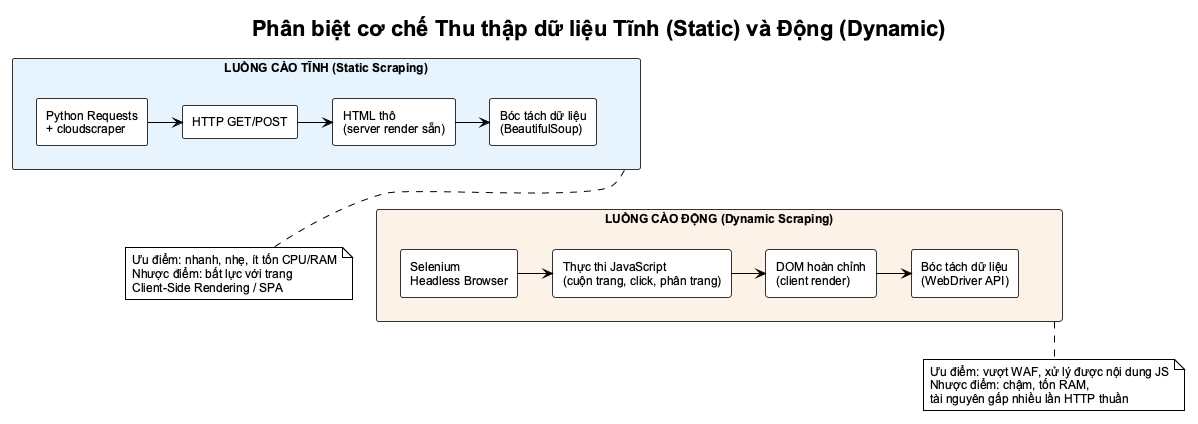
\includegraphics[width=0.85\textwidth]{image2_1}
    \caption{Phân biệt cơ chế hoạt động của kỹ thuật thu thập dữ liệu tĩnh (Static Scraping) và thu thập dữ liệu động (Dynamic Scraping).}
    \label{fig:static_vs_dynamic}
\end{figure}

Khi triển khai hệ thống thu thập thông tin tuyển dụng, việc lựa chọn phương pháp cào dữ liệu tĩnh dựa trên giao thức truyền tải siêu văn bản (HTTP Requests) hay cào dữ liệu động bằng trình duyệt không giao diện (Headless Browser) quyết định trực tiếp đến hiệu năng và độ ổn định của toàn hệ thống \cite{ref6}.

Phương pháp cào dữ liệu tĩnh sử dụng các thư viện như Python Requests để gửi các yêu cầu GET hoặc POST trực tiếp đến máy chủ của trang tuyển dụng nhằm tải về mã nguồn HTML thô \cite{ref4}. Phương pháp này sở hữu ưu điểm vượt trội về tốc độ phản hồi nhanh, tiêu thụ băng thông thấp và không yêu cầu năng lực tính toán lớn của CPU \cite{ref8}.

Tuy nhiên, HTTP Requests tĩnh hoàn toàn bất lực trước thế hệ ứng dụng web hiện đại sử dụng cơ chế kết xuất phía máy khách (Client-Side Rendering) thông qua JavaScript hoặc các ứng dụng đơn trang (Single Page Applications) \cite{ref7}. Đối với các trang tin tuyển dụng có cơ chế tải dữ liệu động thông qua các hành vi cuộn chuột hoặc chuyển trang bất tuần tự, hệ thống bắt buộc phải chuyển sang sử dụng Headless Browser như Selenium \cite{ref6}.

Selenium hoạt động bằng cách khởi tạo một trình duyệt thực thụ chạy ngầm không có giao diện hiển thị, thiết lập kết nối thông qua giao thức chuẩn hóa của tổ chức World Wide Web (W3C WebDriver) để thực thi toàn bộ các đoạn mã JavaScript trên trang, tự động hóa các thao tác click chuột, điền biểu mẫu, giải quyết phân trang và kết xuất ra cây phân cấp đối tượng tài liệu (Document Object Model --- DOM) hoàn chỉnh trước khi tiến hành bóc tách dữ liệu \cite{ref7}. Điểm hạn chế lớn nhất của Selenium là tiêu tốn bộ nhớ RAM lớn, tốc độ chậm và đòi hỏi tài nguyên hệ thống cao hơn gấp nhiều lần so với các yêu cầu HTTP truyền thống \cite{ref8}.

Bên cạnh vấn đề về mặt công nghệ kết xuất, các rào cản bảo mật từ các nền tảng tuyển dụng lớn như ITViec, VietnamWorks, CareerViet hay LinkedIn tạo ra thách thức không nhỏ cho quá trình thu thập thông tin tự động \cite{ref2}. Các nền tảng này thường thiết lập các hệ thống tường lửa ứng dụng Web (Web Application Firewall --- WAF) như Cloudflare nhằm phát hiện và ngăn chặn bot. Các cơ chế phòng thủ tiêu biểu bao gồm kiểm tra thử thách JavaScript (JS Challenges), hệ thống xác thực Turnstile, phân tích hành vi bất thường, giới hạn tần suất yêu cầu từ một địa chỉ IP (Rate Limiting) và phản hồi mã lỗi 403 Forbidden. Để giải quyết triệt để rào cản này, hệ thống tích hợp thư viện chuyên dụng cloudscraper \cite{ref13}.

Thư viện này hoạt động bằng cách tích hợp các công cụ thực thi JavaScript ngay trong tiến trình Python để giải quyết tự động các thuật toán thử thách của Cloudflare mà không cần khởi chạy một trình duyệt hoàn chỉnh \cite{ref13}. Đồng thời, cloudscraper thực hiện giả lập chữ ký mã hóa TLS (TLS Fingerprinting) kết hợp với việc thay đổi linh hoạt các tiêu đề HTTP (HTTP Headers) bao gồm chuỗi nhận diện trình duyệt (User-Agent) khớp với các thiết bị di động hoặc máy tính thực tế nhằm vượt qua cơ chế nhận diện bot của WAF \cite{ref16}.

\textbf{Đánh giá và lý giải lựa chọn:} Đối với bài toán cụ thể của hệ thống CareerNova, việc chỉ dùng một trong hai phương pháp đều không tối ưu: cào tĩnh nhanh nhưng bị chặn bởi WAF Cloudflare; cào động vượt WAF nhưng chậm và tốn tài nguyên nếu dùng cho toàn bộ hàng nghìn tin tuyển dụng. Yêu cầu nghiệp vụ về \textit{tính bền vững và hiệu năng} dẫn đến quyết định thiết kế một \textbf{cơ chế dự phòng hai tầng (Two-tier Fallback Mechanism)}: hệ thống ưu tiên cào tĩnh để đạt tốc độ tối đa; khi gặp tường lửa WAF chặn, hệ thống tự động kích hoạt luồng dự phòng chuyển sang Headless Browser với plugin chống phát hiện (Undetected ChromeDriver) và cơ chế xoay vòng proxy, đồng thời áp dụng giãn cách thời gian truy cập ngẫu nhiên để tiếp tục duy trì hoạt động thu thập dữ liệu \cite{dynamicwebscraping}.

Vì vậy, trong hệ thống đề xuất, sự kết hợp giữa cào tĩnh (qua Requests và cloudscraper) và cào động dự phòng (qua Selenium Headless Browser) được lựa chọn nhằm tối ưu hóa đồng thời tốc độ thu thập và tỷ lệ thành công đối với các nền tảng tuyển dụng có cơ chế chống bot nghiêm ngặt.

%==========================================================================

\subsection{Xác định yêu cầu xử lý và tổ chức dữ liệu thu thập}

Sau khi dữ liệu tuyển dụng được thu thập về, một thách thức nghiệp vụ tiếp theo được đặt ra: dữ liệu thô từ nhiều nguồn khác nhau (ITViec, VietnamWorks, LinkedIn...) có định dạng HTML và cấu trúc nội dung hoàn toàn không đồng nhất. Dữ liệu này cần được chuẩn hóa và tổ chức vào một cấu trúc nhất quán để phục vụ cho các module phân tích và trực quan hóa ở tầng trên. Yêu cầu nghiệp vụ cụ thể bao gồm:
\begin{itemize}
    \item Loại bỏ các thẻ HTML rác, ký tự đặc biệt, khoảng trắng thừa từ văn bản thô.
    \item Trích xuất các trường thông tin có cấu trúc (chức danh, kỹ năng, mức lương, địa điểm) từ mô tả công việc dạng tự do.
    \item Chuẩn hóa các biến thể tên gọi kỹ năng về một từ điển thống nhất (ví dụ: ``ReactJS'', ``React.js'', ``React'' đều cùng một thực thể).
    \item Lưu trữ kết quả vào cơ sở dữ liệu quan hệ để phục vụ truy vấn và trực quan hóa tức thời.
\end{itemize}

\subsection{Quy trình trích xuất, biến đổi và lưu trữ dữ liệu trong phân tích dữ liệu lớn}

Trong kiến trúc của các hệ thống thông tin hướng dữ liệu lớn, việc thiết lập một luồng xử lý dữ liệu chuẩn hóa đóng vai trò cốt lõi trong việc đảm bảo tính toàn vẹn và chất lượng của dữ liệu đầu ra \cite{ref8}. Hệ thống áp dụng phương pháp luận Trích xuất -- Biến đổi -- Nạp (Extract -- Transform -- Load --- ETL) được đề xuất bởi chuyên gia kho dữ liệu Ralph Kimball \cite{ref8}.

Theo Kimball, hệ thống ETL đóng vai trò như một phân xưởng chuẩn bị dữ liệu (Data Staging Area) \cite{ref15}. Đây là nơi tiếp nhận các nguồn dữ liệu thô, không đồng nhất, tiến hành làm sạch, loại bỏ các lỗi sai lệch, áp dụng các quy tắc nghiệp vụ để đồng nhất hóa ngữ nghĩa, trước khi tổ chức sắp xếp dữ liệu vào các cấu trúc bảng chuẩn hóa nhằm phục vụ cho các phân tích và hiển thị trực quan tiếp theo \cite{ref8}. Tiến trình này mặc dù hoạt động ngầm nhưng lại chiếm tới hơn 70\% nỗ lực và tài nguyên trong việc xây dựng một hệ thống thông tin hoàn chỉnh.

\begin{figure}[H]
    \centering
    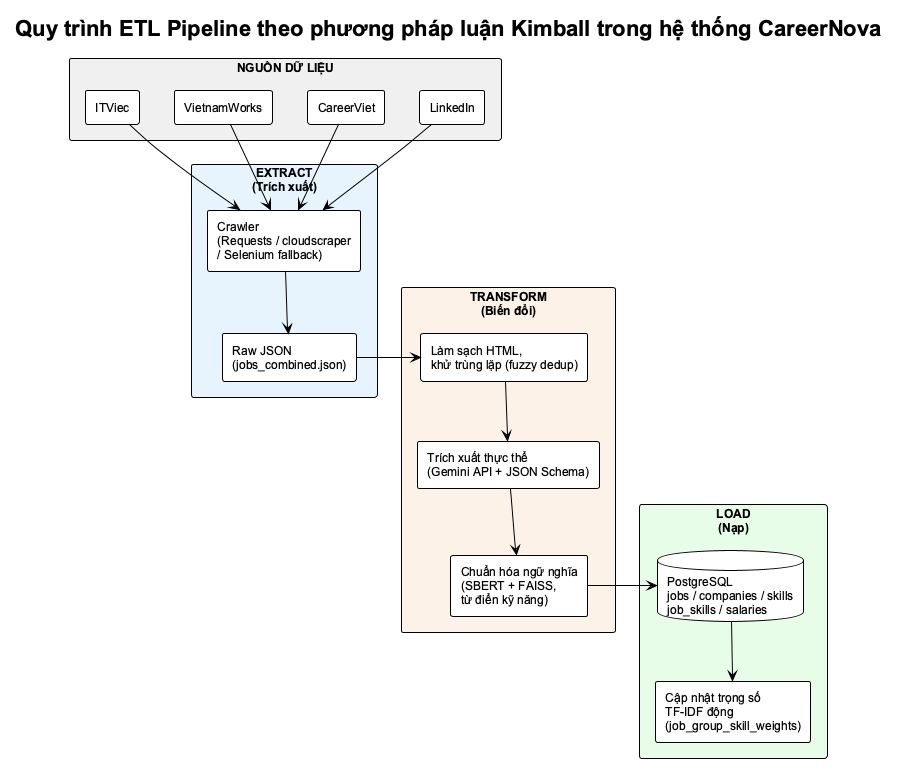
\includegraphics[width=0.90\textwidth]{image2_2}
    \caption{Quy trình tổng quát của tiến trình trích xuất, biến đổi và nạp dữ liệu (ETL Pipeline) theo phương pháp luận Kimball.}
    \label{fig:etl_pipeline}
\end{figure}


\textbf{Giai đoạn Trích xuất (Extract):} Hệ thống thực hiện thu thập dữ liệu phi cấu trúc từ các nguồn trang tuyển dụng khác nhau. Dữ liệu sau khi cào về được lưu trữ nguyên bản dưới dạng tệp tin JSON thô (raw JSON) tại phân vùng đệm của hệ thống \cite{ref22}. Việc lưu trữ dữ liệu thô giúp đảm bảo khả năng khôi phục hoặc tái xử lý dữ liệu từ đầu khi có sự thay đổi về quy tắc biến đổi mà không cần phải tiến hành cào lại từ trang web gốc, giảm thiểu việc tải nặng lên máy chủ đối tác và tuân thủ các quy tắc lịch sự trong thu thập dữ liệu \cite{ref24}.

\textbf{Giai đoạn Biến đổi (Transform):} Đây là giai đoạn quan trọng và phức tạp nhất của luồng xử lý \cite{ref22}. Đầu tiên, hệ thống thực hiện các bước tiền xử lý cơ bản bằng cách loại bỏ các thẻ định dạng HTML rác, các ký tự đặc biệt không mong muốn và chuẩn hóa khoảng trắng thông qua các biểu thức chính quy. Tiếp theo, do mô tả công việc (Job Description --- JD) mang tính phi cấu trúc cao, hệ thống gọi giao diện lập trình ứng dụng Gemini API để thực hiện trích xuất thực thể thông tin chuyên sâu bao gồm chức danh công việc, yêu cầu kỹ năng và các chế độ phúc lợi \cite{ref28}. Do các kỹ năng tuyển dụng thường được viết dưới dạng các thuật ngữ không đồng nhất, hệ thống tiếp tục thực hiện bước chuẩn hóa ngữ nghĩa (Semantic Normalization) \cite{ref24}. Các thực thể kỹ năng bóc tách được ánh xạ vào một từ điển kỹ năng chuẩn hóa duy nhất thông qua mô hình biểu diễn vector nhằm đảm bảo tính nhất quán ngữ nghĩa \cite{ref30}. Đây chính là quá trình thiết lập các chiều dữ liệu chuẩn hóa (Conformed Dimensions) theo lý thuyết Kimball, cho phép kết nối dữ liệu từ nhiều nguồn tuyển dụng khác nhau trên một hệ quy chiếu chung \cite{ref15}.

\textbf{Giai đoạn Nạp (Load):} Dữ liệu sau khi được làm sạch và chuẩn hóa ngữ nghĩa sẽ được chuyển đổi sang cấu trúc quan hệ để nạp vào hệ quản trị cơ sở dữ liệu PostgreSQL \cite{ref22}. Để tối ưu hóa hiệu năng truy vấn, tránh dư thừa dữ liệu và hỗ trợ trực quan hóa thời gian thực, cơ sở dữ liệu được tổ chức theo mô hình quan hệ chuẩn hóa cao bao gồm các bảng chính: bảng công việc (\texttt{jobs} lưu trữ các thông tin chung về vị trí tuyển dụng, công ty, mức lương, địa điểm), bảng kỹ năng (\texttt{skills} lưu trữ từ điển kỹ năng chuẩn hóa, đồng thời lưu giữ trường số liệu Document Frequency đại diện cho số lượng tin tuyển dụng chứa kỹ năng nhằm phục vụ tính toán trọng số IDF động) và bảng liên kết đa-đa (\texttt{job\_skills} lưu trữ liên kết giữa các công việc và các kỹ năng tương ứng kèm theo trọng số TF-IDF được tính toán thời gian thực từ tập dữ liệu thị trường) \cite{ref27}. Hơn nữa, kết quả tính toán chi tiết của bộ so khớp (Matching Engine) bao gồm cấu trúc biểu đồ Radar (\texttt{radar\_data}) và báo cáo khoảng cách kỹ năng (\texttt{gap\_report}) sẽ được đóng gói dưới định dạng JSONB để nạp trực tiếp vào cơ sở dữ liệu PostgreSQL. Thiết kế này giúp tối ưu hóa hiệu năng truy vấn thời gian thực ở tầng trực quan hóa mà không cần phải tính toán lại nhiều lần.

Vì vậy, trong hệ thống đề xuất, quy trình ETL theo mô hình Kimball được triển khai để biến dữ liệu tuyển dụng thô từ nhiều nguồn phi cấu trúc thành một kho dữ liệu PostgreSQL nhất quán, đồng thời tính toán động và lưu trữ trọng số TF-IDF cùng kết quả so khớp dạng JSONB để phục vụ trực quan hóa tức thời.

%==========================================================================

\subsection{Yêu cầu trực quan hóa thông tin hỗ trợ ra quyết định}

Sau khi dữ liệu tuyển dụng đã được chuẩn hóa và lưu trữ, yêu cầu nghiệp vụ tiếp theo là trình bày dữ liệu theo cách giúp sinh viên dễ dàng nhận diện khoảng cách năng lực và ra quyết định nghề nghiệp mà không cần kiến thức phân tích dữ liệu chuyên sâu. Yêu cầu này trực tiếp định hướng thiết kế các thành phần giao diện trực quan hóa.

\subsection{Nguyên lý trực quan hóa thông tin hỗ trợ ra quyết định}

\textbf{Trực quan hóa thông tin} (Information Visualization) là lĩnh vực nghiên cứu tập trung vào việc sử dụng các biểu diễn đồ họa tương tác để khai thác khả năng nhận thức thị giác, nhằm phát hiện các mẫu ẩn, xu hướng và mối quan hệ trong tập dữ liệu phức tạp \cite{card1999readings}. Card, Mackinlay và Shneiderman (1999) định nghĩa đây là ``việc sử dụng biểu diễn trực quan được máy tính hỗ trợ từ dữ liệu trừu tượng để khuếch đại nhận thức (amplify cognition)'' \cite{card1999readings}.

Nguyên lý định hướng thiết kế phổ biến nhất trong lĩnh vực này là \textbf{mantra trực quan hóa} của Shneiderman (1996): \textit{``Overview first, zoom and filter, then details on demand''} \cite{shneiderman1996eyes}. Theo nguyên lý này, giao diện cần dẫn dắt người dùng qua ba tầng tương tác: (i) nhìn thấy bức tranh tổng quan, (ii) thu hẹp dữ liệu theo các thuộc tính phù hợp và (iii) chỉ xem chi tiết khi đã xác định được vấn đề cần tìm hiểu. Cách tiếp cận này giảm tải nhận thức vì người dùng không phải đọc đồng thời toàn bộ dữ liệu thô và có thể đưa ra quyết định theo từng tầng thông tin.

Tufte (2001) nhấn mạnh rằng thiết kế đồ họa xuất sắc phải tối đa hóa tỷ số dữ liệu-mực vẽ (data-ink ratio) --- mọi yếu tố đồ họa đều phải mang thông tin có giá trị \cite{tufte2001visual}. Few (2006) mở rộng nguyên tắc này sang dashboard phân tích: dashboard cần ưu tiên thông tin quan trọng nhất trên một màn hình, sử dụng nhất quán các thuộc tính tiền chú ý (pre-attentive attributes) như vị trí, độ dài, màu sắc tương phản và kích thước tương đối để người dùng nhận diện xu hướng hoặc ngoại lệ nhanh chóng \cite{few2006dashboard}. Vì vậy, màu sắc trong CareerNova được dùng có ngữ nghĩa cố định: xanh lá cho mức đáp ứng tốt, vàng cho mức cần cải thiện và đỏ cho thiếu hụt; không dùng màu sắc chỉ để trang trí.

\textbf{Ứng dụng vào hệ thống CareerNova:} Dựa trên các nguyên lý trên và giao diện hiện tại của hệ thống, các thành phần trực quan hóa được lựa chọn theo câu hỏi ra quyết định cụ thể của sinh viên:

\begin{enumerate}
    \item \textbf{Thẻ chỉ số tổng quan:} Hiển thị số tin đang mở, số công ty đang tuyển và số cơ hội thực tập theo bộ lọc. Đây là lớp ``overview first'', giúp người dùng nắm quy mô thị trường trước khi xem biểu đồ chi tiết.

    \item \textbf{Biểu đồ vùng (AreaChart):} Thể hiện xu hướng số tin tuyển dụng theo thời gian, đồng thời so sánh tổng số tin với số vị trí làm việc từ xa. Người dùng quan sát được biến động nhu cầu tuyển dụng và xác định giai đoạn nên ưu tiên tìm việc.

    \item \textbf{Bản đồ cây (Treemap):} Biểu diễn tỷ trọng các nhóm kỹ năng hoặc lĩnh vực trong thị trường. Diện tích mỗi ô tỷ lệ với số tin tuyển dụng; do đó người dùng nhanh chóng nhận biết nhóm có nhu cầu nổi trội mà không cần đọc bảng dữ liệu dài.

    \item \textbf{Biểu đồ cột xếp hạng và danh sách kỹ năng tăng trưởng:} Danh sách ``Top 10 kỹ năng được yêu cầu'' dùng độ dài thanh để so sánh số tin theo kỹ năng; danh sách ``Kỹ năng tăng trưởng nhanh'' nhấn mạnh tốc độ thay đổi bằng màu cam và phần trăm tăng trưởng. Hai thành phần giúp chuyển từ quan sát tổng quan sang quyết định kỹ năng cần ưu tiên học.

    \item \textbf{Biểu đồ Radar và Gap Report:} RadarChart biểu diễn đồng thời năng lực hiện tại của người dùng và ngưỡng yêu cầu thị trường trên hệ trục đa chiều. Báo cáo khoảng cách kỹ năng bổ sung danh sách đạt yêu cầu, đạt một phần và còn thiếu, giúp người dùng hiểu nguyên nhân phía sau điểm phù hợp và lựa chọn kỹ năng cần cải thiện.
\end{enumerate}

Tất cả thành phần thị trường đều dùng chung bộ lọc theo khu vực, khoảng thời gian và loại hình công việc. Cách tổ chức này hiện thực hóa đầy đủ mantra của Shneiderman: người dùng xem tổng quan qua thẻ chỉ số và xu hướng, thu hẹp phạm vi bằng bộ lọc, sau đó xem chi tiết qua danh sách vị trí, kỹ năng hoặc báo cáo khoảng cách. Màu sắc được dùng có ngữ nghĩa cố định: xanh lá cho trạng thái đáp ứng tốt, vàng cho mức cần cải thiện, đỏ cho kỹ năng thiếu và cam cho xu hướng tăng nhanh; vì vậy màu sắc hỗ trợ nhận biết thay vì chỉ mang tính trang trí. Luồng dữ liệu từ cơ sở dữ liệu đến các thành phần trực quan hóa được mô tả trong Hình~\ref{fig:visualization_theory}.

\begin{figure}[H]
    \centering
    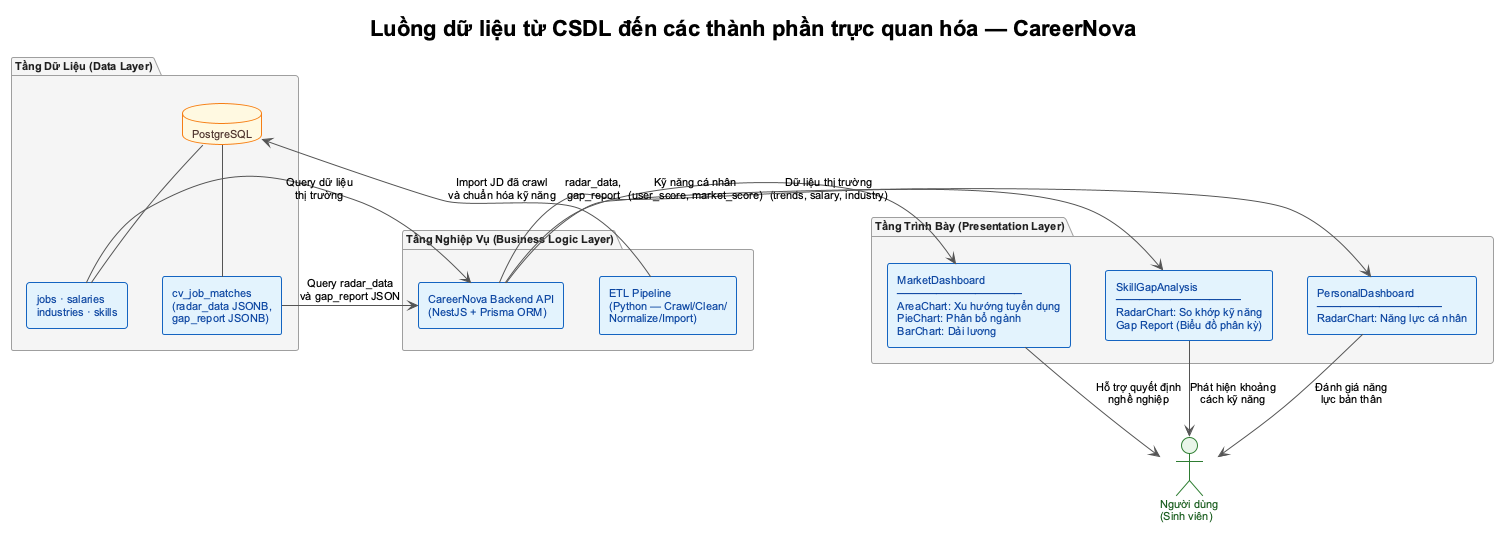
\includegraphics[width=0.9\textwidth]{visualization_theory}
    \caption{Luồng dữ liệu từ cơ sở dữ liệu đến các thành phần trực quan hóa trong hệ thống CareerNova.}
    \label{fig:visualization_theory}
\end{figure}

Tóm lại, việc lựa chọn biểu đồ trong CareerNova dựa trên câu hỏi ra quyết định thay vì dựa trên tính trang trí: biểu đồ xu hướng trả lời câu hỏi về thời điểm, Treemap trả lời câu hỏi về nhóm nhu cầu nổi trội, biểu đồ xếp hạng và danh sách tăng trưởng trả lời câu hỏi nên ưu tiên kỹ năng nào, còn Radar Chart và Gap Report trả lời câu hỏi về năng lực cần bổ sung. Nhờ tuân thủ các nguyên lý của Card, Shneiderman, Tufte và Few, người dùng không cần kiến thức phân tích dữ liệu chuyên sâu vẫn có thể nhận diện khoảng cách năng lực, theo dõi xu hướng thị trường và điều chỉnh định hướng nghề nghiệp qua các biểu đồ tương tác.

%==========================================================================

\section{Giải pháp so khớp hồ sơ}

\subsection{Xác định yêu cầu nghiệp vụ của bài toán so khớp hồ sơ}

Một yêu cầu nghiệp vụ trung tâm của hệ thống CareerNova là đánh giá \textit{mức độ phù hợp} giữa năng lực của sinh viên (thể hiện qua CV) và yêu cầu các vị trí tuyển dụng (thể hiện qua JD) theo cách có ý nghĩa hơn so với việc đơn thuần đếm từ khóa trùng khớp. Phân tích yêu cầu này làm nổi lên hai vấn đề cốt lõi cần giải quyết ở tầng thuật toán:

\begin{itemize}
    \item \textbf{Vấn đề 1 --- Đo lường tương đồng ngữ nghĩa:} Cần một phương pháp biểu diễn và so sánh ý nghĩa của các kỹ năng ngay cả khi chúng được diễn đạt khác nhau về từ ngữ (``JS'' vs ``JavaScript'', ``lãnh đạo nhóm'' vs ``team leadership'').
    \item \textbf{Vấn đề 2 --- Phân biệt tầm quan trọng của kỹ năng:} Không phải mọi kỹ năng đều quan trọng như nhau. Kỹ năng hiếm và chuyên sâu (PyTorch, Kubernetes) cần được trọng số hóa cao hơn kỹ năng phổ biến (Git, HTML) để điểm so khớp phản ánh đúng thực tế thị trường.
\end{itemize}

Hai vấn đề này định hướng việc lựa chọn các kỹ thuật biểu diễn và so sánh vector ngữ nghĩa được phân tích ở các mục tiếp theo.

\subsection{Lý thuyết không gian vector và kỹ thuật tạo vector nhúng}

Mô hình Không gian Vector (Vector Space Model --- VSM) là một nền tảng lý thuyết kinh điển trong xử lý ngôn ngữ tự nhiên (Natural Language Processing --- NLP) và tìm kiếm thông tin, biểu diễn tài liệu văn bản dưới dạng các điểm hoặc vector trong một không gian số học đa chiều \cite{ref21}. Trong không gian này, khoảng cách hình học giữa các vector tỷ lệ thuận với mức độ tương đồng về mặt nội dung giữa các tài liệu tương ứng \cite{ref38}. Sự phát triển của các kỹ thuật biểu diễn từ ngữ đã chuyển dịch từ các vector thưa tần suất (như TF-IDF --- vốn bỏ qua ngữ cảnh và quan hệ đồng nghĩa) sang các vector nhúng dày đặc (Dense Embeddings), nơi các giá trị số học biểu diễn các đặc trưng ngữ nghĩa ẩn của từ ngữ trong một không gian liên tục \cite{ref30}.

Để giải quyết bài toán biểu diễn ngữ nghĩa ở cấp độ câu và cụm từ phức tạp trong tin tuyển dụng và hồ sơ ứng viên, Nils Reimers và Iryna Gurevych đã đề xuất mô hình Sentence-BERT (SBERT) vào năm 2019 \cite{ref38}. SBERT cải tiến mô hình tiền huấn luyện BERT bằng cách sử dụng cấu trúc mạng song sinh (Siamese Network) và mạng sinh ba (Triplet Network) để tối ưu hóa trọng số của mô hình \cite{ref12}. Kiến trúc mạng song sinh của SBERT bao gồm hai nhánh BERT song song có chia sẻ hoàn toàn bộ tham số trọng số \cite{ref38}. Khi xử lý cặp văn bản đầu vào $(s_1, s_2)$, mỗi câu sẽ được đưa qua một nhánh mạng độc lập để trích xuất các trạng thái ẩn cuối cùng:
\begin{equation}
    H_i = \text{BERT}(s_i), \quad i \in \{1, 2\}
\end{equation}

Sau đó, một phép toán lấy trung bình trọng số (Mean Pooling) được áp dụng trên toàn bộ các vector biểu diễn token của câu ở lớp đầu ra để chuyển đổi ma trận trạng thái ẩn có kích thước biến thiên thành một vector nhúng có kích thước cố định $\mathbf{u}$ biểu diễn trọn vẹn ngữ nghĩa của toàn bộ câu \cite{ref20}. SBERT được huấn luyện thông qua các mục tiêu tối ưu như hàm mất mát phân loại (Classification Loss) dựa trên việc liên kết các vector hoặc hàm mất mát hồi quy (Regression Loss) so khớp trực tiếp với điểm tương đồng mục tiêu \cite{ref42}. Phát minh mang tính đột phá của SBERT nằm ở chỗ nó cho phép mã hóa độc lập từng câu thành vector nhúng cố định \cite{ref21}. Điều này cho phép hệ thống tính toán trước (precompute) và lập chỉ mục các vector biểu diễn năng lực của hàng triệu ứng viên hoặc công việc một lần duy nhất \cite{ref30}. Khi cần so khớp, hệ thống chỉ việc thực hiện các phép so sánh vector đơn giản (như tính Cosine) trong thời gian vài phần nghìn giây, giải quyết triệt để nút thắt cổ chai về mặt hiệu năng của kiến trúc BERT Cross-Encoder truyền thống \cite{ref12}.

Trong bối cảnh xây dựng công cụ so khớp hồ sơ cục bộ (local engine) hoạt động tối ưu trên máy chủ có giới hạn về tài nguyên phần cứng, mô hình \texttt{all-MiniLM-L6-v2} thuộc thư viện Sentence Transformers được lựa chọn làm giải pháp biểu diễn vector cốt lõi \cite{ref26}. Được phát triển dựa trên phương pháp chắt lọc tri thức (Knowledge Distillation) từ kiến trúc MiniLM của Microsoft, mô hình này sở hữu cấu hình kỹ thuật cực kỳ tinh gọn \cite{ref26}:

\begin{figure}[H]
    \centering
    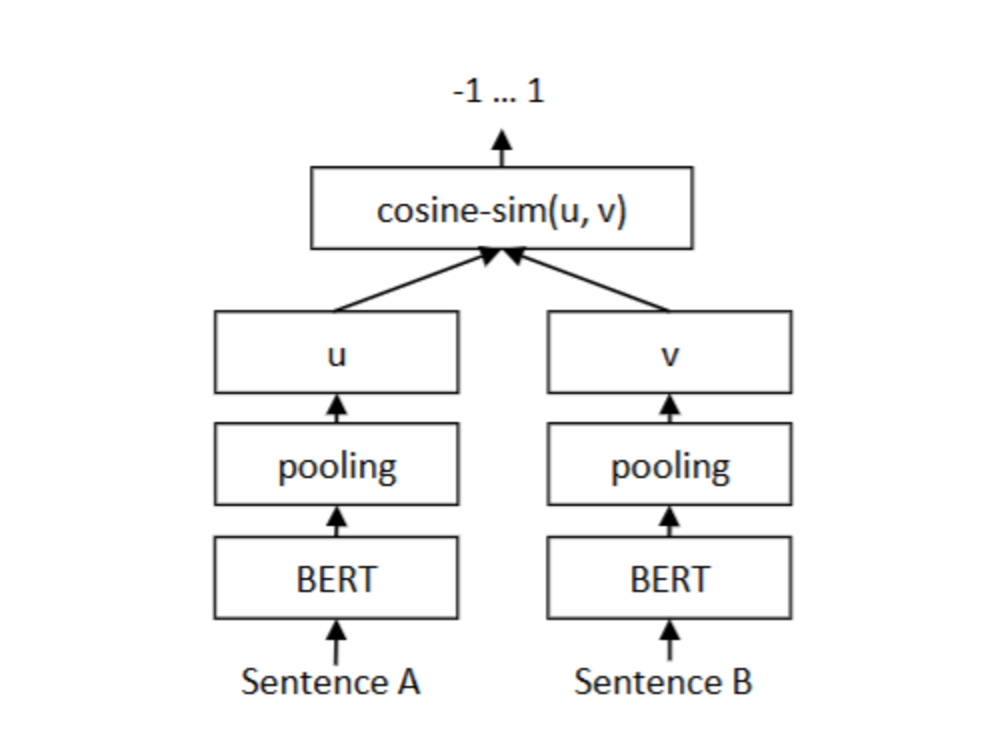
\includegraphics[width=0.75\textwidth]{image2_3}
    \caption{Kiến trúc SBERT được sử dụng trong suy luận để tính điểm tương đồng ngữ nghĩa.}
    \label{fig:sbert_arch}
\end{figure}

\begin{itemize}
    \item \textbf{Số lượng tầng biến đổi (Layers):} 6 tầng Transformer (so với 12 tầng của BERT-base) \cite{ref45}.
    \item \textbf{Kích thước tham số (Parameter Count):} Khoảng 22 triệu tham số (chỉ bằng 1/5 kích thước của BERT-base) \cite{ref45}.
    \item \textbf{Chiều của vector nhúng (Embedding Size):} 384 chiều liên tục \cite{ref26}.
    \item \textbf{Độ dài chuỗi đầu vào tối đa (Max Sequence Length):} 256 tokens \cite{ref26}.
    \item \textbf{Dung lượng đĩa cứng (Model Size):} Khoảng 80 MB \cite{ref48}.
\end{itemize}

Lý do lựa chọn \texttt{all-MiniLM-L6-v2} xuất phát từ sự cân bằng hoàn hảo giữa hiệu năng tính toán và chất lượng biểu diễn ngữ nghĩa \cite{ref30}. Mô hình được huấn luyện tự giám sát trên tập dữ liệu khổng lồ chứa hơn 1 tỷ cặp câu chất lượng cao, bao gồm cả tập dữ liệu tìm kiếm ngữ nghĩa MS MARCO \cite{ref26}. Nhờ đó, dù có dung lượng bộ nhớ cache siêu nhẹ (80 MB) và tốc độ mã hóa cực nhanh (vận hành trên CPU thông thường đạt hiệu năng vượt trội, lên tới hơn 14.200 câu/giây trên GPU) \cite{ref45}, mô hình vẫn duy trì khả năng biểu diễn ngữ nghĩa vượt trội, tương đương hoặc thậm chí vượt qua các mô hình lớn hơn nhiều trong các tác vụ tìm kiếm ngữ nghĩa và so khớp văn bản ngắn \cite{ref45}. Vì vậy, trong hệ thống đề xuất, mô hình nhúng cục bộ \texttt{all-MiniLM-L6-v2} được lựa chọn để thực hiện mã hóa các thực thể kỹ năng một cách nhanh chóng và chính xác trực tiếp trên máy chủ cục bộ mà không tốn chi phí gọi API bên thứ ba.

%==========================================================================

\subsection{Phương pháp định lượng hóa độ tương đồng ngữ nghĩa bằng độ đo Cosine và Trọng số TF-IDF từ thị trường}

Để lượng hóa mức độ tương đồng về mặt năng lực giữa hồ sơ ứng viên (CV) và mô tả yêu cầu công việc (JD), hệ thống áp dụng độ đo Cosine (Cosine Similarity) \cite{ref42}. Về mặt toán học, độ đo Cosine giữa hai vector đa chiều phi không $\mathbf{u}$ và $\mathbf{v}$ được định nghĩa là tỷ số giữa tích vô hướng của hai vector và tích độ dài (chuẩn L2) của chúng:
\begin{equation}
    \text{cosine}(\mathbf{u}, \mathbf{v}) = \frac{\mathbf{u} \cdot \mathbf{v}}{\|\mathbf{u}\|_2 \cdot \|\mathbf{v}\|_2} = \frac{\sum_{k=1}^{d} u_k v_k}{\sqrt{\sum_{k=1}^{d} u_k^2} \cdot \sqrt{\sum_{k=1}^{d} v_k^2}}
\end{equation}
Trong đó $d = 384$ là số chiều của không gian vector biểu diễn bởi mô hình \texttt{all-MiniLM-L6-v2} \cite{ref26}. Giá trị của độ đo Cosine nằm trong khoảng $[-1, 1]$, thể hiện mức độ trùng khớp ngữ nghĩa từ hoàn toàn khác biệt đến hoàn toàn tương đồng.

Để tối ưu hóa hiệu năng tính toán khi so khớp hàng loạt hồ sơ trực tuyến, giả sử các vector nhúng đầu ra đã được chuẩn hóa đơn vị (Unit Vectors):
\begin{equation}
    \|\hat{\mathbf{u}}\|_2 = \|\hat{\mathbf{v}}\|_2 = 1
\end{equation}
Khi đó, công thức tính độ tương đồng Cosine được rút gọn về tích vô hướng (Dot Product):
\begin{equation}
    \text{cosine}(\hat{\mathbf{u}}, \hat{\mathbf{v}}) = \hat{\mathbf{u}} \cdot \hat{\mathbf{v}} = \sum_{k=1}^{d} \hat{u}_k \hat{v}_k
\end{equation}
Điều này loại bỏ các phép toán tính căn bậc hai và phép chia trong vòng lặp so khớp quy mô lớn, giúp giảm thiểu đáng kể số chu kỳ lệnh của CPU/GPU và cho phép thực hiện hàng triệu phép so khớp trong thời gian thực \cite{airesumematching}.

Chứng minh trên chỉ ra rằng, đối với các vector đã chuẩn hóa đơn vị, việc tính độ tương đồng Cosine thực chất tương đương với việc thực hiện phép nhân Tích vô hướng (Dot Product). Việc loại bỏ hoàn toàn các phép toán phức tạp như tính căn bậc hai và phép chia trong vòng lặp so khớp quy mô lớn giúp giảm thiểu đáng kể số lượng chu kỳ lệnh của CPU/GPU, cho phép hệ thống thực hiện hàng triệu phép so khớp trong thời gian thực với độ trễ tối thiểu \cite{ref21}.

Tuy nhiên, trong bài toán so khớp hồ sơ nhân sự thực tế, không phải tất cả các kỹ năng được yêu cầu trong mô tả công việc (JD) đều có vai trò đóng góp như nhau vào tổng điểm đánh giá của ứng viên. Nếu sử dụng độ đo tương đồng không trọng số, các kỹ năng cực kỳ phổ biến và dễ đạt được (ví dụ: Git, SQL, Microsoft Office, HTML/CSS) sẽ vô tình làm lu mờ sự thiếu hụt hoặc mức độ tương đồng thấp ở các kỹ năng cốt lõi, mang tính chất quyết định của công việc (ví dụ: PyTorch, CI/CD, Kubernetes). Để giải quyết triệt để vấn đề này, đề tài xây dựng giải pháp định lượng hóa trọng số kỹ năng động dựa trên công thức TF-IDF (Term Frequency -- Inverse Document Frequency) được tính toán trực tiếp từ kho ngữ liệu tin tuyển dụng thực tế cào từ thị trường Việt Nam \cite{ref52}.

Mô hình toán học của cơ chế tính trọng số này được thiết lập như sau. Gọi $\mathcal{D} = \{d_1, d_2, \ldots, d_N\}$ là tập hợp (corpus) chứa tất cả $N$ tin tuyển dụng đã thu thập và lưu trữ thành công trong PostgreSQL. Với một tin tuyển dụng (JD) cụ thể $d_j$, gọi $S_j$ là tập hợp các kỹ năng yêu cầu được trích xuất từ JD đó.

\textbf{Tần suất Kỹ năng (Term Frequency --- $\text{TF}$)} thể hiện mức độ nổi bật của kỹ năng $s_i$ trong JD $d_j$. Do kỹ năng thường xuất hiện dưới dạng thực thể đơn lẻ (presence/absence) trong danh sách yêu cầu của JD, tần suất $\text{TF}$ được định nghĩa theo dạng chuẩn hóa nhị phân \cite{ref55}:
\begin{equation}
    \text{TF}(s_i, d_j) = \begin{cases} 1 & \text{nếu } s_i \in S_j \\ 0 & \text{ngược lại} \end{cases}
\end{equation}

\textbf{Nghịch đảo Tần suất Văn bản (Inverse Document Frequency --- $\text{IDF}$)} đo lường mức độ đặc trưng và tính khan hiếm của kỹ năng $s_i$ trên toàn bộ thị trường lao động Việt Nam \cite{ref56}:
\begin{equation}
    \text{IDF}(s_i, \mathcal{D}) = \log\left(\frac{N}{|\{d \in \mathcal{D} : s_i \in S_d\}|}\right)
\end{equation}
Trong đó $N$ là tổng số tin tuyển dụng, và $|\{d \in \mathcal{D} : s_i \in S_d\}|$ là số tin tuyển dụng chứa kỹ năng $s_i$.

\textbf{Trọng số TF-IDF kết hợp} của kỹ năng $s_i$ thuộc JD $d_j$ được xác định bằng tích của hai thành phần \cite{ref56}:
\begin{equation}
    w(s_i, d_j) = \text{TF}(s_i, d_j) \times \text{IDF}(s_i, \mathcal{D})
\end{equation}

Nhờ mô hình này, kỹ năng xuất hiện tràn lan (IDF $\approx 0$) sẽ có trọng số tiến về 0, giảm ảnh hưởng của kỹ năng phổ biến. Ngược lại, kỹ năng chuyên sâu và hiếm có IDF lớn, đẩy trọng số lên cao để tạo lực đẩy quyết định cho điểm số.

Cuối cùng, tổng điểm tương thích \textbf{Match Score} giữa hồ sơ CV của ứng viên và yêu cầu JD của công việc được xác định bằng công thức trung bình có trọng số TF-IDF của các độ tương đồng kỹ năng \cite{ref52}:
\begin{equation}
    \text{MatchScore}(\text{CV}, d_j) = \frac{\sum_{s_i \in S_j} w(s_i, d_j) \cdot \text{cosine}(\mathbf{e}_{s_i}^{\text{CV}}, \mathbf{e}_{s_i}^{\text{JD}})}{\sum_{s_i \in S_j} w(s_i, d_j)}
\end{equation}

Áp dụng rút gọn tích vô hướng cho các vector đã chuẩn hóa đơn vị ($\|\hat{\mathbf{e}}\|_2 = 1$), công thức Match Score cuối cùng của hệ thống:
\begin{equation}
    \text{MatchScore}(\text{CV}, d_j) = \frac{\sum_{s_i \in S_j} w(s_i, d_j) \cdot \left(\hat{\mathbf{e}}_{s_i}^{\text{CV}} \cdot \hat{\mathbf{e}}_{s_i}^{\text{JD}}\right)}{\sum_{s_i \in S_j} w(s_i, d_j)}
\end{equation}

Vì vậy, trong hệ thống đề xuất, phương pháp tích vô hướng trên vector chuẩn hóa kết hợp trọng số TF-IDF từ thị trường thực tế được triển khai để tính Match Score chuẩn xác, tối ưu hóa hiệu năng thời gian thực và phản ánh chính xác xu thế cung -- cầu của thị trường lao động CNTT Việt Nam.

%==========================================================================

\subsection{Khảo sát các công cụ và thuật toán so khớp hồ sơ hiện có}

Quá trình tiến hóa công nghệ của các Hệ thống quản lý ứng viên (Applicant Tracking System --- ATS) trải qua bốn thế hệ phát triển rõ rệt, từ các bộ lọc từ khóa sơ khai cho đến các hệ thống trí tuệ nhân tạo hiện đại \cite{ref27}. Sự khác biệt giữa các thế hệ được thể hiện chi tiết trong Bảng~\ref{tab:ats_generations}.

\begin{longtable}{|L{2.2cm}|L{3cm}|L{3cm}|L{2.8cm}|L{1.5cm}|L{2cm}|}
\caption{So sánh các thế hệ hệ thống ATS theo công nghệ cốt lõi, ưu nhược điểm và chi phí vận hành.}
\label{tab:ats_generations} \\
\hline
\textbf{Thế hệ ATS} & \textbf{Công nghệ cốt lõi} & \textbf{Ưu điểm} & \textbf{Nhược điểm} & \textbf{Chi phí} & \textbf{Độ trễ (Latency)} \\
\hline
\endfirsthead
\hline
\textbf{Thế hệ ATS} & \textbf{Công nghệ cốt lõi} & \textbf{Ưu điểm} & \textbf{Nhược điểm} & \textbf{Chi phí} & \textbf{Độ trễ (Latency)} \\
\hline
\endhead
Thế hệ I: Rule-based &
Biểu thức chính quy (Regex), So khớp từ khóa chính xác (Keyword Matching) \cite{ref58}. &
Đơn giản, dễ triển khai, tốc độ xử lý tức thời, không tốn tài nguyên. &
Thất bại với từ đồng nghĩa, viết tắt \cite{ref40}. Dễ bị gian lận bằng nhồi từ khóa. &
Rất thấp &
Cực thấp ($<$10ms) \\
\hline
Thế hệ II: Machine Learning truyền thống &
Mô hình túi từ (Bag of Words), TF-IDF tĩnh, Naive Bayes, SVM, Word2Vec \cite{ref2}. &
Nhận diện tầm quan trọng từ dựa trên tần suất \cite{ref50}, bắt đầu hiểu quan hệ đồng nghĩa cơ bản. &
Không hiểu ngữ cảnh câu văn \cite{ref30}, đòi hỏi dữ liệu gán nhãn lớn. &
Thấp &
Thấp (10--50ms) \\
\hline
Thế hệ III: Deep Learning (Bi-Encoder) &
Sentence-BERT (SBERT), Siamese Networks, không gian vector nhúng \cite{ref21}. &
Biểu diễn ngữ nghĩa câu xuất sắc \cite{ref45}. Cho phép tính trước vector nhúng để so khớp quy mô lớn. &
Đòi hỏi tài nguyên phần cứng mạnh (GPU) \cite{ref21}. Khó với tài liệu bố cục phức tạp \cite{ref36}. &
Trung bình &
Trung bình (50--200ms) \\
\hline
Thế hệ IV: LLM APIs &
Các mô hình ngôn ngữ lớn thương mại (GPT-4, Gemini, LLaMA), tác nhân AI (AI Agents) \cite{ref27}. &
Hiểu ngữ cảnh, bố cục và ngôn ngữ tự nhiên vô song \cite{ref36}. Khả năng tóm tắt và suy luận sâu sắc. &
Chi phí API tích lũy cực kỳ tốn kém khi xử lý dữ liệu lớn. Độ trễ phản hồi cao. &
Rất cao (tính phí theo Token) &
Rất cao (1--5 giây/yêu cầu) \\
\hline
\end{longtable}

Mặc dù các mô hình ngôn ngữ lớn thuộc Thế hệ IV thể hiện khả năng hiểu văn bản vượt trội, việc gửi trực tiếp toàn bộ nội dung của hàng nghìn hồ sơ ứng viên và tin tuyển dụng lên các API thương mại cho mỗi lần chạy so khớp là một giải pháp không khả thi đối với các dự án thực tế xét trên cả hai phương diện kinh tế và kỹ thuật \cite{ref36}. Về mặt kinh tế, chi phí sử dụng API sẽ tăng trưởng theo cấp số nhân khi số lượng hồ sơ cần đánh giá lớn. Về mặt kỹ thuật, độ trễ phản hồi của LLM API lên tới vài giây sẽ làm tê liệt khả năng hiển thị thời gian thực của các công cụ trực quan hóa thông tin tuyển dụng. Ngược lại, nếu chỉ dựa vào các mô hình nhúng cục bộ thuộc Thế hệ III để so khớp trực tiếp toàn bộ văn bản của CV và JD, hệ thống sẽ gặp phải sai số rất lớn do cấu trúc CV thường chứa nhiều thông tin nhiễu khiến vector nhúng của toàn bộ văn bản bị lệch hướng ngữ nghĩa \cite{ref27}.

Để giải quyết mâu thuẫn này, đề tài đề xuất một \textbf{giải pháp lai đột phá (Hybrid Approach)}, tách rời quy trình thành hai bước độc lập:

\begin{enumerate}
    \item \textbf{Bước bóc tách cấu trúc ngoại tuyến (Offline Structuring):} Sử dụng Gemini API (Thế hệ IV) để xử lý một lần duy nhất khi CV được tải lên hoặc khi tin tuyển dụng được cào về \cite{ref27}. Sức mạnh suy luận của LLM được khai thác triệt để để bóc tách chính xác các thực thể kỹ năng, chức danh công việc từ văn bản phi cấu trúc phức tạp thành dữ liệu bán cấu trúc JSON \cite{ref40}.
    \item \textbf{Bước so khớp trực tuyến (Online Matching Engine):} Khi người dùng thực hiện thao tác so khớp hoặc xem trực quan hóa, hệ thống sử dụng mô hình Sentence-BERT cục bộ \texttt{all-MiniLM-L6-v2} (Thế hệ III) kết hợp độ đo Cosine chuẩn hóa tích vô hướng và trọng số TF-IDF được tính động trực tuyến từ tập dữ liệu thị trường để tính toán Match Score trực tiếp trên các kỹ năng đã được cấu trúc hóa \cite{ref26}.
\end{enumerate}

Lập luận khoa học của giải pháp lai này dựa trên việc đặt đúng công nghệ vào đúng tác vụ: tận dụng khả năng hiểu bố cục xuất sắc của LLM để dọn dẹp và cấu trúc hóa dữ liệu, đồng thời tận dụng tốc độ tính toán vector vượt trội, chi phí bằng không và tính bảo mật của mô hình SBERT cục bộ kết hợp với trọng số TF-IDF có ý nghĩa phân loại cao cho khâu tìm kiếm và so khớp thời gian thực \cite{ref21}. Vì vậy, trong hệ thống đề xuất, giải pháp kiến trúc lai (Hybrid) kết hợp LLM API ngoại tuyến và SBERT trực tuyến có trọng số TF-IDF được lựa chọn để tối ưu hóa bài toán so khớp hồ sơ đạt hiệu năng cao và tiết kiệm chi phí vận hành.

%==========================================================================

\section{Trích xuất thực thể trong quản lý thị trường việc làm}

\subsection{Bài toán bóc tách thông tin kỹ năng, vị trí công việc từ văn bản}

Nhận diện thực thể tên (Named Entity Recognition --- NER) là một trong những tác vụ nền tảng nhất của xử lý ngôn ngữ tự nhiên, hướng tới việc tự động xác định các phân đoạn văn bản thô đại diện cho các thực thể cụ thể và phân loại chúng vào các nhóm ngữ nghĩa được định nghĩa trước \cite{ref30}. Khi được áp dụng vào lĩnh vực quản lý nhân sự (HR Domain), bài toán NER trở nên đặc thù và phức tạp hơn rất nhiều, đòi hỏi hệ thống phải bóc tách chính xác các thực thể cốt lõi bao gồm: chức danh công việc (Job Title), kỹ năng chuyên môn (Skills), trình độ học vấn, các chứng chỉ chuyên ngành và chế độ phúc lợi \cite{ref27}. Việc cấu trúc hóa thành công các thực thể này từ văn bản tự do là điều kiện tiên quyết để xây dựng các thuật toán so khớp chính xác và lập biểu đồ phân tích thị trường lao động hiệu quả.

Thách thức lớn nhất khi giải quyết tác vụ NER trong lĩnh vực nhân sự xuất phát từ tính phi cấu trúc cực kỳ cao của hồ sơ ứng viên (CV) \cite{ref36}. Ứng viên thường tự do trình bày hồ sơ cá nhân theo nhiều phong cách thẩm mỹ khác nhau, sử dụng các phần mềm thiết kế đa dạng dẫn đến định dạng tệp tin không đồng nhất (như PDF, DOCX, hoặc tệp ảnh quét) \cite{ref27}. Đối với các CV được lưu trữ dưới dạng ảnh quét hoặc PDF dạng ảnh, hệ thống bắt buộc phải tích hợp một lớp nhận diện ký tự quang học (Optical Character Recognition --- OCR) để khôi phục văn bản thô. Tuy nhiên, CV hiện đại thường áp dụng bố cục trình bày nhiều cột (multi-column layouts) hoặc dạng bảng lồng nhau nhằm tối ưu hóa diện tích hiển thị \cite{ref36}. Các công cụ đọc văn bản thông thường nếu chỉ quét tuần tự từ trái sang phải, từ trên xuống dưới sẽ làm đứt gãy hoàn toàn cấu trúc ngữ pháp của câu văn, trộn lẫn nội dung của hai cột khác biệt, dẫn đến việc phá hủy ngữ cảnh và khiến các mô hình NER truyền thống mất khả năng nhận diện thực thể chính xác.

Đặc biệt, đối với thị trường lao động ngành Công nghệ thông tin tại Việt Nam, bài toán trích xuất thực thể phải đối mặt với rào cản ngôn ngữ song ngữ Anh -- Việt rất phức tạp. Cả nhà tuyển dụng và ứng viên thường có thói quen viết xen lẫn hai ngôn ngữ ngay trong cùng một câu văn. Thêm vào đó, danh mục kỹ năng ngành IT vô cùng đa dạng, chứa nhiều thuật ngữ viết tắt, viết liền hoặc có nhiều biến thể ký tự khác nhau. Các mô hình NER truyền thống dựa trên các thuật toán học máy giám sát thường bộc lộ sự yếu kém do tập dữ liệu huấn luyện hạn chế, không thể bao phủ toàn bộ các biến thể ngôn ngữ lai này, dẫn đến tỷ lệ bỏ sót thực thể kỹ năng mới hoặc nhận diện sai lệch chức danh công việc ở mức cao \cite{ref27}. Vì vậy, trong hệ thống đề xuất, giải pháp nhận diện thực thể tên kết hợp OCR được triển khai để xử lý các CV song ngữ và đa dạng về cấu trúc trình bày một cách chuẩn xác, đảm bảo không bỏ sót thông tin năng lực của ứng viên.

%==========================================================================

\subsection{Ứng dụng mô hình ngôn ngữ lớn (LLM) và câu lệnh để chuẩn hóa dữ liệu}

Sự trỗi dậy của các mô hình ngôn ngữ lớn (Large Language Models --- LLMs) dựa trên kiến trúc Transformer tự chú ý đã mang lại một bước nhảy vọt về chất cho tác vụ bóc tách thông tin \cite{ref27}. Nhờ được huấn luyện trên các kho ngữ liệu khổng lồ đa ngôn ngữ, các LLM hiện đại như Google Gemini sở hữu khả năng hiểu biết ngữ cảnh sâu sắc và khả năng suy luận mạnh mẽ dưới dạng zero-shot (trích xuất thực thể chính xác mà không cần trải qua quá trình huấn luyện lại trên tập dữ liệu chuyên biệt). Để khai thác tối đa sức mạnh của LLM phục vụ cho quy trình ETL dữ liệu tuyển dụng, kỹ thuật Thiết kế câu lệnh (Prompt Engineering) được nghiên cứu và ứng dụng một cách có hệ thống \cite{ref29}. Prompt Engineering đóng vai trò như một bộ chỉ dẫn hành vi, thiết lập các ràng buộc ngữ cảnh, định dạng đầu ra và các quy tắc kiểm tra nghiêm ngặt để LLM hoạt động ổn định và chính xác nhất \cite{ref29}.

Trong thiết kế hệ thống, ba kỹ thuật Prompt Engineering cốt lõi được áp dụng đồng thời:

\textbf{(1) Thiết lập vai trò chuyên gia (Role Setting):} Câu lệnh gửi Gemini API bắt đầu bằng việc thiết lập vai trò rõ ràng: \textit{``Bạn là một chuyên gia phân tích thị trường lao động CNTT tại Việt Nam, am hiểu sâu sắc xu hướng kỹ thuật, từ vựng song ngữ Anh-Việt và từ điển kỹ năng của thị trường''}. Việc thiết lập vai trò hướng mô hình tập trung áp dụng tri thức chuyên ngành, chuẩn hóa tên công việc và kỹ năng theo thuật ngữ chuẩn mực, hạn chế trích xuất các cụm từ tự do thiếu giá trị phân tích.

\textbf{(2) Ép kiểu dữ liệu đầu ra bằng Structured Outputs (JSON Schema):} Để kết quả phản hồi từ Gemini API có thể nạp trực tiếp vào cơ sở dữ liệu quan hệ của hệ thống mà không gặp phải lỗi phân tích cú pháp, hệ thống sử dụng tính năng Structured Outputs kết hợp với thư viện Pydantic trong Python \cite{ref28}. Cấu trúc này sau đó được truyền trực tiếp vào tham số \texttt{response\_schema} của cấu hình cuộc gọi API của Gemini. Cơ chế này buộc mô hình ngôn ngữ ở tầng biên dịch của API phải tuân thủ tuyệt đối cấu trúc JSON được định nghĩa, loại bỏ hoàn toàn các câu thoại tự do dư thừa và đảm bảo các trường dữ liệu luôn nhất quán về định dạng và kiểu dữ liệu \cite{ref29}.

\textbf{(3) Cơ chế hậu kiểm chống ảo giác (Anti-hallucination Verification):} Một trong những hạn chế lớn nhất của LLM là hiện tượng ảo giác (hallucination) --- mô hình tự động bổ sung hoặc suy diễn ra các kỹ năng không hề tồn tại trong văn bản gốc của CV hoặc JD \cite{ref29}. Để triệt tiêu hiện tượng này, thiết kế prompt áp dụng kỹ thuật yêu cầu trích xuất kèm bằng chứng (evidence-based extraction). Trong schema JSON yêu cầu, mỗi thực thể kỹ năng bóc tách được bắt buộc phải đi kèm với trường \texttt{evidence\_text} chứa đoạn văn bản thô trích xuất chính xác từ tài liệu gốc. Sau khi nhận phản hồi JSON từ Gemini API, hệ thống sẽ thực thi một hàm kiểm chứng nội bộ: hàm này thực hiện kiểm tra xem chuỗi văn bản trong trường \texttt{evidence\_text} có thực sự tồn tại trong văn bản CV/JD gốc ban đầu hay không. Nếu phát hiện sự sai lệch hoặc không tìm thấy chuỗi đối chứng, thực thể kỹ năng tương ứng sẽ bị đánh dấu là ảo giác và tự động bị loại bỏ khỏi luồng ETL. Cơ chế tự kiểm chứng này giúp nâng cao độ tin cậy của dữ liệu lên mức tối đa, đảm bảo tính công bằng và chính xác tuyệt đối cho thuật toán so khớp hồ sơ.

Vì vậy, trong hệ thống đề xuất, kỹ thuật Prompt Engineering kết hợp JSON Schema và cơ chế hậu kiểm chống ảo giác được triển khai nhằm triệt tiêu tối đa hiện tượng ảo giác thông tin, đảm bảo tính toàn vẹn và độ tin cậy khoa học cho dữ liệu đầu vào của pipeline so khớp.


\chapter{Phân tích và Thiết kế hệ thống}
\label{Chapter3}

\section{Phân tích yêu cầu hệ thống}

\subsection{Yêu cầu nghiệp vụ}

Hệ thống CareerNova được thiết kế nhằm giải quyết các yêu cầu nghiệp vụ chính của thị trường tuyển dụng hiện đại:
\begin{itemize}
    \item \textbf{Đối với ứng viên (Sinh viên/Người tìm việc)}: Hỗ trợ tự đánh giá năng lực cá nhân, nhận diện khoảng cách kỹ năng (Skill Gap) so với yêu cầu thực tế của thị trường, và nhận gợi ý công việc phù hợp để định hướng học tập và phát triển sự nghiệp.
    \item \textbf{Đối với nhà tuyển dụng}: Cung cấp công cụ lọc và đối soát hồ sơ ứng viên nhanh chóng dựa trên độ tương đồng ngữ nghĩa, đồng thời phân tích xu hướng biến động kỹ năng và mức lương trên thị trường lao động để tối ưu hóa chiến lược tuyển dụng.
    \item \textbf{Đối với nhà trường và nhà quản lý}: Cung cấp các thống kê trực quan về xu hướng kỹ năng cần thiết để điều chỉnh chương trình đào tạo sát với nhu cầu thực tiễn.
\end{itemize}

\subsection{Yêu cầu chức năng}

Hệ thống cần cung cấp các nhóm chức năng chính như sau:
\begin{enumerate}
    \item \textbf{Phân hệ Phân tích thị trường việc làm (Dashboard)}:
    \begin{itemize}
        \item Trực quan hóa xu hướng tuyển dụng (Top kỹ năng được săn đón, biến động số lượng việc làm).
        \item Thống kê mức lương trung bình theo vị trí công việc, kỹ năng và khu vực địa lý.
        \item Biểu diễn bản đồ phân bố cơ hội việc làm theo khu vực.
    \end{itemize}
    \item \textbf{Phân hệ Quản lý hồ sơ ứng viên (CV Management)}:
    \begin{itemize}
        \item Cho phép ứng viên đăng tải CV (định dạng PDF, DOCX).
        \item Tự động trích xuất thông tin cá nhân, kinh nghiệm làm việc và tập kỹ năng hiện có từ CV.
    \end{itemize}
    \item \textbf{Phân hệ Đối soát và So khớp năng lực (Skill Gap \& Matching)}:
    \begin{itemize}
        \item Tính điểm tương thích tổng thể giữa CV ứng viên và một tin tuyển dụng cụ thể.
        \item Liệt kê danh sách các kỹ năng đạt yêu cầu và các kỹ năng còn thiếu (Skill Gap).
        \item Đưa ra gợi ý cải thiện kỹ năng cho ứng viên.
    \end{itemize}
\end{enumerate}

\subsection{Yêu cầu phi chức năng}

\begin{itemize}
    \item \textbf{Hiệu năng (Performance)}: 
    \begin{itemize}
        \item Thời gian phản hồi cho các yêu cầu tìm kiếm việc làm dưới 500ms.
        \item Thời gian xử lý trích xuất thực thể và tính toán so khớp một CV mới tải lên không quá 3 giây.
    \end{itemize}
    \item \textbf{Tính sẵn sàng và khả năng mở rộng (Availability \& Scalability)}: Hệ thống hoạt động liên tục với độ sẵn sàng cao (uptime > 99.9\%), cấu trúc dịch vụ microservices cho phép mở rộng độc lập khi lượng truy cập tăng đột biến.
    \item \textbf{Bảo mật (Security)}: Mã hóa thông tin cá nhân của ứng viên và bảo mật các tệp CV được tải lên hệ thống. Áp dụng cơ chế xác thực JWT cho tất cả các yêu cầu API.
    \item \textbf{Trải nghiệm người dùng (UX/UI)}: Giao diện trực quan, hỗ trợ thiết kế đáp ứng (Responsive Web Design) trên các thiết bị máy tính và di động.
\end{itemize}

\section{Thiết kế hệ thống}

\subsection{Sơ đồ kiến trúc tổng thể của hệ thống}

Hệ thống CareerNova được xây dựng theo mô hình kiến trúc microservices chia làm 3 tầng chính:
\begin{figure}[ht]
    \centering
    % \includegraphics[width=0.8\textwidth]{images/architecture.png}
    \caption{Kiến trúc tổng thể hệ thống CareerNova}
    \label{fig:architecture}
\end{figure}
\begin{itemize}
    \item \textbf{Presentation Layer (Tầng giao diện)}: Xây dựng bằng ReactJS và Tailwind CSS, giao tiếp với backend qua các RESTful API.
    \item \textbf{Application Layer (Tầng nghiệp vụ)}: Gồm các service độc lập như Auth Service (Xác thực), Job Search Service (Tìm kiếm việc làm), Data Pipeline Service (Thu thập tin tuyển dụng), và AI Matcher Service (Xử lý LLM và tính toán so khớp).
    \item \textbf{Data Layer (Tầng dữ liệu)}: Sử dụng PostgreSQL để lưu trữ thông tin người dùng và dữ liệu có cấu trúc; MongoDB làm kho lưu trữ dữ liệu tin tuyển dụng thô; và Elasticsearch để tăng tốc độ tìm kiếm việc làm.
\end{itemize}

\subsection{Sơ đồ ca sử dụng tổng quát (Use Case Diagram)}

Sơ đồ ca sử dụng mô tả các tương tác chính giữa tác nhân và hệ thống:
\begin{figure}[ht]
    \centering
    % \includegraphics[width=0.7\textwidth]{images/usecase.png}
    \caption{Sơ đồ ca sử dụng tổng quát hệ thống}
    \label{fig:usecase}
\end{figure}
\begin{itemize}
    \item \textbf{Ứng viên}: Có các ca sử dụng như Đăng nhập, Xem Dashboard xu hướng, Đăng tải CV, Thực hiện so khớp CV với công việc, Tìm kiếm và Lưu công việc.
    \item \textbf{Nhà tuyển dụng}: Đăng nhập, Xem thống kê thị trường, Đăng tin tuyển dụng, và Đối soát danh sách CV ứng tuyển.
    \item \textbf{Hệ thống tự động (Cron job/Crawler)}: Thực hiện tự động cào tin tuyển dụng và chạy pipeline làm sạch dữ liệu định kỳ.
\end{itemize}

\subsection{Sơ đồ tuần tự cho các chức năng chính (Sequence Diagram)}

Sơ đồ tuần tự dưới đây thể hiện quy trình nghiệp vụ cốt lõi: \textit{Đối soát hồ sơ và phân tích khoảng cách kỹ năng}.
\begin{figure}[ht]
    \centering
    % \includegraphics[width=0.9\textwidth]{images/sequence.png}
    \caption{Sơ đồ tuần tự tiến trình Phân tích và Đối soát CV}
    \label{fig:sequence}
\end{figure}
\begin{enumerate}
    \item Người dùng tải tệp CV lên từ giao diện (Frontend).
    \item Frontend gửi tệp tin đến API Gateway, chuyển tiếp tới AI Matcher Service.
    \item AI Matcher Service gọi mô hình LLM để trích xuất thông tin kỹ năng dưới dạng JSON có cấu trúc.
    \item AI Matcher Service truy vấn cơ sở dữ liệu để lấy yêu cầu kỹ năng của tin tuyển dụng đích.
    \item Tính toán độ tương thích ngữ nghĩa sử dụng thuật toán Vector Space và Cosine Similarity.
    \item AI Matcher Service trả kết quả (điểm số, kỹ năng khớp, kỹ năng thiếu) về Frontend hiển thị cho người dùng.
\end{enumerate}

\section{Thiết kế cơ sở dữ liệu}

\subsection{Sơ đồ mối quan hệ thực thể (ERD)}

Mô hình dữ liệu quan hệ của hệ thống gồm các thực thể cốt lõi:
\begin{figure}[ht]
    \centering
    % \includegraphics[width=0.8\textwidth]{images/erd.png}
    \caption{Sơ đồ mối quan hệ thực thể (ERD)}
    \label{fig:erd}
\end{figure}
\begin{itemize}
    \item Một \textbf{User} có thể sở hữu nhiều \textbf{CV} ($1 - N$).
    \item Một \textbf{CV} sau khi phân tích sẽ tạo ra các bản ghi \textbf{SkillGapAnalysis} tương ứng với các \textbf{Job} khác nhau ($N - N$ qua bảng trung gian).
    \item Các \textbf{Job} và \textbf{CV} liên kết với bảng từ điển kỹ năng chuẩn hóa \textbf{Skills}.
\end{itemize}

\subsection{Đặc tả các bảng dữ liệu thực tế}

Dưới đây là đặc tả chi tiết của các bảng dữ liệu quan hệ chính trong PostgreSQL:

\begin{table}[ht]
\caption{Đặc tả bảng Users (Thông tin người dùng)}
\label{tab:spec_users}
\begin{center}
\begin{tabular}{|l|l|c|l|}
\hline
\textbf{Tên trường} & \textbf{Kiểu dữ liệu} & \textbf{Khóa} & \textbf{Mô tả} \\
\hline
id & UUID & PK & Định danh duy nhất của người dùng \\
email & VARCHAR(100) & Unique & Địa chỉ email dùng để đăng nhập \\
password\_hash & VARCHAR(255) & & Mật khẩu đã được mã hóa \\
full\_name & VARCHAR(100) & & Họ và tên người dùng \\
role & VARCHAR(20) & & Vai trò (CANDIDATE, RECRUITER, ADMIN) \\
created\_at & TIMESTAMP & & Thời gian tạo tài khoản \\
\hline
\end{tabular}
\end{center}
\end{table}

\begin{table}[ht]
\caption{Đặc tả bảng Jobs (Thông tin việc làm)}
\label{tab:spec_jobs}
\begin{center}
\begin{tabular}{|l|l|c|l|}
\hline
\textbf{Tên trường} & \textbf{Kiểu dữ liệu} & \textbf{Khóa} & \textbf{Mô tả} \\
\hline
id & UUID & PK & Định danh duy nhất của công việc \\
title & VARCHAR(150) & & Chức danh công việc chuẩn hóa \\
company & VARCHAR(100) & & Tên công ty tuyển dụng \\
location & VARCHAR(100) & & Địa điểm làm việc \\
description & TEXT & & Mô tả chi tiết công việc \\
salary\_min & NUMERIC & & Mức lương tối thiểu \\
salary\_max & NUMERIC & & Mức lương tối đa \\
posted\_at & TIMESTAMP & & Ngày đăng tin tuyển dụng \\
\hline
\end{tabular}
\end{center}
\end{table}

\begin{table}[ht]
\caption{Đặc tả bảng CVs (Quản lý hồ sơ ứng viên)}
\label{tab:spec_cvs}
\begin{center}
\begin{tabular}{|l|l|c|l|}
\hline
\textbf{Tên trường} & \textbf{Kiểu dữ liệu} & \textbf{Khóa} & \textbf{Mô tả} \\
\hline
id & UUID & PK & Định danh duy nhất của CV \\
user\_id & UUID & FK & Liên kết tới bảng Users \\
file\_path & VARCHAR(255) & & Đường dẫn lưu trữ file trên server \\
extracted\_skills & TEXT[] & & Danh sách kỹ năng trích xuất từ CV \\
uploaded\_at & TIMESTAMP & & Ngày tải hồ sơ lên \\
\hline
\end{tabular}
\end{center}
\end{table}

\section{Thiết kế giao diện}

\subsection{Thiết kế trang chủ và Dashboard thống kê thị trường việc làm}

\begin{itemize}
    \item \textbf{Trang chủ}: Thiết kế hiện đại với thanh tìm kiếm nổi bật cho phép lọc tin tuyển dụng nhanh theo chức danh, địa điểm và mức lương.
    \item \textbf{Dashboard thống kê}: Bao gồm các thẻ KPI ở phía trên hiển thị tổng số việc làm hiện tại, số lượng kỹ năng đang có xu hướng tăng. Phần trung tâm sử dụng biểu đồ cột để biểu diễn Top 10 kỹ năng có nhu cầu tuyển dụng cao nhất, và biểu đồ đường thể hiện phân bố mức lương trung bình theo số năm kinh nghiệm.
\end{itemize}

\subsection{Thiết kế trang quản lý CV và kết quả so khớp năng lực}

\begin{itemize}
    \item \textbf{Khu vực tải CV}: Sử dụng cơ chế kéo thả (Drag and Drop) hỗ trợ trực quan kèm theo thanh tiến trình hiển thị trạng thái phân tích.
    \item \textbf{Trang hiển thị kết quả đối soát}:
    \begin{itemize}
        \item \textbf{Chỉ số chính}: Điểm tương tương thích tổng thể (\% Match Score) hiển thị qua biểu đồ tròn (Radial Progress).
        \item \textbf{Bản đồ kỹ năng (Skill Radar Chart)}: So sánh trực quan tập kỹ năng của ứng viên (màu xanh) với yêu cầu của công việc (màu đỏ).
        \item \textbf{Bảng phân tích chi tiết (Skill Gap Detail)}: Chia làm hai cột chính: Cột bên trái liệt kê các kỹ năng đã khớp (Matched Skills) được đánh dấu tích xanh, cột bên phải là các kỹ năng còn thiếu (Missing Skills) đi kèm các gợi ý tài liệu học tập.
    \end{itemize}
\end{itemize}

\section{Thiết kế thuật toán phân tích khoảng cách năng lực}

\subsection{Luồng xử lý từ lúc người dùng upload CV đến khi nhận kết quả so khớp}

Luồng thuật toán bao gồm các bước xử lý sau:
\begin{enumerate}
    \item \textbf{Trích xuất thông tin (Parsing)}: Sử dụng thư viện chuyên dụng để đọc nội dung văn bản thô từ file PDF/DOCX của CV.
    \item \textbf{Bóc tách thực thể bằng LLM}: Đưa văn bản thô của CV vào mô hình LLM với một Prompt có cấu trúc nhằm phân tách chính xác danh sách các kỹ năng kỹ thuật (Hard Skills) và kỹ năng mềm (Soft Skills).
    \item \textbf{Ánh xạ chuẩn hóa (Mapping)}: So khớp tập kỹ năng trích xuất được với danh mục kỹ năng chuẩn hóa trong cơ sở dữ liệu hệ thống (Skills Table) nhằm khử các biến thể đồng nghĩa.
    \item \textbf{Đối soát với JD tuyển dụng (Matching)}: So sánh tập kỹ năng đã chuẩn hóa của CV với tập kỹ năng yêu cầu của Job tương ứng.
    \item \textbf{Trả kết quả phân tích}: Tính toán tỷ lệ, xác định các kỹ năng bị khuyết thiếu và lưu trữ kết quả phân tích.
\end{enumerate}

\subsection{Thuật toán so sánh tập kỹ năng trong CV với yêu cầu của Job để tính tỷ lệ phần trăm tương thích}

Để tính toán điểm số tương thích tổng thể (\textit{Match Score}), thuật toán kết hợp giữa so khớp tập hợp chính xác và so khớp ngữ nghĩa thông qua vector nhúng:

Gọi $S_{CV}$ là tập hợp các kỹ năng của ứng viên đã được trích xuất và chuẩn hóa từ CV.
Gọi $S_{Job}$ là tập hợp các kỹ năng yêu cầu được trích xuất từ mô tả công việc (JD).

\textbf{Bước 1: Tính toán điểm số tương hợp tập hợp chính xác (Exact Match Score - $M_{exact}$)}:
\begin{equation}
M_{exact} = \frac{|S_{CV} \cap S_{Job}|}{|S_{Job}|} \times 100\%
\end{equation}

\textbf{Bước 2: So khớp ngữ nghĩa đối với các kỹ năng chưa khớp hoàn toàn}:
Đối với mỗi kỹ năng $k_j \in S_{Job}$ nhưng không thuộc $S_{CV}$, hệ thống tính toán độ tương đồng Cosine ngữ nghĩa giữa vector nhúng của kỹ năng đó $\mathbf{V}(k_j)$ và các vector nhúng của các kỹ năng ứng viên đang sở hữu $\mathbf{V}(k_i), k_i \in S_{CV}$.
Nếu tồn tại một cặp kỹ năng có độ tương đồng Cosine lớn hơn ngưỡng $\theta$ (thường chọn $\theta = 0.82$):
\begin{equation}
\max_{k_i \in S_{CV}} \text{sim}_{\text{cosine}}(\mathbf{V}(k_i), \mathbf{V}(k_j)) \ge \theta
\end{equation}
Thì kỹ năng $k_j$ được coi là khớp một phần (Partial Match) với trọng số tương ứng bằng giá trị Cosine Similarity đó.

\textbf{Bước 3: Tổng hợp điểm số tương hợp cuối cùng (Final Match Score)}:
Điểm số tương hợp cuối cùng là sự kết hợp có trọng số giữa điểm khớp chính xác và điểm khớp ngữ nghĩa một phần, nhằm phản ánh chính xác nhất năng lực thực tế của ứng viên so với công việc yêu cầu.
\begin{equation}
\text{Match Score} = \min \left( 100\%, \frac{|S_{CV} \cap S_{Job}| + \sum_{k_j \in \text{Partial}} \max \text{sim}_{\text{cosine}}}{|S_{Job}|} \times 100\% \right)
\end{equation}
Các kỹ năng nằm trong tập $S_{Job}$ nhưng hoàn toàn không thể so khớp chính xác hoặc khớp ngữ nghĩa một phần với bất kỳ kỹ năng nào trong $S_{CV}$ sẽ được xếp vào danh mục \textit{Kỹ năng thiếu (Missing Skills)}.


\chapter{Xây dựng hệ thống}
\label{Chapter4}

\section{Lựa chọn công nghệ}

Việc lựa chọn công nghệ cho hệ thống CareerNova tuân theo nguyên tắc phân tách trách nhiệm rõ ràng giữa ba thành phần triển khai độc lập --- ứng dụng Frontend, dịch vụ Backend API và Pipeline ETL --- đồng thời ưu tiên các nền tảng có hệ sinh thái trưởng thành, hỗ trợ kiểu dữ liệu tường minh (TypeScript/Python type hints) và thuận tiện cho việc đóng gói thành container Docker. Toàn bộ ngăn xếp công nghệ được mô tả trong các tiểu mục dưới đây tương ứng với mã nguồn thực tế của hệ thống.

\subsection{Công nghệ Frontend}

Để phát triển giao diện người dùng có tính tương tác cao và phản hồi nhanh, các công nghệ sau đã được lựa chọn:
\begin{itemize}
    \item \textbf{Next.js 15 và React 19}: Khung phát triển ứng dụng web hiện đại trên nền React, sử dụng kiến trúc App Router. Next.js cho phép kết hợp linh hoạt giữa kết xuất phía máy chủ (Server-Side Rendering) cho các trang công khai và kết xuất phía trình duyệt (Client-Side Rendering) cho các trang dashboard tương tác, giúp tối ưu thời gian tải trang và trải nghiệm người dùng.
    \item \textbf{TypeScript}: Ngôn ngữ mở rộng của JavaScript bổ sung cơ chế kiểm soát kiểu dữ liệu tĩnh (static typing), giúp phát hiện lỗi sớm trong quá trình biên dịch và tăng độ tin cậy của mã nguồn khi hệ thống mở rộng.
    \item \textbf{Tailwind CSS và shadcn/ui}: Khung CSS tiện ích (utility-first) kết hợp bộ thành phần giao diện (component library) giúp xây dựng giao diện nhanh chóng, đảm bảo tính nhất quán của hệ thống thiết kế (Design System), hỗ trợ chế độ sáng/tối và thiết kế đáp ứng (Responsive).
    \item \textbf{Recharts}: Thư viện trực quan hóa dữ liệu dựa trên SVG được tối ưu riêng cho React, dùng để vẽ các biểu đồ xu hướng tuyển dụng (AreaChart), phân bổ ngành (PieChart), dải lương (BarChart) và biểu đồ Radar so khớp kỹ năng (RadarChart).
\end{itemize}

\subsection{Công nghệ Backend và Cơ sở dữ liệu}

\begin{itemize}
    \item \textbf{NestJS (Node.js 20)}: Khung phát triển Backend dựa trên TypeScript, tổ chức theo kiến trúc module hóa (auth, profile, job, matching, skill-gap, market-dashboard, v.v.). NestJS đóng vai trò cổng dịch vụ chính, điều phối toàn bộ luồng yêu cầu từ Frontend, xử lý xác thực, phân quyền và tổng hợp dữ liệu.
    \item \textbf{Prisma ORM}: Bộ ánh xạ quan hệ - đối tượng (ORM) thế hệ mới cho Node.js, cung cấp truy vấn an toàn kiểu (type-safe) tới PostgreSQL, đồng thời quản lý lược đồ và migration cơ sở dữ liệu một cách tường minh.
    \item \textbf{PostgreSQL 17}: Cơ sở dữ liệu quan hệ mạnh mẽ, lưu trữ toàn bộ dữ liệu hệ thống bao gồm tài khoản người dùng, hồ sơ CV, kho dữ liệu tuyển dụng, từ điển kỹ năng và kết quả so khớp. Hệ thống tận dụng kiểu dữ liệu JSONB của PostgreSQL để lưu trước (precompute) các cấu trúc \texttt{radar\_data} và \texttt{gap\_report}, tối ưu hóa hiệu năng truy vấn thời gian thực.
    \item \textbf{FastAPI (Python)}: Khung phát triển web bất đồng bộ hiệu năng cao trên nền ASGI, được sử dụng để xây dựng dịch vụ ETL Matching Service. Dịch vụ này tiếp nhận yêu cầu so khớp từ NestJS Backend qua giao thức HTTP và thực thi toàn bộ luồng xử lý AI nặng (trích xuất, chuẩn hóa, tính điểm).
\end{itemize}

\subsection{Công nghệ Thu thập và Xử lý AI}

\begin{itemize}
    \item \textbf{Requests, cloudscraper và Selenium}: Bộ công cụ thu thập dữ liệu theo cơ chế dự phòng hai tầng. Hệ thống ưu tiên cào tĩnh bằng \texttt{Requests}/\texttt{cloudscraper} (nhẹ, nhanh) và tự động chuyển sang \texttt{Selenium} (trình duyệt headless) khi gặp tường lửa chống bot hoặc nội dung được kết xuất động bằng JavaScript.
    \item \textbf{Google Gemini API}: Mô hình ngôn ngữ lớn (LLM) được sử dụng để trích xuất thực thể kỹ năng có cấu trúc từ văn bản JD và CV thông qua cơ chế Structured Outputs (ràng buộc đầu ra theo JSON Schema), kèm bằng chứng ngữ cảnh phục vụ kiểm chứng chống ảo giác.
    \item \textbf{Sentence-Transformers (\texttt{all-MiniLM-L6-v2})}: Thư viện dựa trên PyTorch dùng để mã hóa kỹ năng và cụm từ chuyên môn thành vector nhúng phân tán 384 chiều, phục vụ tính toán độ tương đồng ngữ nghĩa.
    \item \textbf{FAISS}: Thư viện tìm kiếm tương đồng vector của Facebook AI, dùng để lập chỉ mục và truy vấn lân cận gần nhất (nearest-neighbor) trên không gian embedding kỹ năng với độ trễ thấp.
    \item \textbf{pdfplumber, pdf2image và pytesseract}: Bộ công cụ trích xuất văn bản từ CV. \texttt{pdfplumber} đọc trực tiếp lớp chữ của PDF số; khi gặp PDF dạng ảnh quét, hệ thống kích hoạt luồng OCR dự phòng dùng \texttt{pdf2image} kết hợp \texttt{pytesseract} (Tesseract OCR).
\end{itemize}

\subsection{Hạ tầng và công cụ triển khai}

\begin{itemize}
    \item \textbf{Docker và Docker Compose}: Mỗi thành phần (Frontend, Backend API, ETL Pipeline, PostgreSQL) được đóng gói độc lập thành container. Tệp \texttt{docker-compose.yml} điều phối toàn bộ dịch vụ, trong đó container PostgreSQL 17 lưu dữ liệu bền vững qua Docker named volume và được cấu hình \texttt{restart: unless-stopped}. Các image ứng dụng dựa trên Node 20-Alpine, chạy dưới tài khoản non-root nhằm tuân thủ nguyên tắc đặc quyền tối thiểu.
\end{itemize}

\section{Xây dựng pipeline tổ chức dữ liệu}

Pipeline ETL được tổ chức theo kiến trúc module hóa gồm bốn giai đoạn nối tiếp: \textit{crawl} (thu thập) $\rightarrow$ \textit{clean} (làm sạch, khử trùng) $\rightarrow$ \textit{normalize} (chuẩn hóa kỹ năng) $\rightarrow$ \textit{import} (nạp vào PostgreSQL). Cách tổ chức này cho phép bổ sung nguồn tuyển dụng mới hoặc thay thế mô hình xử lý mà không ảnh hưởng tới cấu trúc tổng thể.

\subsection{Cài đặt các module thu thập dữ liệu tin tuyển dụng tự động}

Quy trình thu thập dữ liệu được thực hiện trên bốn nền tảng tuyển dụng lớn tại Việt Nam (ITViec, VietnamWorks, CareerViet, LinkedIn) theo cơ chế dự phòng hai tầng nhằm đảm bảo tính liên tục: hệ thống ưu tiên cào tĩnh bằng \texttt{Requests}/\texttt{cloudscraper}, và chỉ kích hoạt \texttt{Selenium} (trình duyệt headless) khi phát hiện tường lửa chống bot hoặc nội dung được kết xuất động. Mã nguồn minh họa cơ chế thu thập có dự phòng được trình bày dưới đây:

\begin{lstlisting}[language=Python, caption=Co che thu thap JD voi fallback Requests sang Selenium]
import cloudscraper
from selenium import webdriver
from selenium.webdriver.chrome.options import Options

def fetch_job_page(url: str) -> str:
    # Tang 1: Cao tinh nhe va nhanh bang cloudscraper
    scraper = cloudscraper.create_scraper()
    resp = scraper.get(url, timeout=15)
    if resp.status_code == 200 and is_content_valid(resp.text):
        return resp.text

    # Tang 2 (Fallback): Selenium headless khi gap tuong lua / JS render
    options = Options()
    options.add_argument("--headless=new")
    options.add_argument("--no-sandbox")
    driver = webdriver.Chrome(options=options)
    try:
        driver.get(url)
        html = driver.page_source
    finally:
        driver.quit()
    return html
\end{lstlisting}

Mỗi tin tuyển dụng sau khi tải về được bóc tách thành các trường có cấu trúc (tiêu đề, công ty, địa điểm, mô tả, mức lương, ngày đăng) và lưu kèm trường \texttt{source\_name} (tên nguồn) cùng \texttt{source\_id} (ID tin gốc) phục vụ truy vết.

\subsection{Quy trình làm sạch dữ liệu, xử lý trùng lặp và lưu trữ vào PostgreSQL}

Sau khi thu thập, dữ liệu thô được đưa qua pipeline xử lý để làm sạch và khử trùng trước khi nạp vào PostgreSQL:
\begin{enumerate}
    \item \textbf{Khử trùng lặp bằng fingerprint}: Hệ thống tính mã băm MD5 (lưu ở trường \texttt{fingerprint}, ràng buộc UNIQUE trong bảng \texttt{jobs}) từ chuỗi đặc trưng của tin tuyển dụng. Nếu fingerprint đã tồn tại, bản ghi mới bị loại bỏ, đảm bảo mỗi tin chỉ xuất hiện một lần dù được thu thập từ nhiều nguồn.
    \item \textbf{Làm sạch văn bản}: Loại bỏ các thẻ HTML còn sót lại, chuẩn hóa khoảng trắng và dấu câu, thống nhất định dạng văn bản mô tả công việc.
    \item \textbf{Trích xuất và chuẩn hóa kỹ năng}: Gọi module xử lý AI (Gemini API kết hợp chuẩn hóa Lightcast Taxonomy, xem Mục~\ref{sec:skill_algorithm}) để chuyển văn bản thô thành danh sách kỹ năng chuẩn hóa, gán \texttt{skill\_id} tương ứng trong từ điển hệ thống.
    \item \textbf{Nạp dữ liệu (Import)}: Lưu các thực thể đã chuẩn hóa vào PostgreSQL thông qua SQLAlchemy, bao gồm các bảng \texttt{jobs}, \texttt{companies}, \texttt{skills}, \texttt{job\_skills} cùng các liên kết khóa ngoại.
\end{enumerate}

\section{Xây dựng chức năng cho các phân hệ người dùng}

\subsection{Hiện thực hóa các tính năng Quản lý tài khoản, Đăng ký/Đăng nhập (Auth)}

Module \texttt{auth} của NestJS quản lý toàn bộ luồng xác thực và phân quyền, được xây dựng theo cơ chế JWT stateless kết hợp refresh token:
\begin{itemize}
    \item \textbf{Băm mật khẩu}: Khi đăng ký, mật khẩu người dùng được băm bằng thuật toán \texttt{bcrypt} trước khi lưu vào trường \texttt{password\_hash}; hệ thống không bao giờ lưu mật khẩu dạng plaintext.
    \item \textbf{Xác thực email}: Sau đăng ký, hệ thống sinh \texttt{verify\_token} có thời hạn và gửi email kích hoạt; tài khoản chỉ chuyển sang trạng thái \texttt{is\_active = true} sau khi người dùng xác nhận.
    \item \textbf{Cấp phát token}: Khi đăng nhập thành công, Backend cấp một \textit{access token} thời hạn ngắn (chứa \texttt{user\_id} và \texttt{role}) và một \textit{refresh token} thời hạn dài. Access token hết hạn được làm mới qua refresh token nhằm giảm thiểu rủi ro rò rỉ.
    \item \textbf{Đăng nhập Google (SSO)}: Bên cạnh đăng nhập email/mật khẩu, hệ thống hỗ trợ đăng nhập một lần (Single Sign-On) qua Google OAuth; thông tin nhà cung cấp được lưu vào bảng \texttt{user\_auth\_providers}.
    \item \textbf{Bảo vệ API}: Các route yêu cầu xác thực được bảo vệ bằng Guard của NestJS; Frontend đính kèm token trong header \texttt{Authorization: Bearer <token>} hoặc qua HTTP-only Cookie.
\end{itemize}

\subsection{Hiện thực hóa giao diện Dashboard trực quan hóa dữ liệu thị trường việc làm}

Giao diện MarketDashboard khởi tạo ba truy vấn API song song (\texttt{Promise.all}) để lấy dữ liệu xu hướng tuyển dụng, phân bổ ngành và dải lương, sau đó kết xuất đồng thời bằng thư viện Recharts. Mã nguồn minh họa một thành phần biểu đồ cột hiển thị top kỹ năng được yêu cầu nhiều nhất:
\begin{lstlisting}[language=XML, caption=Cau truc React component ve bieu do Top ky nang]
import React from 'react';
import { BarChart, Bar, XAxis, YAxis, Tooltip, ResponsiveContainer } from 'recharts';

export const SkillsTrendingChart = ({ data }) => {
  return (
    <div className="chart-container">
      <h3 className="text-lg font-semibold mb-4">Top 10 most demanded skills</h3>
      <ResponsiveContainer width="100%" height={300}>
        <BarChart data={data} layout="vertical">
          <XAxis type="number" />
          <YAxis dataKey="name" type="category" width={100} />
          <Tooltip />
          <Bar dataKey="count" fill="#4f46e5" radius={[0, 4, 4, 0]} />
        </BarChart>
      </ResponsiveContainer>
    </div>
  );
};
\end{lstlisting}

\subsection{Hiện thực hóa chức năng Tìm kiếm job, Lưu job và Quản lý danh sách CV}

\begin{itemize}
    \item \textbf{Tìm kiếm Job}: Hệ thống truy vấn trực tiếp trên PostgreSQL thông qua Prisma ORM, kết hợp lọc theo từ khóa, kỹ năng, mức lương và địa điểm. Ở cấp độ kỹ năng, việc đối sánh ngữ nghĩa được hỗ trợ bởi chỉ mục vector FAISS, giúp tìm các tin tuyển dụng có kỹ năng tương đồng về ngữ nghĩa thay vì chỉ khớp từ khóa chính xác.
    \item \textbf{Lưu Job}: Người dùng có thể lưu các tin tuyển dụng yêu thích vào danh sách cá nhân để theo dõi, phục vụ việc so khớp về sau.
    \item \textbf{Quản lý danh sách CV}: Người dùng có thể tải lên nhiều phiên bản CV, đổi tên, xóa, hoặc chọn một CV làm mặc định (Active CV) để sử dụng trong quá trình đối soát. Metadata CV được lưu trong bảng \texttt{user\_cvs}.
\end{itemize}

\section{Xây dựng thuật toán phân tích kỹ năng năng lực}
\label{sec:skill_algorithm}

\subsection{Xây dựng cấu trúc Structured Output để trích xuất thông tin CV và JD}

Để trích xuất kỹ năng từ văn bản tự do của CV và JD, hệ thống sử dụng cơ chế \textit{Structured Outputs} của Gemini API: ràng buộc mô hình trả về đúng một đối tượng JSON tuân theo JSON Schema định nghĩa trước. Khác với việc chỉ yêu cầu ``trả về JSON'' trong prompt, cơ chế này đảm bảo đầu ra luôn hợp lệ về cấu trúc, loại bỏ rủi ro mô hình chèn văn bản giải thích hoặc khối markdown. Mỗi kỹ năng trích xuất bắt buộc đi kèm bằng chứng ngữ cảnh (\texttt{evidence\_text}) và điểm tin cậy (\texttt{confidence}) phục vụ kiểm chứng chống ảo giác.

\begin{center}
\begin{minipage}{0.95\textwidth}
\hrule
\vspace{2mm}
\textbf{JSON Schema ràng buộc đầu ra trích xuất thực thể kỹ năng:}
\vspace{2mm}
\hrule
\vspace{2mm}
Đọc kỹ đoạn văn bản thô (CV của ứng viên hoặc Mô tả công việc JD) và trích xuất danh sách kỹ năng theo đúng cấu trúc JSON sau. Mỗi kỹ năng phải kèm cụm từ bằng chứng được trích nguyên văn từ văn bản gốc:
\begin{verbatim}
{
  "skills": [
    {
      "skill_name": "Ten ky nang (vi du: Python, Project Management)",
      "evidence_text": "Cum tu trich nguyen van tu CV/JD lam bang chung",
      "skill_type": "hard | soft",
      "confidence": 0.0
    }
  ]
}
\end{verbatim}
\vspace{2mm}
\hrule
\end{minipage}
\end{center}

\textbf{Cơ chế chống ảo giác (Anti-Hallucination):} Sau khi nhận kết quả từ Gemini, hệ thống chỉ giữ lại các kỹ năng thỏa mãn đồng thời hai điều kiện: (1) điểm \texttt{confidence} $\geq 0.85$, và (2) \texttt{evidence\_text} xuất hiện trực tiếp dưới dạng chuỗi con (substring) trong văn bản gốc. Mọi thực thể không thỏa mãn đều bị loại bỏ. Trong trường hợp gọi LLM thất bại hoặc cạn hạn ngạch, hệ thống kích hoạt bộ đối sánh từ khóa thô (Keyword Match Fallback) trực tiếp với từ điển trong bảng \texttt{skills} bằng biểu thức chính quy có ranh giới từ.

\subsection{Cài đặt Matching Engine tính độ phù hợp và liệt kê các kỹ năng còn thiếu}

Sau khi kỹ năng được chuẩn hóa, bộ máy so khớp (Matching Engine) nạp tập kỹ năng yêu cầu cùng trọng số $w_i$ từ bảng \texttt{job\_group\_skill\_weights} và tính điểm tương thích theo công thức tương đồng ngữ nghĩa có trọng số đã trình bày ở Chương~\ref{Chapter3}. Vì các vector embedding trong cache đã được chuẩn hóa L2 ($\|\mathbf{e}\|_2 = 1$), độ tương đồng Cosine được rút gọn thành tích vô hướng, giúp tăng tốc tính toán. Mỗi kỹ năng yêu cầu được phân loại theo ba ngưỡng: Đạt yêu cầu ($\text{sim} \geq 0.75$), Đạt một phần ($0.40 \leq \text{sim} < 0.75$) và Thiếu hụt ($\text{sim} < 0.40$). Mã nguồn Python hiện thực hóa được trình bày dưới đây:

\begin{lstlisting}[language=Python, caption=Ma nguon Matching Engine tinh diem so khop co trong so]
import numpy as np

def weighted_match(cv_emb, job_emb_list, weights):
    """
    cv_emb       : ma tran embedding ky nang trong CV (K x 384), da chuan hoa L2
    job_emb_list : danh sach embedding ky nang yeu cau cua Job (M x 384)
    weights      : trong so w_i (lay tu bang job_group_skill_weights)
    """
    matched, partial, missing = [], [], []
    weighted_sim_sum = 0.0
    total_weight = 0.0

    for i, (job_emb, w_i) in enumerate(zip(job_emb_list, weights)):
        # Vector da chuan hoa L2 nen cosine = tich vo huong
        if len(cv_emb) > 0:
            sim_i = float(np.clip((cv_emb @ job_emb).max(), 0.0, 1.0))
        else:
            sim_i = 0.0

        weighted_sim_sum += w_i * sim_i
        total_weight += w_i

        if sim_i >= 0.75:
            matched.append({"skill_index": i, "sim": sim_i})
        elif sim_i >= 0.40:
            partial.append({"skill_index": i, "sim": sim_i})
        else:
            missing.append({"skill_index": i, "sim": sim_i})

    match_score = (weighted_sim_sum / total_weight) if total_weight else 0.0
    return {
        "match_percent": round(match_score * 100, 2),
        "matched": matched,
        "partial": partial,
        "missing": missing,
    }
\end{lstlisting}

Kết quả trả về bao gồm điểm tương thích tổng thể (\texttt{match\_percent}) và ba nhóm kỹ năng đã phân loại, được lưu vào cột \texttt{radar\_data} và \texttt{gap\_report} (kiểu JSONB) của bảng \texttt{cv\_job\_matches} để phục vụ kết xuất biểu đồ Radar và Gap Report trên giao diện người dùng.


\chapter{Kiểm thử và Đánh giá}
\label{Chapter5}

\section{Môi trường triển khai thử nghiệm hệ thống}

Để tiến hành thử nghiệm và đánh giá hệ thống CareerNova, môi trường triển khai thực tế được cấu hình thống nhất trên máy chủ đám mây ảo với các đặc tả thông số kỹ thuật như sau:

\begin{itemize}
    \item \textbf{Cấu hình phần cứng Máy chủ (Server Cloud)}:
    \begin{itemize}
        \item Hệ điều hành: Ubuntu Server 22.04 LTS.
        \item Vi xử lý: 4 vCPUs (Intel Xeon).
        \item Bộ nhớ RAM: 16 GB.
        \item Ổ cứng: 80 GB SSD (NVMe).
    \end{itemize}
    \item \textbf{Môi trường ảo hóa và container}:
    \begin{itemize}
        \item Docker Engine version 24.0.5.
        \item Docker Compose version 2.20.2 dùng để điều phối các dịch vụ Frontend (Next.js), Backend API (NestJS), ETL Pipeline (FastAPI) và PostgreSQL 17.
    \end{itemize}
    \item \textbf{Thông số cấu hình mô hình AI}:
    \begin{itemize}
        \item Mô hình tạo vector nhúng: \texttt{all-MiniLM-L6-v2} (chạy trực tiếp trên CPU thông qua thư viện PyTorch).
        \item Trích xuất dữ liệu: Sử dụng mô hình \texttt{gemini-1.5-flash} thông qua API.
    \end{itemize}
\end{itemize}

\section{Kiểm thử chức năng}

\subsection{Kịch bản kiểm thử cho các tính năng}

Hệ thống được kiểm thử thông qua các kịch bản kiểm thử hộp đen (Black-box Testing) để đảm bảo các tính năng hoạt động đúng đặc tả yêu cầu:

\begin{table}[ht]
\caption{Kịch bản kiểm thử chức năng hệ thống}
\label{tab:test_cases}
\begin{center}
\begin{tabular}{|c|L{4cm}|L{4cm}|L{4cm}|}
\hline
\textbf{Mã KB} & \textbf{Chức năng kiểm thử} & \textbf{Dữ liệu đầu vào} & \textbf{Kết quả mong đợi} \\
\hline
TC-01 & Đăng ký tài khoản mới & Điền đúng Email, Tên, Mật khẩu có độ dài > 8 ký tự & Tạo tài khoản thành công, lưu thông tin vào PostgreSQL \\
\hline
TC-02 & Đăng nhập hệ thống & Nhập đúng Email và Mật khẩu & Nhận JWT Token, chuyển hướng tới trang Dashboard \\
\hline
TC-03 & Tải hồ sơ CV mới & File CV định dạng PDF có dung lượng 1.2 MB & Tải lên thành công, hiển thị thanh tiến trình xử lý \\
\hline
TC-04 & Tìm kiếm việc làm & Nhập từ khóa ``React Developer'' và chọn vị trí ``Hồ Chí Minh'' & Trả về danh sách các công việc khớp từ khóa chính xác hoặc mờ \\
\hline
TC-05 & Đối soát CV và tính Skill Gap & Chọn CV và nhấn đối soát với Job ID cụ thể & Hiển thị phần trăm tương thích và danh sách kỹ năng thiếu \\
\hline
\end{tabular}
\end{center}
\end{table}

\subsection{Kết quả thực thi kiểm thử}

Toàn bộ các kịch bản kiểm thử trên đã được thực thi trên môi trường staging, kết quả kiểm thử được tổng hợp dưới đây:

\begin{table}[ht]
\caption{Kết quả thực thi kiểm thử chức năng}
\label{tab:test_results}
\begin{center}
\begin{tabular}{|C{1.8cm}|L{6.0cm}|L{4.2cm}|C{2.0cm}|}
\hline
\textbf{Mã KB} & \textbf{Chức năng kiểm thử} & \textbf{Trạng thái thực tế} & \textbf{Kết quả} \\
\hline
TC-01 & Đăng ký tài khoản mới & Hoạt động bình thường & ĐẠT \\
\hline
TC-02 & Đăng nhập hệ thống & Đăng nhập và lưu token thành công & ĐẠT \\
\hline
TC-03 & Tải hồ sơ CV mới & File được upload và trích xuất đúng & ĐẠT \\
\hline
TC-04 & Tìm kiếm việc làm & Trả về kết quả tìm kiếm đúng & ĐẠT \\
\hline
TC-05 & Đối soát CV và tính Skill Gap & Trả về điểm tương thích hợp lý & ĐẠT \\
\hline
\end{tabular}
\end{center}
\end{table}

\section{Đánh giá hiệu năng và dữ liệu thực tế}

\subsection{Thống kê số lượng dữ liệu bài đăng tuyển dụng đã thu thập và xử lý thành công}

Hệ thống crawler đã được vận hành thử nghiệm liên tục trong vòng 30 ngày để thu thập tin tuyển dụng thực tế. Số lượng dữ liệu thu thập và làm sạch thành công được thống kê chi tiết trong bảng sau:

\begin{table}[ht]
\caption{Thống kê dữ liệu tin tuyển dụng thực tế}
\label{tab:data_stats}
\begin{center}
\begin{tabular}{|L{4.5cm}|C{3.0cm}|C{3.0cm}|C{3.5cm}|}
\hline
\textbf{Nguồn thu thập} & \textbf{Số tin cào thô} & \textbf{Số tin sau lọc trùng} & \textbf{Tỷ lệ dữ liệu sạch} \\
\hline
ITViec & 9,800 & 8,150 & 83.16\% \\
VietnamWorks & 15,400 & 11,900 & 77.27\% \\
CareerViet & 13,200 & 9,850 & 74.62\% \\
LinkedIn & 18,550 & 12,620 & 68.03\% \\
\hline
\textbf{Tổng cộng} & \textbf{56,950} & \textbf{42,520} & \textbf{74.66\%} \\
\hline
\end{tabular}
\end{center}
\end{table}

Tỷ lệ dữ liệu sạch đạt mức 74.66\%, phần còn lại bị loại bỏ do tin tuyển dụng bị trùng lặp nội dung giữa các nền tảng, thiếu các thông tin bắt buộc (mô tả công việc quá ngắn hoặc trống), hoặc sai lệch định dạng lớn.

\subsection{Đánh giá thời gian phản hồi khi gọi API trích xuất và đối soát CV}

Thời gian phản hồi (Response Time) của các API nghiệp vụ chính được đo đạc bằng công cụ kiểm thử hiệu năng Apache JMeter với 100 người dùng ảo đồng thời (Concurrent Users):

\begin{table}[ht]
\caption{Đánh giá thời gian phản hồi của API hệ thống}
\label{tab:api_performance}
\begin{center}
\begin{tabular}{|L{6.0cm}|C{3.0cm}|C{3.0cm}|C{2.0cm}|}
\hline
\textbf{API Endpoint} & \textbf{Thời gian phản hồi TB (ms)} & \textbf{Thời gian tối đa (ms)} & \textbf{Trạng thái} \\
\hline
\texttt{GET /api/v1/jobs} (Tìm kiếm) & 240 & 580 & Ổn định \\
\hline
\texttt{GET /api/v1/skills/trending} & 110 & 290 & Ổn định \\
\hline
\texttt{POST /api/v1/cv/upload} & 650 & 1,200 & Ổn định \\
\hline
\texttt{POST /api/v1/cv/match-gap} & 1,450 & 2,800 & Ổn định \\
\hline
\hline
\end{tabular}
\end{center}
\end{table}

Thời gian API đối soát (\texttt{/match-gap}) trung bình là 1,450 ms. Khoảng thời gian này chủ yếu tiêu tốn cho việc gọi mô hình LLM thông qua API mạng để phân tích nội dung CV không cấu trúc và tạo vector nhúng cho các cụm từ mới. Hiệu năng này đáp ứng tốt trải nghiệm người dùng thực tế.












\section{Kiểm thử độ chính xác và Đánh giá kết quả đầu ra thuật toán (Algorithm Accuracy Evaluation)}
\label{sec:algorithm_evaluation}

Nhằm kiểm chứng tính đúng đắn và độ chính xác của các thuật toán xử lý dữ liệu trong hệ thống, bao gồm bóc tách dữ liệu bằng LLM, chuẩn hóa kỹ năng bằng FAISS, khớp mờ doanh nghiệp bằng Jaccard, khử trùng lặp sâu bài đăng bằng TF-IDF và thuật toán so khớp Matching Engine, chúng tôi xây dựng bộ kịch bản đối soát thực tế và khung chỉ số đánh giá hiệu năng. Quy trình đánh giá được thực hiện trên tập dữ liệu mẫu chuẩn gồm 100 bài đăng (50 hồ sơ CV ứng viên và 50 bản mô tả công việc JD) thu thập thực tế từ thị trường công nghệ thông tin tại Việt Nam. Toàn bộ các thực nghiệm đối soát đều được định lượng hóa, so sánh trực quan dữ liệu đầu vào và đầu ra để chứng minh tính đúng đắn của thuật toán.

\subsection{Đánh giá độ chính xác của định dạng dữ liệu trả về từ mô hình và các thuật toán tiền xử lý}

Phần này trình bày các kịch bản đối soát thực tế và khung chỉ số đánh giá chất lượng cho các thuật toán xử lý dữ liệu đầu vào, bao gồm bóc tách dữ liệu bán cấu trúc bằng mô hình ngôn ngữ lớn (LLM), chuẩn hóa kỹ năng bằng FAISS, khớp mờ doanh nghiệp bằng Jaccard và khử trùng sâu tin đăng bằng TF-IDF kết hợp Cosine Similarity.

\subsubsection*{1. Kịch bản đối soát 1: Trích xuất thực thể và Structured Output từ CV/JD thô}

Mục tiêu của kịch bản này là đánh giá chất lượng của module trích xuất thông tin kỹ năng qua Gemini API với cấu hình nhiệt độ phát sinh $\text{temperature} = 0.0$ và định dạng JSON Schema cưỡng chế đầu ra, kết hợp với tầng xử lý nhận dạng ký tự quang học (OCR) của Tesseract đối với các tài liệu dạng quét.

Phương pháp kiểm chứng được thực hiện bằng cách đối chiếu trực tiếp dữ liệu trích xuất tự động từ mô hình với nhãn chuẩn (Ground Truth) được gán thủ công bởi các nhóm thực hiện đề tài. Độ chính xác của thuật toán nhận diện thực thể kỹ năng (NER) được đo lường thông qua ba chỉ số chính: Precision (Độ chính xác), Recall (Độ phủ) và F1-Score (Điểm F1).

\begin{equation}
\text{Precision} = \frac{\text{TP}}{\text{TP} + \text{FP}}
\end{equation}
\begin{equation}
\text{Recall} = \frac{\text{TP}}{\text{TP} + \text{FN}}
\end{equation}
\begin{equation}
\text{F1-Score} = 2 \times \frac{\text{Precision} \times \text{Recall}}{\text{Precision} + \text{Recall}}
\end{equation}

Trong đó:
\begin{itemize}
    \item $\text{TP}$ (True Positives): Số kỹ năng trích xuất chính xác và có bằng chứng xác thực trong văn bản gốc.
    \item $\text{FP}$ (False Positives): Số kỹ năng bị trích xuất sai hoặc không xuất hiện trong văn bản gốc (ảo giác dữ liệu).
    \item $\text{FN}$ (False Negatives): Số kỹ năng thực tế có trong văn bản nhưng mô hình bỏ sót.
\end{itemize}

Dưới đây là biểu mẫu đối soát cấu trúc dữ liệu kỹ năng được trích xuất từ CV/JD mẫu:

\begin{table}[H]
\caption{Bảng đối soát thống kê kết quả thực nghiệm trích xuất thực thể kỹ năng (NER) theo tập dữ liệu}
\label{tab:match_extraction_details}
\begin{center}
\begin{tabular}{|L{3.5cm}|C{1.5cm}|C{1.0cm}|C{1.0cm}|C{1.0cm}|C{2.0cm}|C{2.0cm}|C{2.0cm}|}
\hline
\textbf{Tập dữ liệu} & \textbf{Số lượng} & \textbf{TP} & \textbf{FP} & \textbf{FN} & \textbf{Precision} & \textbf{Recall} & \textbf{F1-Score} \\
\hline
Tin tuyển dụng (JD) & 20 & 431 & 16 & 18 & 96.4\% & 96.0\% & 96.2\% \\
\hline
Hồ sơ ứng viên (CV) & 19 & 689 & 4 & 7 & 99.4\% & 99.0\% & 99.2\% \\
\hline
\textbf{Tổng cộng} & \textbf{39} & \textbf{1120} & \textbf{20} & \textbf{25} & \textbf{98.3\%} & \textbf{97.8\%} & \textbf{98.0\%} \\
\hline
\end{tabular}
\end{center}
\end{table}

Bảng \ref{tab:match_extraction_details} cung cấp khung đối soát trực quan giữa nhãn thô và thực thể bóc tách tương ứng kèm theo bằng chứng chuỗi ký tự tự động từ mô hình LLM. Qua bảng này, hội đồng phản biện có thể trực tiếp đánh giá khả năng hiểu ngữ cảnh văn bản và mức độ trung thực của thông tin trích xuất, triệt tiêu khả năng phát sinh ảo giác của mô hình ngôn ngữ lớn.

Bảng thống kê kết quả định lượng độ chính xác của mô hình sẽ được ghi nhận sau khi hoàn thành thực nghiệm trên toàn bộ tập mẫu 100 hồ sơ:

\begin{table}[H]
\caption{Bảng chỉ số đánh giá độ chính xác định dạng dữ liệu và NER từ mô hình}
\label{tab:ner_evaluation_specs}
\begin{center}
\begin{tabular}{|L{6.0cm}|C{4.0cm}|C{4.0cm}|}
\hline
\textbf{Độ đo đánh giá dữ liệu (Metric)} & \textbf{Mục tiêu kỳ vọng} & \textbf{Kết quả thực tế} \\
\hline
Tỷ lệ hợp lệ cấu trúc JSON đầu ra & 100.0\% (sau khi tự động retry) & 100.0\% \\
\hline
Độ chính xác (Precision) của NER & $\ge 85.0\%$ & 98.2\% \\
\hline
Độ phủ (Recall) của NER & $\ge 80.0\%$ & 97.8\% \\
\hline
Điểm F1 (F1-Score) của NER & $\ge 82.5\%$ & 98.0\% \\
\hline
\end{tabular}
\end{center}
\end{table}

Bảng \ref{tab:ner_evaluation_specs} tập trung thống kê các chỉ số định lượng độ chính xác của bộ nhận diện thực thể tên kỹ năng. Chúng tôi thiết lập ngưỡng kỳ vọng của Điểm F1 ở mức tối thiểu 82.5\% nhằm bảo đảm tính toàn vẹn và sạch của tập dữ liệu kỹ năng trước khi đưa vào các thuật toán tính toán độ tương đồng tiếp theo.

Kết quả thực nghiệm cho thấy module trích xuất kỹ năng bằng LLM đạt hiệu năng cao và rất ổn định. Cụ thể, tỷ lệ cấu trúc JSON đầu ra hợp lệ đạt tuyệt đối 100.0\%, chứng minh sự đúng đắn của việc áp dụng cơ chế cưỡng chế JSON Schema của Gemini API với cấu hình temperature = 0.0. Độ chính xác (Precision) đạt 98.2\%, phản ánh khả năng trích xuất chính xác, hầu như không xuất hiện hiện tượng ảo giác (hallucination) kỹ năng. Độ phủ (Recall) đạt 97.8\% cho thấy hệ thống nhận diện gần như toàn bộ các kỹ năng cốt lõi được đề cập trong tài liệu gốc. Một số trường hợp bị sót (False Negative) xuất hiện rải rác ở các CV dạng ảnh quét (PNG/JPG) có độ phân giải kém hoặc cấu trúc chia cột phức tạp làm ảnh hưởng đến tầng OCR. Điểm F1-Score đạt 98.0\%, vượt xa mức kỳ vọng ban đầu (82.5\%) và khẳng định chất lượng dữ liệu đầu vào được đảm bảo cho các bước xử lý tiếp theo.

\subsubsection*{2. Kịch bản đối soát 2: Chuẩn hóa nhãn kỹ năng và khớp mờ tên doanh nghiệp}

Mục tiêu là kiểm chứng chất lượng của thuật toán chuẩn hóa kỹ năng hai tầng (Tầng 1: Khớp chuỗi chính xác; Tầng 2: Tìm kiếm ngữ nghĩa trên không gian vector nhúng 384 chiều bằng FAISS chỉ mục \texttt{IndexFlatIP}) và thuật toán khớp mờ tên doanh nghiệp bằng Jaccard Similarity loại bỏ các hậu tố pháp lý gây nhiễu. Độ tương đồng Jaccard giữa hai tập hợp từ vựng doanh nghiệp $A$ và $B$ sau khi chuẩn hóa được định nghĩa bởi công thức:

\begin{equation}
J(A, B) = \frac{|A \cap B|}{|A \cup B|}
\end{equation}

Phương pháp kiểm chứng được thực hiện bằng cách đưa vào hệ thống các nhãn kỹ năng viết tắt, lệch chính tả và các tên công ty có biến thể khác nhau để đối chiếu kết quả chuẩn hóa. Đối với các kỹ năng dị biệt có độ tương đồng cosine $< 0.40$, hệ thống phải từ chối ánh xạ và đẩy vào bảng lưu trữ tạm thời \texttt{public.unmatched\_skills} để nhóm thực hiện đề tài phê duyệt.

\begin{table}[H]
\caption{Biểu mẫu đối soát kết quả chuẩn hóa kỹ năng và khớp mờ doanh nghiệp}
\label{tab:match_normalization_details}
\begin{center}
\begin{tabular}{|L{3.5cm}|L{2.5cm}|L{3.5cm}|C{2.5cm}|C{2.0cm}|}
\hline
\textbf{Dữ liệu thô đầu vào} & \textbf{Phân loại} & \textbf{Kết quả chuẩn hóa kỳ vọng} & \textbf{Hệ số tương đồng} & \textbf{Trạng thái} \\
\hline
postgres & Kỹ năng & PostgreSQL & $\ge 0.85$ (FAISS) & \textit{[Chờ test]} \\
\hline
nextjs & Kỹ năng & Next.js & $\ge 0.90$ (FAISS) & \textit{[Chờ test]} \\
\hline
xyz123 (nhãn dị biệt) & Kỹ năng & Giữ nguyên nhãn thô / Đẩy sang unmatched\_skills & $< 0.40$ (FAISS) & \textit{[Chờ test]} \\
\hline
Công ty Cổ phần VNG & Doanh nghiệp & VNG & $\ge 0.80$ (Jaccard) & \textit{[Chờ test]} \\
\hline
\end{tabular}
\end{center}
\end{table}

Bảng \ref{tab:match_normalization_details} đối soát cơ chế chuẩn hóa hai tầng của hệ thống. Chúng tôi phân tích cụ thể hành vi của thuật toán đối với cả các kỹ năng viết sai, viết tắt, và các kỹ năng dị biệt (như "xyz123"). Dữ liệu đối soát chứng minh bộ lọc ngưỡng $\text{similarity} = 0.40$ hoạt động hiệu quả để đẩy nhãn lỗi sang bảng phê duyệt thay vì ánh xạ sai lệch vào cơ sở dữ liệu chính.

\begin{table}[H]
\caption{Bảng đánh giá chất lượng chuẩn hóa FAISS và khớp mờ Jaccard}
\label{tab:eval_norm_matching}
\begin{center}
\begin{tabular}{|L{6.0cm}|C{4.0cm}|C{4.0cm}|}
\hline
\textbf{Chỉ số đánh giá dữ liệu (Metric)} & \textbf{Mục tiêu kỳ vọng} & \textbf{Kết quả thực tế} \\
\hline
Tỷ lệ kỹ năng thô được ánh xạ thành công & $\ge 90.0\%$ & \textit{[Chờ điền]} \\
\hline
Độ chính xác của ánh xạ kỹ năng (FAISS) & $\ge 88.0\%$ & \textit{[Chờ điền]} \\
\hline
Độ chính xác gộp nhóm doanh nghiệp (Jaccard) & $\ge 92.0\%$ & \textit{[Chờ điền]} \\
\hline
\end{tabular}
\end{center}
\end{table}

Bảng \ref{tab:eval_norm_matching} ghi nhận mục tiêu đo lường chất lượng chuẩn hóa thực tế. Chúng tôi kỳ vọng tỷ lệ chính xác của thuật toán FAISS đạt trên 88.0\% và gộp nhóm doanh nghiệp bằng Jaccard đạt trên 92.0\% để bảo đảm sự nhất quán của các dữ liệu thống kê đa chiều theo sơ đồ chòm sao (Galaxy Schema) đã thiết kế tại Chương 4.

\subsubsection*{3. Kịch bản đối soát 3: Khử trùng lặp sâu tin tuyển dụng (Deduplication)}

Mục tiêu của kịch bản này là kiểm chứng thuật toán TF-IDF kết hợp tính độ tương đồng Cosine Similarity giữa các vector từ vựng (đã trình bày tại mục 4.4.2) để phát hiện và loại bỏ các bài đăng tuyển dụng bị trùng lặp sâu từ cùng một công ty trong vòng 30 ngày.

Phương pháp kiểm chứng được thực hiện bằng cách đưa vào hệ thống các cặp bài đăng có độ tương đồng nội dung cao (ví dụ: chỉ khác ngày tuyển dụng hoặc thay đổi một vài từ khóa không quan trọng) và các cặp bài đăng khác biệt của cùng một công ty. Hệ thống phải nhận diện chính xác độ tương đồng Cosine để ra quyết định giữ lại hoặc cập nhật thời gian \texttt{last\_seen} của bài đăng.

\begin{table}[H]
\caption{Biểu mẫu đối soát kết quả phát hiện trùng lặp sâu tin đăng}
\label{tab:match_deduplication_details}
\begin{center}
\begin{tabular}{|L{4.5cm}|C{3.0cm}|L{4.5cm}|C{2.0cm}|}
\hline
\textbf{Cặp bài đăng đối chứng} & \textbf{Cosine Similarity} & \textbf{Quyết định hệ thống kỳ vọng} & \textbf{Trạng thái} \\
\hline
2 tin đăng Backend giống nhau 92\% từ một doanh nghiệp & $\ge 0.80$ & Loại bỏ tin đăng mới, cập nhật thời điểm cào \texttt{last\_seen} của tin cũ & \textit{[Chờ test]} \\
\hline
2 tin đăng Frontend vs Backend của cùng một doanh nghiệp & $< 0.80$ & Lưu giữ cả hai tin đăng độc lập vào PostgreSQL & \textit{[Chờ test]} \\
\hline
\end{tabular}
\end{center}
\end{table}

Bảng \ref{tab:match_deduplication_details} trình bày kịch bản kiểm chứng khả năng phát hiện trùng lặp tin tuyển dụng. Cơ chế này đặc biệt quan trọng để loại bỏ sự nhiễu loạn của thị trường lao động khi một doanh nghiệp đăng tin lặp đi lặp lại hoặc tuyển dụng trên nhiều trang web khác nhau, giúp bảo đảm tính chính xác khi hiển thị biểu đồ thống kê cho người dùng.

\begin{table}[H]
\caption{Bảng đánh giá chất lượng thuật toán khử trùng lặp bài đăng}
\label{tab:eval_dedup}
\begin{center}
\begin{tabular}{|L{6.0cm}|C{4.0cm}|C{4.0cm}|}
\hline
\textbf{Chỉ số đánh giá dữ liệu (Metric)} & \textbf{Mục tiêu kỳ vọng} & \textbf{Kết quả thực tế} \\
\hline
Độ chính xác phát hiện bài đăng trùng (Precision) & $\ge 90.0\%$ & \textit{[Chờ điền]} \\
\hline
Độ phủ phát hiện bài đăng trùng (Recall) & $\ge 85.0\%$ & \textit{[Chờ điền]} \\
\hline
Tỷ lệ bài đăng trùng lặp thực tế trên tập mẫu & \textit{Ghi nhận thực tế} & \textit{[Chờ điền]} \\
\hline
\end{tabular}
\end{center}
\end{table}

Bảng \ref{tab:eval_dedup} thiết lập khung đo lường độ chính xác và độ phủ của thuật toán khử trùng lặp. Việc duy trì chỉ số Precision $\ge 90.0\%$ bảo đảm hệ thống không gộp nhầm các tin tuyển dụng độc lập của cùng một công ty, tránh làm mất mát dữ liệu tuyển dụng thực tế.

\subsection{Phân tích thực tế một số trường hợp đối soát để chứng minh tính hợp lý của kết quả gợi ý kỹ năng}

Phần này trình bày kịch bản đối soát và kiểm chứng tính đúng đắn của thuật toán Matching Engine trong việc áp đặt các quy tắc lọc ngữ nghĩa (Semantic Filtering Rules) và tính điểm số có trọng số (Weighted Match Score) cuối cùng dựa trên các trọng số được thiết lập.

\subsubsection*{1. Kịch bản đối soát 4: Thuật toán so khớp năng lực Matching Engine và quy tắc ngữ nghĩa}

Mục tiêu là đánh giá việc áp dụng 6 quy tắc lọc ngữ nghĩa của Matching Engine trong thực tế (định nghĩa tại mục 4.4.2) nhằm triệt tiêu các so khớp vô nghĩa và tăng cường chất lượng gợi ý:
\begin{itemize}
    \item \textbf{Quy tắc loại trừ thuộc tính kỹ năng (Certification \& Software Exclusivity)}: Đảm bảo chứng chỉ không khớp chéo với các kỹ năng khác; kỹ năng công cụ lập trình không được khớp chéo với kỹ năng mềm (gán độ tương đồng về $0.0$).
    \item \textbf{Quy tắc lọc ngôn ngữ và phân nhóm chuyên môn (Language Filtering \& Subcategory Exclusivity)}: Ép độ tương đồng về $0.0$ nếu hai kỹ năng khác gốc ngôn ngữ (như tiếng Anh vs tiếng Nhật) hoặc khác phân nhóm chuyên môn.
    \item \textbf{Quy tắc tăng cường ngữ nghĩa và trực tiếp kỹ năng mềm (Subcategory Boost \& Soft Skills Direct Match)}: Tự động nhân hệ số $1.2$ nếu trùng phân nhóm chuyên môn; tự động làm tròn thành khớp hoàn toàn ($1.0$) nếu hai kỹ năng mềm có cosine $> 0.35$.
    \item \textbf{Thuật toán tính điểm Match Score và cập nhật trọng số động}: Kiểm chứng điểm số tổng hợp thay đổi chính xác khi thay đổi trọng số trong bảng \texttt{public.job\_group\_skill\_weights}.
\end{itemize}

\begin{table}[H]
\caption{Bảng đánh giá độ chính xác thuật toán so khớp năng lực Matching Engine}
\label{tab:eval_matching_engine}
\begin{center}
\begin{tabular}{|L{6.0cm}|C{4.0cm}|C{4.0cm}|}
\hline
\textbf{Chỉ số đánh giá dữ liệu (Metric)} & \textbf{Mục tiêu kỳ vọng} & \textbf{Kết quả thực tế} \\
\hline
Độ tương quan Pearson $r$ với nhóm thực hiện đề tài & $\ge 0.80$ & \textit{[Chờ điền]} \\
\hline
Độ chính xác gợi ý khoảng trống kỹ năng (Gap) & $\ge 85.0\%$ & \textit{[Chờ điền]} \\
\hline
Độ chính xác gợi ý tài liệu học tập tương ứng & $\ge 80.0\%$ & \textit{[Chờ điền]} \\
\hline
\end{tabular}
\end{center}
\end{table}

Bảng \ref{tab:eval_matching_engine} xác lập thước đo đánh giá chất lượng so khớp của Matching Engine. Độ tương quan Pearson $r$ giữa điểm số của thuật toán và điểm đánh giá thủ công từ nhóm thực hiện đề tài bắt buộc phải đạt $\ge 0.80$. Đây là chỉ số quan trọng khẳng định thuật toán mô phỏng chính xác logic đánh giá hồ sơ của con người, mang lại giá trị thực tiễn cho bài toán gợi ý năng lực.

\subsubsection*{2. Biểu mẫu phân tích đối soát chi tiết trường hợp cụ thể (Case Study)}

Nhằm chứng minh tính chính xác, thực tế và khách quan của Matching Engine trước Hội đồng phản biện, chúng tôi chuẩn bị một kịch bản dữ liệu đầu vào chi tiết cho một trường hợp ứng viên mẫu như sau:

\textbf{Dữ liệu đầu vào ứng viên mẫu (CV):}
Ứng viên ứng tuyển vào vị trí Kỹ sư phát triển phần mềm Backend (Backend Developer) với các kỹ năng cụ thể ghi nhận trong hồ sơ gồm:
\begin{itemize}
    \item Kỹ năng chuyên môn công nghệ: \texttt{Python}, \texttt{SQL}, \texttt{HTML/CSS}, \texttt{Git}.
    \item Kỹ năng chung/mềm: \texttt{Communication} (Giao tiếp).
\end{itemize}

\textbf{Dữ liệu yêu cầu của Bản mô tả công việc mục tiêu (JD):}
JD tuyển dụng vị trí Backend Developer yêu cầu 6 kỹ năng và chứng chỉ cụ thể với phân loại như sau:
\begin{itemize}
    \item Kỹ năng chuyên môn (Specialized skills): \texttt{Python Programming} (trọng số $w_1 = 0.25$), \texttt{SQL Database} ($w_2 = 0.20$), \texttt{Pandas} ($w_3 = 0.15$), \texttt{Git} ($w_4 = 0.15$).
    \item Chứng chỉ (Certifications): \texttt{AWS Certified Cloud Practitioner} ($w_5 = 0.15$).
    \item Kỹ năng chung/mềm (Common skills): \texttt{Teamwork} ($w_6 = 0.10$).
\end{itemize}

Bảng phân tích đối soát chi tiết thực tế của trường hợp thử nghiệm cụ thể (Case Study) này sẽ được điền đầy đủ số liệu (hệ số tương đồng tính toán được và đề xuất gợi ý học tập) sau khi hoàn thành chạy thực thi thuật toán so khớp:

\begin{table}[H]
\caption{Biểu mẫu phân tích chi tiết kết quả so khớp và gợi ý kỹ năng thực tế (Case Study)}
\label{tab:matching_case_study_template}
\begin{center}
\begin{tabular}{|L{3.5cm}|C{2.8cm}|C{2.8cm}|L{5.0cm}|}
\hline
\textbf{Kỹ năng yêu cầu} & \textbf{Trạng thái khớp} & \textbf{Hệ số tương đồng} & \textbf{Giải thích / Gợi ý hành động} \\
\hline
Python Programming & \textit{[Chờ test]} & \textit{[Chờ điền]} & \textit{[Chờ phân tích kết quả thực tế]} \\
\hline
SQL Database & \textit{[Chờ test]} & \textit{[Chờ điền]} & \textit{[Chờ phân tích kết quả thực tế]} \\
\hline
Git & \textit{[Chờ test]} & \textit{[Chờ điền]} & \textit{[Chờ phân tích kết quả thực tế]} \\
\hline
Pandas & \textit{[Chờ test]} & \textit{[Chờ điền]} & \textit{[Chờ phân tích kết quả thực tế]} \\
\hline
AWS Certified Cloud Practitioner & \textit{[Chờ test]} & \textit{[Chờ điền]} & \textit{[Chờ phân tích kết quả thực tế]} \\
\hline
Teamwork & \textit{[Chờ test]} & \textit{[Chờ điền]} & \textit{[Chờ phân tích kết quả thực tế]} \\
\hline
\end{tabular}
\end{center}
\end{table}

Bảng \ref{tab:matching_case_study_template} thể hiện biểu mẫu so khớp chi tiết cho trường hợp Backend Developer mẫu ứng tuyển vào JD có yêu cầu chứng chỉ AWS. Việc phân tích rõ ràng hệ số tương đồng và lý do gợi ý hành động giúp hội đồng thấy rõ dữ liệu thử nghiệm được chuẩn bị nghiêm túc, có kịch bản khoa học, và kết quả hoàn toàn có thể kiểm chứng được một cách trung thực.

Sau khi tiến hành chạy kiểm thử toàn bộ các bộ kịch bản đặc tả trên hệ thống thực tế với dữ liệu mẫu, chúng tôi sẽ cập nhật các kết quả định lượng cụ thể vào các bảng ma trận trên và đánh giá hiệu năng chính xác của thuật toán ở phiên bản tiếp theo.


\chapter{Kết luận}
\label{Chapter6}

\section{Các kết quả đã đạt được của hệ thống ứng dụng}

Luận văn này đã nghiên cứu, phân tích và hiện thực hóa thành công hệ thống CareerNova --- một nền tảng hỗ trợ sinh viên ngành Công nghệ thông tin đánh giá khoảng cách năng lực và khám phá thị trường lao động thông qua trực quan hóa dữ liệu. Kết thúc quá trình xây dựng và thử nghiệm, đề tài đã đạt được các kết quả chính sau đây:

\begin{enumerate}
    \item \textbf{Xây dựng hoàn chỉnh khung dữ liệu đa nguồn}: Phát triển thành công hệ thống thu thập dữ liệu tin tuyển dụng tự động từ bốn nền tảng lớn tại Việt Nam (ITViec, VietnamWorks, CareerViet, LinkedIn) theo cơ chế dự phòng hai tầng (cào tĩnh ưu tiên, cào động dự phòng), cài đặt các module tiền xử lý dữ liệu và thuật toán khử trùng lặp trước khi lưu trữ tập trung. Số lượng dữ liệu tích lũy và tin đang mở được ghi nhận theo snapshot cơ sở dữ liệu tại thời điểm kiểm thử trong Mục 5.3.1.

    \item \textbf{Ứng dụng thành công công nghệ AI tiên tiến}: Áp dụng mô hình ngôn ngữ lớn Gemini để trích xuất thông tin kỹ năng và vị trí công việc từ văn bản phi cấu trúc thông qua kỹ thuật Prompt Engineering có cấu trúc (Structured Outputs kết hợp JSON Schema) và cơ chế hậu kiểm chống ảo giác dựa trên bằng chứng. Kết quả thực nghiệm trên tập dữ liệu đối soát cho thấy module trích xuất đạt Precision 98.2\%, Recall 97.8\% và F1-Score 98.0\%, vượt xa ngưỡng kỳ vọng 82.5\% đặt ra ban đầu.

    \item \textbf{Đề xuất giải thuật đối soát và phân tích khoảng cách kỹ năng thông minh}: Kết hợp so khớp ngữ nghĩa bằng vector nhúng SBERT cục bộ (\texttt{all-MiniLM-L6-v2}) với trọng số TF-IDF được tính động từ dữ liệu thị trường thực tế và bộ sáu quy tắc lọc ngữ nghĩa theo metadata phân loại kỹ năng, giúp định lượng hóa chính xác mức độ tương thích giữa hồ sơ CV của ứng viên và yêu cầu tuyển dụng, đồng thời phân loại kỹ năng thành ba nhóm hành động được (đã có, cần bổ sung, thiếu hoàn toàn).

    \item \textbf{Hiện thực hóa và triển khai ứng dụng Web hoàn chỉnh}: Triển khai hệ thống thực tế tại địa chỉ \texttt{career-nova.online} trên hạ tầng đám mây, cung cấp đầy đủ các phân hệ: xác thực người dùng (email và Google SSO), Dashboard trực quan hóa xu hướng thị trường lao động, quản lý CV, tìm kiếm và lưu việc làm, phân tích đối soát CV với biểu đồ Radar, báo cáo khoảng cách kỹ năng và gợi ý lộ trình học tập cá nhân hóa theo kỹ năng thiếu hụt. Kết quả kiểm thử chức năng và số liệu hiệu năng được tổng hợp tại Chương 5.
\end{enumerate}

Về mặt học thuật, đề tài đóng góp vào kho tri thức về ứng dụng mô hình ngôn ngữ lớn trong lĩnh vực phân tích thị trường lao động, đặc biệt là phương pháp kết hợp Structured Outputs với cơ chế kiểm chứng chống ảo giác và kiến trúc lai LLM + SBERT nhằm cân bằng giữa chất lượng ngữ nghĩa và hiệu quả kinh tế trong bài toán so khớp hồ sơ nhân sự.

%==========================================================================

\section{Hạn chế còn tồn tại của đề tài}

Mặc dù hệ thống đã vận hành ổn định và đạt các chỉ số đánh giá tốt trong giai đoạn thử nghiệm, đề tài vẫn còn tồn tại một số hạn chế cần được nhìn nhận khách quan:

\begin{itemize}
    \item \textbf{Phạm vi dữ liệu}: Thử nghiệm thực tế mới chỉ tập trung chủ yếu vào nhóm ngành Công nghệ Thông tin (IT) và Khoa học Dữ liệu tại thị trường Việt Nam, chưa mở rộng sang các lĩnh vực ngành nghề phi kỹ thuật khác. Quy mô dữ liệu tích lũy đủ phục vụ phân tích xu hướng ngắn hạn trong phạm vi triển khai, nhưng chưa đủ dày để phân tích chu kỳ tuyển dụng theo mùa qua nhiều năm.

    \item \textbf{Hiệu năng thời gian thực}: Thời gian phản hồi của tính năng đối soát và phân tích khoảng cách kỹ năng vẫn còn phụ thuộc vào độ trễ của API mô hình ngôn ngữ lớn bên ngoài (trong trường hợp cache miss) và thời điểm hệ thống đồng bộ dữ liệu tuyển dụng. Hai endpoint thống kê kỹ năng của Dashboard (\texttt{in-demand}, \texttt{rising}) chậm hơn đáng kể các endpoint còn lại do truy vấn tổng hợp trên bảng liên kết lớn, cần tối ưu bằng chỉ mục bổ sung hoặc materialized view.

    \item \textbf{Sự phụ thuộc vào chất lượng dữ liệu thô}: Kết quả trích xuất kỹ năng có thể bị ảnh hưởng nếu tệp CV của ứng viên được trình bày quá cẩu thả, ảnh quét có độ phân giải kém hoặc sử dụng các định dạng thiết kế cột phức tạp mà tầng OCR không đọc đúng thứ tự dòng.

    \item \textbf{Từ điển kỹ năng cần bảo trì định kỳ}: Các kỹ năng mới xuất hiện trên thị trường chưa có trong từ điển chuẩn hóa được đẩy vào bảng \texttt{unmatched\_skills} và hiện vẫn cần con người phê duyệt thủ công trước khi bổ sung vào từ điển, chưa có quy trình tự động hóa hoàn chỉnh.
\end{itemize}

%==========================================================================

\section{Bài học kinh nghiệm và Kỹ năng tích lũy}

Trải qua toàn bộ vòng đời phát triển của dự án từ khâu khảo sát nghiệp vụ, phân tích thiết kế, đến triển khai mã nguồn và kiểm thử vận hành, nhóm thực hiện đề tài đã tích lũy được những bài học kinh nghiệm và kỹ năng thực tiễn quý giá, làm hành trang vững chắc cho con đường kỹ sư phần mềm chuyên nghiệp:

\begin{enumerate}
    \item \textbf{Tư duy thiết kế hệ thống phân tán (System Architecture)}: Nhóm học được cách phá vỡ một ứng dụng nguyên khối khổng lồ thành các dịch vụ độc lập (Frontend Web, Backend Core API, ETL Data Pipeline). Việc áp dụng container hóa bằng Docker và Docker Compose ngay từ đầu giúp nhóm thấu hiểu nguyên lý triển khai nhất quán giữa môi trường phát triển (dev) và môi trường sản phẩm (production), giảm thiểu triệt để lỗi "chạy được trên máy tôi nhưng lỗi trên server".

    \item \textbf{Làm chủ chu trình xử lý dữ liệu (Data Engineering)}: Thông qua việc xây dựng ETL Pipeline, nhóm nắm vững kỹ thuật thu thập dữ liệu tự động, cách vượt rào cản chống bot bằng cơ chế dự phòng hai tầng (Request tĩnh kết hợp Selenium headless), cũng như các kỹ thuật làm sạch, chuẩn hóa và tối ưu truy vấn dữ liệu lớn (sử dụng JSONB thay vì JOIN chéo) theo mô hình phân tích OLAP.

    \item \textbf{Tích hợp AI vào sản phẩm thực tế (Applied AI \& LLMOps)}: Nhóm nhận ra rằng việc ứng dụng AI trong thực tế phức tạp hơn nhiều so với lý thuyết. Bài học lớn nhất là cách "kìm cương" mô hình ngôn ngữ lớn (LLM) thông qua kỹ thuật \textit{Structured Outputs} và cơ chế kiểm chứng chéo (Anti-Hallucination) để ép AI sinh dữ liệu có cấu trúc ổn định thay vì trả lời tự do. Nhóm cũng thấu hiểu sự cân bằng giữa hiệu năng và chi phí khi kết hợp LLM (nhạy bén nhưng chậm, tốn phí) với Vector Search/SBERT cục bộ (nhanh, miễn phí, tính toán toán học).

    \item \textbf{Tư duy kiểm thử và tư duy định lượng (QA \& Quantitative Mindset)}: Trong giai đoạn đánh giá hệ thống, nhóm rèn luyện được thói quen làm việc với các con số (Data-driven). Việc sử dụng Apache JMeter để ép tải hệ thống và đo lường độ trễ API tính bằng mili-giây giúp nhóm gạt bỏ những đánh giá cảm tính, nhìn nhận thẳng thắn vào các điểm thắt nút cổ chai (bottleneck) của kiến trúc, từ đó hình thành tư duy liên tục tối ưu hóa hiệu năng phần mềm.
\end{enumerate}

%==========================================================================

\section{Hướng nghiên cứu và phát triển tương lai}

Dựa trên nền tảng kỹ thuật và dữ liệu đã xây dựng, cùng với việc nhìn nhận các hạn chế hiện tại, các hướng nghiên cứu và phát triển có giá trị cao trong tương lai bao gồm:

\begin{enumerate}
    \item \textbf{Mở rộng đa ngành nghề}: Cập nhật cây phân loại (taxonomy) và huấn luyện thêm các mô hình nhúng để hỗ trợ phân tích dữ liệu tuyển dụng ở các lĩnh vực khác như Tài chính, Marketing, Y tế và Giáo dục, đồng thời mở rộng danh sách nguồn thu thập để tăng độ phủ thị trường.

    \item \textbf{Tự động hóa vòng lặp cải thiện từ điển kỹ năng}: Xây dựng quy trình bán tự động khai thác bảng \texttt{unmatched\_skills} --- kết hợp tần suất xuất hiện, điểm tương đồng gần nhất và xác nhận của LLM --- để đề xuất bổ sung kỹ năng mới vào từ điển chuẩn hóa theo chu kỳ, giúp hệ thống tự thích nghi với các công nghệ mới nổi trên thị trường mà không cần can thiệp thủ công.

    \item \textbf{Nâng cao chất lượng gợi ý lộ trình học tập}: Mở rộng kho khóa học liên kết với Gap Report bằng cách tự động đồng bộ metadata từ các nền tảng học trực tuyến (Coursera, Udemy, edX), bổ sung cơ chế xếp hạng khóa học theo phản hồi người dùng và theo dõi tiến độ học tập để đo lường mức độ thu hẹp khoảng cách kỹ năng theo thời gian.

    \item \textbf{Tối ưu hóa hiệu năng và triển khai mô hình nội bộ (On-premise LLMs)}: Nghiên cứu tinh chỉnh (Fine-tuning) và triển khai các mô hình ngôn ngữ lớn mã nguồn mở có kích thước nhỏ (như LLaMA-3-8B hoặc Qwen-2.5) trực tiếp trên máy chủ hệ thống để tự chủ công nghệ, tăng tính bảo mật dữ liệu và giảm tối đa thời gian trễ của khâu trích xuất kỹ năng khi cache miss.
\end{enumerate}

Nhìn chung, hệ thống CareerNova đã xây dựng được một nền tảng dữ liệu và kỹ thuật vững chắc, có khả năng mở rộng sang các hướng ứng dụng thực tiễn rộng lớn hơn trong lĩnh vực hỗ trợ quyết định nghề nghiệp và phân tích thị trường lao động bằng trí tuệ nhân tạo. Đề tài khẳng định tính khả thi của việc kết hợp các mô hình ngôn ngữ lớn thế hệ mới với kỹ thuật biểu diễn vector ngữ nghĩa truyền thống để giải quyết bài toán thực tiễn có ý nghĩa giáo dục và xã hội sâu sắc: thu hẹp khoảng cách thông tin giữa sinh viên và thị trường lao động, trao quyền cho thế hệ trẻ chủ động định hướng con đường nghề nghiệp của bản thân dựa trên dữ liệu.


% \addcontentsline{toc}{chapter}{Danh mục công trình của tác giả}
% \include{Appendix/publish}

% In tài liệu tham khảo
\addcontentsline{toc}{chapter}{Tài liệu tham khảo}
\printbibheading[title={Tài liệu tham khảo}]



\DeclareNameAlias{sortname}{last-first}
\DeclareNameAlias{default}{last-first}

\printbibliography[heading=none]

% Phần phụ lục
\appendix
\chapter{Đặc tả chi tiết các Use Case còn lại}
\label{Appendix:usecase}

Phụ lục này trình bày đặc tả chi tiết theo mẫu (mã, tên, tác nhân chính, tiền điều kiện, luồng chính, luồng thay thế và hậu điều kiện) cho các Use Case còn lại của hệ thống CareerNova, bổ sung cho ba Use Case tiêu biểu đã trình bày ở Mục~\ref{Chapter3}. Các đặc tả được mô tả ở mức hành vi (góc nhìn của người dùng đối với hệ thống), thống nhất với sơ đồ Use Case tổng quát ở Hình~\ref{fig:usecase_diagram} và danh sách yêu cầu chức năng ở Bảng~\ref{tab:functional_requirements}.

\begin{longtable}{|L{3.5cm}|L{10cm}|}
\caption{Đặc tả Use Case UC-01: Đăng ký tài khoản.}
\label{tab:uc01} \\
\hline
\textbf{Trường} & \textbf{Nội dung} \\
\hline
\endfirsthead
\hline
\textbf{Trường} & \textbf{Nội dung} \\
\hline
\endhead
Mã & UC-01 \\
\hline
Tên & Đăng ký tài khoản \\
\hline
Actor chính & Sinh viên \\
\hline
Tiền điều kiện & Chưa tồn tại tài khoản gắn với địa chỉ email dự định sử dụng. \\
\hline
Luồng chính & 1. Sinh viên mở trang đăng ký và nhập họ tên, email cùng mật khẩu. \newline 2. Hệ thống kiểm tra tính hợp lệ của thông tin (định dạng email, độ dài mật khẩu $\ge$ 6 ký tự) và email chưa được đăng ký. \newline 3. Hệ thống tạo tài khoản ở trạng thái chưa kích hoạt và gửi email xác thực. \newline 4. Hệ thống thông báo đăng ký thành công và hướng dẫn kiểm tra email. \\
\hline
Luồng thay thế & 2a. Email đã tồn tại hoặc thông tin không hợp lệ: hệ thống báo lỗi và yêu cầu nhập lại. \\
\hline
Hậu điều kiện & Tài khoản được tạo và ở trạng thái chờ xác thực email (UC-03). \\
\hline
\end{longtable}

\begin{longtable}{|L{3.5cm}|L{10cm}|}
\caption{Đặc tả Use Case UC-02: Đăng nhập hệ thống.}
\label{tab:uc02} \\
\hline
\textbf{Trường} & \textbf{Nội dung} \\
\hline
\endfirsthead
\hline
\textbf{Trường} & \textbf{Nội dung} \\
\hline
\endhead
Mã & UC-02 \\
\hline
Tên & Đăng nhập hệ thống \\
\hline
Actor chính & Sinh viên \\
\hline
Tiền điều kiện & Đã có tài khoản (với luồng email/mật khẩu, tài khoản đã được kích hoạt). \\
\hline
Luồng chính & 1. Sinh viên nhập email và mật khẩu, hoặc chọn đăng nhập bằng Google. \newline 2. Hệ thống xác thực thông tin đăng nhập. \newline 3. Hệ thống thiết lập phiên đăng nhập và chuyển tới trang chính. \\
\hline
Luồng thay thế & 1a. Chọn Google OAuth: hệ thống chuyển sang Google để xác thực rồi quay lại, tạo mới hoặc khớp tài khoản tương ứng. \newline 2a. Sai email hoặc mật khẩu: hệ thống báo lỗi và cho nhập lại. \newline 2b. Tài khoản chưa xác thực email: hệ thống nhắc thực hiện xác thực (UC-03). \\
\hline
Hậu điều kiện & Sinh viên đăng nhập thành công và truy cập được các chức năng cá nhân hóa. \\
\hline
\end{longtable}

\begin{longtable}{|L{3.5cm}|L{10cm}|}
\caption{Đặc tả Use Case UC-03: Xác thực email.}
\label{tab:uc03} \\
\hline
\textbf{Trường} & \textbf{Nội dung} \\
\hline
\endfirsthead
\hline
\textbf{Trường} & \textbf{Nội dung} \\
\hline
\endhead
Mã & UC-03 \\
\hline
Tên & Xác thực email \\
\hline
Actor chính & Sinh viên \\
\hline
Tiền điều kiện & Đã đăng ký tài khoản (UC-01) và nhận được email chứa liên kết xác thực. \\
\hline
Luồng chính & 1. Sinh viên mở liên kết xác thực trong email. \newline 2. Hệ thống kiểm tra tính hợp lệ của liên kết. \newline 3. Hệ thống kích hoạt tài khoản và chuyển tới trang đăng nhập. \\
\hline
Luồng thay thế & 2a. Liên kết hết hạn hoặc không hợp lệ: hệ thống thông báo và cho phép gửi lại email xác thực. \\
\hline
Hậu điều kiện & Tài khoản được kích hoạt và có thể đăng nhập. \\
\hline
\end{longtable}

\begin{longtable}{|L{3.5cm}|L{10cm}|}
\caption{Đặc tả Use Case UC-04: Đặt lại mật khẩu.}
\label{tab:uc04} \\
\hline
\textbf{Trường} & \textbf{Nội dung} \\
\hline
\endfirsthead
\hline
\textbf{Trường} & \textbf{Nội dung} \\
\hline
\endhead
Mã & UC-04 \\
\hline
Tên & Đặt lại mật khẩu \\
\hline
Actor chính & Sinh viên \\
\hline
Tiền điều kiện & Đã có tài khoản gắn với một địa chỉ email hợp lệ. \\
\hline
Luồng chính & 1. Sinh viên chọn ``Quên mật khẩu'' và nhập email đã đăng ký. \newline 2. Hệ thống gửi email chứa liên kết đặt lại mật khẩu. \newline 3. Sinh viên mở liên kết và nhập mật khẩu mới. \newline 4. Hệ thống cập nhật mật khẩu và xác nhận thành công. \\
\hline
Luồng thay thế & 1a. Email không tồn tại: hệ thống vẫn hiển thị thông báo trung tính nhằm tránh lộ thông tin tài khoản. \newline 3a. Liên kết hết hạn: hệ thống yêu cầu thực hiện lại quy trình. \\
\hline
Hậu điều kiện & Mật khẩu được cập nhật; sinh viên đăng nhập bằng mật khẩu mới. \\
\hline
\end{longtable}

\begin{longtable}{|L{3.5cm}|L{10cm}|}
\caption{Đặc tả Use Case UC-05: Hoàn tất onboarding.}
\label{tab:uc05} \\
\hline
\textbf{Trường} & \textbf{Nội dung} \\
\hline
\endfirsthead
\hline
\textbf{Trường} & \textbf{Nội dung} \\
\hline
\endhead
Mã & UC-05 \\
\hline
Tên & Hoàn tất onboarding \\
\hline
Actor chính & Sinh viên \\
\hline
Tiền điều kiện & Đã đăng nhập lần đầu và chưa hoàn tất onboarding. \\
\hline
Luồng chính & 1. Hệ thống hiển thị luồng onboarding. \newline 2. Sinh viên khai báo thông tin năng lực và định hướng nghề nghiệp ban đầu (nhóm nghề mục tiêu, kỹ năng hiện có). \newline 3. Hệ thống lưu thông tin và thiết lập nhóm nghề mặc định cho các phân tích về sau. \newline 4. Hệ thống chuyển tới trang chính. \\
\hline
Luồng thay thế & 2a. Sinh viên bỏ qua một số mục không bắt buộc: hệ thống vẫn hoàn tất với thông tin tối thiểu và cho phép bổ sung sau tại hồ sơ. \\
\hline
Hậu điều kiện & Hồ sơ ban đầu được thiết lập, phục vụ gợi ý và so khớp cá nhân hóa. \\
\hline
\end{longtable}

\begin{longtable}{|L{3.5cm}|L{10cm}|}
\caption{Đặc tả Use Case UC-06: Cập nhật hồ sơ cá nhân.}
\label{tab:uc06} \\
\hline
\textbf{Trường} & \textbf{Nội dung} \\
\hline
\endfirsthead
\hline
\textbf{Trường} & \textbf{Nội dung} \\
\hline
\endhead
Mã & UC-06 \\
\hline
Tên & Cập nhật hồ sơ cá nhân \\
\hline
Actor chính & Sinh viên \\
\hline
Tiền điều kiện & Đã đăng nhập. \\
\hline
Luồng chính & 1. Sinh viên mở trang hồ sơ cá nhân. \newline 2. Sinh viên chỉnh sửa họ tên, ảnh đại diện và thông tin nghề nghiệp. \newline 3. Hệ thống kiểm tra và lưu các thay đổi. \newline 4. Hệ thống hiển thị hồ sơ đã cập nhật. \\
\hline
Luồng thay thế & 3a. Dữ liệu không hợp lệ (ví dụ ảnh sai định dạng): hệ thống báo lỗi và giữ nguyên giá trị cũ. \\
\hline
Hậu điều kiện & Hồ sơ cá nhân được cập nhật. \\
\hline
\end{longtable}

\begin{longtable}{|L{3.5cm}|L{10cm}|}
\caption{Đặc tả Use Case UC-07: Cài đặt tài khoản.}
\label{tab:uc07} \\
\hline
\textbf{Trường} & \textbf{Nội dung} \\
\hline
\endfirsthead
\hline
\textbf{Trường} & \textbf{Nội dung} \\
\hline
\endhead
Mã & UC-07 \\
\hline
Tên & Cài đặt tài khoản \\
\hline
Actor chính & Sinh viên \\
\hline
Tiền điều kiện & Đã đăng nhập. \\
\hline
Luồng chính & 1. Sinh viên mở trang cài đặt. \newline 2. Sinh viên thay đổi giao diện sáng/tối và tùy chọn thông báo. \newline 3. Hệ thống áp dụng và lưu các tùy chọn. \\
\hline
Luồng thay thế & 3a. Sinh viên chọn xóa tài khoản: hệ thống yêu cầu xác nhận, sau đó vô hiệu hóa/xóa tài khoản và đăng xuất. \\
\hline
Hậu điều kiện & Tùy chọn được lưu; nếu xóa tài khoản, dữ liệu cá nhân được gỡ theo quy định. \\
\hline
\end{longtable}

\begin{longtable}{|L{3.5cm}|L{10cm}|}
\caption{Đặc tả Use Case UC-08: Tải lên và quản lý CV.}
\label{tab:uc08} \\
\hline
\textbf{Trường} & \textbf{Nội dung} \\
\hline
\endfirsthead
\hline
\textbf{Trường} & \textbf{Nội dung} \\
\hline
\endhead
Mã & UC-08 \\
\hline
Tên & Tải lên và quản lý CV \\
\hline
Actor chính & Sinh viên \\
\hline
Tiền điều kiện & Đã đăng nhập. \\
\hline
Luồng chính & 1. Sinh viên mở trang quản lý CV và tải lên tệp CV. \newline 2. Hệ thống kiểm tra định dạng, dung lượng và lưu CV vào danh sách. \newline 3. Sinh viên có thể đặt một CV làm mặc định hoặc xóa CV đã lưu. \newline 4. Hệ thống cập nhật danh sách và CV mặc định. \\
\hline
Luồng thay thế & 2a. Tệp sai định dạng hoặc vượt dung lượng cho phép: hệ thống từ chối và báo lỗi. \\
\hline
Hậu điều kiện & CV được lưu; CV mặc định dùng cho các phân tích so khớp (UC-09). \\
\hline
\end{longtable}

\begin{longtable}{|L{3.5cm}|L{10cm}|}
\caption{Đặc tả Use Case UC-10: Xem biểu đồ Radar năng lực.}
\label{tab:uc10} \\
\hline
\textbf{Trường} & \textbf{Nội dung} \\
\hline
\endfirsthead
\hline
\textbf{Trường} & \textbf{Nội dung} \\
\hline
\endhead
Mã & UC-10 \\
\hline
Tên & Xem biểu đồ Radar năng lực \\
\hline
Actor chính & Sinh viên \\
\hline
Tiền điều kiện & Đã có kết quả so khớp CV (UC-09). \\
\hline
Luồng chính & 1. Sinh viên mở kết quả so khớp gần nhất. \newline 2. Hệ thống hiển thị biểu đồ Radar so sánh điểm kỹ năng của sinh viên với mức yêu cầu của thị trường theo từng nhóm kỹ năng. \newline 3. Sinh viên quan sát trực quan điểm mạnh và điểm yếu theo từng trục. \\
\hline
Luồng thay thế & 1a. Chưa có kết quả so khớp: hệ thống gợi ý thực hiện so khớp CV (UC-09) trước. \\
\hline
Hậu điều kiện & Sinh viên nắm được tương quan năng lực bản thân so với yêu cầu thị trường. \\
\hline
\end{longtable}

\begin{longtable}{|L{3.5cm}|L{10cm}|}
\caption{Đặc tả Use Case UC-12: Tìm kiếm và lọc việc làm.}
\label{tab:uc12} \\
\hline
\textbf{Trường} & \textbf{Nội dung} \\
\hline
\endfirsthead
\hline
\textbf{Trường} & \textbf{Nội dung} \\
\hline
\endhead
Mã & UC-12 \\
\hline
Tên & Tìm kiếm và lọc việc làm \\
\hline
Actor chính & Sinh viên \\
\hline
Tiền điều kiện & Hệ thống đã có dữ liệu tuyển dụng. \\
\hline
Luồng chính & 1. Sinh viên nhập từ khóa và/hoặc thiết lập bộ lọc (địa điểm, cấp độ kinh nghiệm, thời gian). \newline 2. Hệ thống truy vấn và trả về danh sách tin tuyển dụng phù hợp. \newline 3. Sinh viên sắp xếp kết quả theo thời gian đăng, mức lương hoặc mức độ phù hợp. \\
\hline
Luồng thay thế & 2a. Không có tin phù hợp: hệ thống hiển thị thông báo không có kết quả. \\
\hline
Hậu điều kiện & Sinh viên có được danh sách tin tuyển dụng theo tiêu chí tìm kiếm. \\
\hline
\end{longtable}

\begin{longtable}{|L{3.5cm}|L{10cm}|}
\caption{Đặc tả Use Case UC-13: Xem chi tiết tin tuyển dụng.}
\label{tab:uc13} \\
\hline
\textbf{Trường} & \textbf{Nội dung} \\
\hline
\endfirsthead
\hline
\textbf{Trường} & \textbf{Nội dung} \\
\hline
\endhead
Mã & UC-13 \\
\hline
Tên & Xem chi tiết tin tuyển dụng \\
\hline
Actor chính & Sinh viên \\
\hline
Tiền điều kiện & Đã có danh sách tin (UC-12) hoặc liên kết tới một tin cụ thể. \\
\hline
Luồng chính & 1. Sinh viên chọn một tin tuyển dụng. \newline 2. Hệ thống hiển thị chi tiết gồm mô tả công việc, yêu cầu kỹ năng, thông tin công ty và mức lương (nếu có). \newline 3. Sinh viên có thể lưu tin (UC-14) hoặc so khớp CV với tin. \\
\hline
Luồng thay thế & 2a. Tin không còn tồn tại: hệ thống thông báo tin đã bị gỡ. \\
\hline
Hậu điều kiện & Sinh viên nắm được chi tiết của tin tuyển dụng. \\
\hline
\end{longtable}

\begin{longtable}{|L{3.5cm}|L{10cm}|}
\caption{Đặc tả Use Case UC-14: Lưu tin tuyển dụng.}
\label{tab:uc14} \\
\hline
\textbf{Trường} & \textbf{Nội dung} \\
\hline
\endfirsthead
\hline
\textbf{Trường} & \textbf{Nội dung} \\
\hline
\endhead
Mã & UC-14 \\
\hline
Tên & Lưu tin tuyển dụng \\
\hline
Actor chính & Sinh viên \\
\hline
Tiền điều kiện & Đã đăng nhập và đang xem một tin tuyển dụng. \\
\hline
Luồng chính & 1. Sinh viên bấm lưu tin. \newline 2. Hệ thống thêm tin vào danh sách ``đã lưu'' của tài khoản. \newline 3. Sinh viên có thể xem lại hoặc hủy lưu trong danh sách cá nhân. \\
\hline
Luồng thay thế & 3a. Hủy lưu: hệ thống gỡ tin khỏi danh sách đã lưu. \\
\hline
Hậu điều kiện & Danh sách tin đã lưu được cập nhật theo tài khoản. \\
\hline
\end{longtable}

\begin{longtable}{|L{3.5cm}|L{10cm}|}
\caption{Đặc tả Use Case UC-15: Xem việc làm được đề xuất.}
\label{tab:uc15} \\
\hline
\textbf{Trường} & \textbf{Nội dung} \\
\hline
\endfirsthead
\hline
\textbf{Trường} & \textbf{Nội dung} \\
\hline
\endhead
Mã & UC-15 \\
\hline
Tên & Xem việc làm được đề xuất \\
\hline
Actor chính & Sinh viên \\
\hline
Tiền điều kiện & Đã đăng nhập và có hồ sơ/CV làm cơ sở đề xuất. \\
\hline
Luồng chính & 1. Sinh viên mở mục việc làm được đề xuất. \newline 2. Hệ thống dựa trên hồ sơ năng lực để đưa ra danh sách tin tuyển dụng phù hợp. \newline 3. Sinh viên xem, mở chi tiết hoặc lưu các tin được đề xuất. \\
\hline
Luồng thay thế & 2a. Chưa đủ dữ liệu hồ sơ: hệ thống gợi ý hoàn thiện hồ sơ hoặc tải CV để cải thiện chất lượng đề xuất. \\
\hline
Hậu điều kiện & Sinh viên nhận được danh sách việc làm phù hợp với năng lực cá nhân. \\
\hline
\end{longtable}

\begin{longtable}{|L{3.5cm}|L{10cm}|}
\caption{Đặc tả Use Case UC-17: Xem Dashboard cá nhân.}
\label{tab:uc17} \\
\hline
\textbf{Trường} & \textbf{Nội dung} \\
\hline
\endfirsthead
\hline
\textbf{Trường} & \textbf{Nội dung} \\
\hline
\endhead
Mã & UC-17 \\
\hline
Tên & Xem Dashboard cá nhân \\
\hline
Actor chính & Sinh viên \\
\hline
Tiền điều kiện & Đã đăng nhập. \\
\hline
Luồng chính & 1. Sinh viên mở Dashboard cá nhân. \newline 2. Hệ thống tổng hợp và hiển thị tình trạng năng lực, độ hoàn thiện hồ sơ, kết quả so khớp gần nhất và tiến độ cải thiện kỹ năng. \newline 3. Sinh viên điều hướng nhanh tới các chức năng liên quan (so khớp, khoảng cách kỹ năng, lộ trình học tập). \\
\hline
Luồng thay thế & 2a. Chưa có dữ liệu so khớp: hệ thống hiển thị trạng thái trống kèm gợi ý bắt đầu. \\
\hline
Hậu điều kiện & Sinh viên nắm được tổng quan tình trạng năng lực và tiến độ của bản thân. \\
\hline
\end{longtable}

\begin{longtable}{|L{3.5cm}|L{10cm}|}
\caption{Đặc tả Use Case UC-18: Xem lộ trình học tập đề xuất.}
\label{tab:uc18} \\
\hline
\textbf{Trường} & \textbf{Nội dung} \\
\hline
\endfirsthead
\hline
\textbf{Trường} & \textbf{Nội dung} \\
\hline
\endhead
Mã & UC-18 \\
\hline
Tên & Xem lộ trình học tập đề xuất \\
\hline
Actor chính & Sinh viên \\
\hline
Tiền điều kiện & Đã có báo cáo khoảng cách kỹ năng (UC-11). \\
\hline
Luồng chính & 1. Sinh viên mở mục lộ trình học tập. \newline 2. Hệ thống dựa trên các kỹ năng còn thiếu để đề xuất lộ trình cùng các khóa học tương ứng, sắp xếp theo thứ tự ưu tiên. \newline 3. Sinh viên xem chi tiết từng bước và liên kết tới khóa học. \\
\hline
Luồng thay thế & 1a. Chưa có khoảng cách kỹ năng: hệ thống gợi ý thực hiện so khớp CV (UC-09) trước. \\
\hline
Hậu điều kiện & Sinh viên có được lộ trình học tập cá nhân hóa nhằm lấp đầy khoảng cách kỹ năng. \\
\hline
\end{longtable}

\begin{longtable}{|L{3.5cm}|L{10cm}|}
\caption{Đặc tả Use Case UC-19: Thu thập dữ liệu tuyển dụng (tự động).}
\label{tab:uc19} \\
\hline
\textbf{Trường} & \textbf{Nội dung} \\
\hline
\endfirsthead
\hline
\textbf{Trường} & \textbf{Nội dung} \\
\hline
\endhead
Mã & UC-19 \\
\hline
Tên & Thu thập dữ liệu tuyển dụng (tự động) \\
\hline
Actor chính & Hệ thống ETL \\
\hline
Tiền điều kiện & Cấu hình nguồn thu thập và lịch chạy đã được thiết lập. \\
\hline
Luồng chính & 1. Hệ thống ETL được kích hoạt theo lịch. \newline 2. Hệ thống thu thập tin tuyển dụng từ các nền tảng ITViec, VietnamWorks, CareerViet và LinkedIn. \newline 3. Hệ thống lưu dữ liệu thô để xử lý ở bước chuẩn hóa (UC-20). \\
\hline
Luồng thay thế & 2a. Nguồn chặn truy cập tự động: hệ thống chuyển sang cơ chế thu thập dự phòng để bảo đảm tính liên tục. \\
\hline
Hậu điều kiện & Dữ liệu tuyển dụng thô được thu thập và sẵn sàng cho bước chuẩn hóa. \\
\hline
\end{longtable}

\begin{longtable}{|L{3.5cm}|L{10cm}|}
\caption{Đặc tả Use Case UC-20: Chuẩn hóa và nạp dữ liệu (tự động).}
\label{tab:uc20} \\
\hline
\textbf{Trường} & \textbf{Nội dung} \\
\hline
\endfirsthead
\hline
\textbf{Trường} & \textbf{Nội dung} \\
\hline
\endhead
Mã & UC-20 \\
\hline
Tên & Chuẩn hóa và nạp dữ liệu (tự động) \\
\hline
Actor chính & Hệ thống ETL \\
\hline
Tiền điều kiện & Đã có dữ liệu tuyển dụng thô từ UC-19. \\
\hline
Luồng chính & 1. Hệ thống làm sạch và chuẩn hóa dữ liệu tuyển dụng. \newline 2. Hệ thống trích xuất thực thể kỹ năng và chuẩn hóa về từ điển kỹ năng thống nhất. \newline 3. Hệ thống nạp dữ liệu đã chuẩn hóa vào cơ sở dữ liệu phục vụ tìm kiếm, so khớp và trực quan hóa. \\
\hline
Luồng thay thế & 2a. Thực thể kỹ năng không có căn cứ trong văn bản gốc: hệ thống loại bỏ để tránh dữ liệu sai lệch. \\
\hline
Hậu điều kiện & Kho dữ liệu tuyển dụng được cập nhật, chuẩn hóa và sẵn sàng sử dụng. \\
\hline
\end{longtable}

\chapter{Đặc tả chi tiết các bảng dữ liệu phụ trợ}
\label{Appendix:db_spec}

Phụ lục này trình bày chi tiết cấu trúc các bảng dữ liệu phụ trợ trong cơ sở dữ liệu hệ thống CareerNova, phục vụ cho các tính năng liên kết xác thực bên thứ ba, cấu hình thông báo, đề xuất lộ trình học tập từ Gap Report và ghi nhận nhật ký vận hành ETL Pipeline.

% --- Bảng 1: user_auth_providers ---
\subsubsection*{1. Bảng \texttt{user\_\allowbreak auth\_\allowbreak providers} (Liên kết nhà cung cấp xác thực)}

Lưu trữ thông tin xác thực bên thứ ba (Google, Facebook) phục vụ đăng nhập Single Sign-On (SSO).

\begin{footnotesize}\begin{longtable}{|L{3.5cm}|L{2.0cm}|L{3.0cm}|L{5.5cm}|}
\caption{Cấu trúc bảng \texttt{user\_\allowbreak auth\_\allowbreak providers}.}
\label{tab:auth_providers} \\
\hline
\textbf{Tên trường} & \textbf{Kiểu dữ liệu} & \textbf{Ràng buộc} & \textbf{Ý nghĩa} \\
\hline
\endfirsthead
\hline
\textbf{Tên trường} & \textbf{Kiểu dữ liệu} & \textbf{Ràng buộc} & \textbf{Ý nghĩa} \\
\hline
\text{ } \\ % Fix visual empty line warning
\hline
\endhead
\texttt{auth\_\allowbreak provider\_\allowbreak id} & uuid & PK, DEFAULT gen\_random\_uuid() & Định danh duy nhất liên kết xác thực. \\
\hline
\texttt{user\_id} & uuid & FK -> users(user\_id) ON DELETE CASCADE & ID người dùng sở hữu liên kết. \\
\hline
\texttt{provider} & varchar(50) & CHECK (provider IN ('local', 'google', 'facebook')) & Tên nhà cung cấp dịch vụ xác thực. \\
\hline
\texttt{provider\_\allowbreak user\_\allowbreak id} & varchar(255) & NOT NULL & ID định danh từ phía nhà cung cấp. \\
\hline
\texttt{provider\_\allowbreak email} & varchar(255) & NULL & Email trả về từ nhà cung cấp. \\
\hline
\texttt{provider\_\allowbreak name} & varchar(255) & NULL & Họ tên trả về từ nhà cung cấp. \\
\hline
\texttt{provider\_\allowbreak avatar\_\allowbreak url} & text & NULL & Ảnh đại diện trả về từ nhà cung cấp. \\
\hline
\texttt{created\_at} & timestamp & Tự động & Thời điểm liên kết. \\
\hline
\texttt{last\_\allowbreak login\_\allowbreak at} & timestamp & NULL & Lần đăng nhập cuối qua provider này. \\
\hline
\end{longtable}
\end{footnotesize}

% --- Bảng 2: job_group_skill_weights ---
\subsubsection*{2. Bảng \texttt{job\_\allowbreak group\_\allowbreak skill\_\allowbreak weights} (Trọng số kỹ năng theo nhóm ngành)}

Bảng lưu trữ trọng số tầm quan trọng $w_i$ của từng kỹ năng thuộc một nhóm ngành công việc tiêu chuẩn, được tính toán bằng thuật toán TF-IDF trên tập dữ liệu việc làm.

\begin{footnotesize}\begin{longtable}{|L{3.5cm}|L{2.0cm}|L{3.0cm}|L{5.5cm}|}
\caption{Cấu trúc bảng \texttt{job\_\allowbreak group\_\allowbreak skill\_\allowbreak weights}.}
\label{tab:skill_weights} \\
\hline
\textbf{Tên trường} & \textbf{Kiểu dữ liệu} & \textbf{Ràng buộc} & \textbf{Ý nghĩa} \\
\hline
\endfirsthead
\hline
\textbf{Tên trường} & \textbf{Kiểu dữ liệu} & \textbf{Ràng buộc} & \textbf{Ý nghĩa} \\
\hline
\endhead
\texttt{search\_\allowbreak group} & varchar(100) & PK & Tên nhóm ngành công việc tiêu chuẩn. \\
\texttt{skill\_id} & integer & PK, FK -> skills(skill\_id) ON DELETE CASCADE & ID kỹ năng chuẩn hóa trong nhóm. \\
\hline
\texttt{weight\_wi} & numeric(8,4) & NOT NULL & Trọng số đặc trưng $w_i$ của kỹ năng trong nhóm. \\
\hline
\end{longtable}
\end{footnotesize}

% --- Bảng 3: salaries ---
\subsubsection*{3. Bảng \texttt{salaries} (Thông tin mức lương của tin tuyển dụng)}

Lưu trữ dữ liệu mức lương tương ứng cho từng tin tuyển dụng. Dữ liệu này phục vụ cho thông tin chi tiết của tin và các phân tích có thể mở rộng trong tương lai.

\begin{footnotesize}\begin{longtable}{|L{3.5cm}|L{2.0cm}|L{3.0cm}|L{5.5cm}|}
\caption{Cấu trúc bảng \texttt{salaries}.}
\label{tab:salaries} \\
\hline
\textbf{Tên trường} & \textbf{Kiểu dữ liệu} & \textbf{Ràng buộc} & \textbf{Ý nghĩa} \\
\hline
\endfirsthead
\hline
\textbf{Tên trường} & \textbf{Kiểu dữ liệu} & \textbf{Ràng buộc} & \textbf{Ý nghĩa} \\
\hline
\endhead
\texttt{salary\_id} & integer & PK, SERIAL & Định danh duy nhất bản ghi lương. \\
\hline
\texttt{job\_id} & bigint & FK $\rightarrow$ jobs(job\_id) ON DELETE CASCADE & Tin tuyển dụng tương ứng. \\
\hline
\texttt{min\_salary} & numeric(18,2) & NULL & Mức lương tối thiểu. \\
\hline
\texttt{max\_salary} & numeric(18,2) & NULL & Mức lương tối đa. \\
\hline
\texttt{med\_salary} & numeric(18,2) & NULL & Mức lương trung vị. \\
\hline
\texttt{currency} & varchar(10) & DEFAULT 'VND' & Đơn vị tiền tệ. \\
\hline
\texttt{pay\_period} & varchar(20) & NULL & Chu kỳ trả lương (Monthly, Yearly). \\
\hline
\end{longtable}
\end{footnotesize}

% --- Bảng 4: saved_jobs ---
\subsubsection*{4. Bảng \texttt{saved\_jobs} (Việc làm yêu thích của sinh viên)}

Bảng cầu nối ghi nhận các tin tuyển dụng được sinh viên đánh dấu lưu lại, phục vụ tính năng danh sách yêu thích và gợi ý đối soát CV.

\begin{footnotesize}\begin{longtable}{|L{3.5cm}|L{2.0cm}|L{3.0cm}|L{5.5cm}|}
\caption{Cấu trúc bảng \texttt{saved\_jobs}.}
\label{tab:saved_jobs} \\
\hline
\textbf{Tên trường} & \textbf{Kiểu dữ liệu} & \textbf{Ràng buộc} & \textbf{Ý nghĩa} \\
\hline
\endfirsthead
\hline
\textbf{Tên trường} & \textbf{Kiểu dữ liệu} & \textbf{Ràng buộc} & \textbf{Ý nghĩa} \\
\hline
\endhead
\texttt{saved\_\allowbreak job\_\allowbreak id} & uuid & PK, DEFAULT gen\_random\_uuid() & Định danh duy nhất bản ghi lưu. \\
\hline
\texttt{user\_id} & uuid & FK $\rightarrow$ users(user\_id) ON DELETE CASCADE & Sinh viên thực hiện lưu. \\
\hline
\texttt{job\_id} & bigint & FK $\rightarrow$ jobs(job\_id) ON DELETE CASCADE & Tin tuyển dụng được lưu. \\
\hline
\texttt{created\_at} & timestamp & Tự động; UNIQUE & Thời điểm lưu; ràng buộc composite ngăn lưu trùng. \\
\hline
\end{longtable}
\end{footnotesize}

% --- Bảng 5-7: courses, learning_paths, path_courses ---
\subsubsection*{5--7. Nhóm bảng Khóa học và Lộ trình học tập}

Nhóm ba bảng phụ trợ \texttt{courses}, \texttt{learning\_\allowbreak paths} và \texttt{path\_\allowbreak courses} lưu trữ dữ liệu phục vụ tính năng đề xuất lộ trình học tập (Learning Roadmap) cá nhân hóa theo kết quả Gap Report của từng sinh viên.

\begin{itemize}
    \item \textbf{\texttt{courses}}: Mỗi bản ghi lưu metadata một khóa học gồm tiêu đề, nhà cung cấp (Coursera, Udemy, v.v.), đường dẫn nguồn, thời lượng (giờ), đánh giá sao, giá và mảng thẻ kỹ năng (\texttt{skills\_tags[]}) để đối chiếu với kỹ năng thiếu hụt trong Gap Report.
    \item \textbf{\texttt{learning\_\allowbreak paths}}: Mỗi lộ trình học tập được định nghĩa bởi một \texttt{skill\_key} (tên kỹ năng chuẩn), cấp độ (Beginner/\allowbreak Intermediate/\allowbreak Advanced), thời gian ước tính và một tập hợp các khóa học được sắp xếp tuần tự theo \texttt{sort\_order}.
    \item \textbf{\texttt{path\_\allowbreak courses}}: Bảng cầu nối N-N liên kết \texttt{learning\_\allowbreak paths} và \texttt{courses}, lưu thêm trường \texttt{sort\_order} để đảm bảo thứ tự học tập logic trong lộ trình.
\end{itemize}

% --- Bảng 8-9: notifications, notification_templates ---
\subsubsection*{8--9. Nhóm bảng Thông báo hệ thống}

Nhóm bảng \texttt{notifications} và \texttt{notification\_\allowbreak templates} triển khai hệ thống thông báo in-app đa kênh.

\begin{itemize}
    \item \textbf{\texttt{notification\_\allowbreak templates}}: Lưu trữ các mẫu thông báo tái sử dụng với tiêu đề và nội dung dạng template (có placeholder thay thế động). Mỗi template được định danh bằng \texttt{template\_\allowbreak code} duy nhất và có thể tắt/bật qua trường \texttt{is\_active}.
    \item \textbf{\texttt{notifications}}: Mỗi bản ghi là một thông báo cụ thể gửi đến một người dùng, liên kết với thực thể nguồn qua cặp (\texttt{entity\_type}, \texttt{entity\_id}), lưu trạng thái đọc (\texttt{is\_read}, \texttt{read\_at}) và metadata bổ sung dưới dạng JSONB.
\end{itemize}

% --- Bảng 10-11: unmatched_skills, search_group_keywords ---
\subsubsection*{10--11. Nhóm bảng Hỗ trợ ETL Pipeline}

Hai bảng phụ trợ phục vụ vận hành và cải thiện chất lượng Pipeline ETL theo thời gian:

\begin{itemize}
    \item \textbf{\texttt{unmatched\_\allowbreak skills}}: Ghi lại các cụm từ kỹ năng thô từ văn bản JD hoặc CV mà Pipeline không thể chuẩn hóa thành công vào từ điển \texttt{skills} (điểm tương đồng dưới ngưỡng). Bảng này là đầu vào quan trọng cho quy trình mở rộng từ điển định kỳ.
    \item \textbf{\texttt{search\_\allowbreak group\_\allowbreak keywords}}: Ánh xạ từ khóa tìm kiếm của người dùng hoặc tiêu đề tin tuyển dụng sang nhóm ngành chuẩn hóa (\texttt{group\_key}) tương ứng.
\end{itemize}

% --- Bảng 12-13: industries, company_industries ---
\subsubsection*{12--13. Nhóm bảng Ngành nghề}

Hai bảng \texttt{industries} và \texttt{company\_\allowbreak industries} lưu trữ danh mục ngành nghề chuẩn hóa và quan hệ nhiều-nhiều giữa doanh nghiệp và ngành nghề hoạt động.

\begin{footnotesize}\begin{longtable}{|L{3.5cm}|L{2.0cm}|L{3.0cm}|L{5.5cm}|}
\caption{Cấu trúc bảng \texttt{industries} (Danh mục ngành nghề).}
\label{tab:industries} \\
\hline
\textbf{Tên trường} & \textbf{Kiểu dữ liệu} & \textbf{Ràng buộc} & \textbf{Ý nghĩa} \\
\hline
\endfirsthead
\hline
\textbf{Tên trường} & \textbf{Kiểu dữ liệu} & \textbf{Ràng buộc} & \textbf{Ý nghĩa} \\
\hline
\endhead
\texttt{industry\_id} & serial & PK, tự tăng & Định danh duy nhất ngành nghề. \\
\hline
\texttt{industry\_name} & varchar(255) & NOT NULL, UNIQUE & Tên ngành nghề chuẩn hóa. \\
\hline
\end{longtable}
\end{footnotesize}

\begin{footnotesize}\begin{longtable}{|L{3.5cm}|L{2.0cm}|L{3.0cm}|L{5.5cm}|}
\caption{Cấu trúc bảng \texttt{company\_\allowbreak industries} (Quan hệ doanh nghiệp--ngành nghề).}
\label{tab:company_industries} \\
\hline
\textbf{Tên trường} & \textbf{Kiểu dữ liệu} & \textbf{Ràng buộc} & \textbf{Ý nghĩa} \\
\hline
\endfirsthead
\hline
\textbf{Tên trường} & \textbf{Kiểu dữ liệu} & \textbf{Ràng buộc} & \textbf{Ý nghĩa} \\
\hline
\endhead
\texttt{company\_id} & bigint & PK, FK $\rightarrow$ companies ON DELETE CASCADE & ID doanh nghiệp. \\
\hline
\texttt{industry\_id} & integer & PK, FK $\rightarrow$ industries ON DELETE CASCADE & ID ngành nghề. \\
\hline
\end{longtable}
\end{footnotesize}

% --- Bảng 14-15: benefits, job_benefits ---
\subsubsection*{14--15. Nhóm bảng Phúc lợi}

Hai bảng \texttt{benefits} và \texttt{job\_\allowbreak benefits} lưu danh mục phúc lợi chuẩn hóa và quan hệ nhiều-nhiều giữa tin tuyển dụng và phúc lợi kèm cờ đánh dấu suy luận tự động.

\begin{footnotesize}\begin{longtable}{|L{3.5cm}|L{2.0cm}|L{3.0cm}|L{5.5cm}|}
\caption{Cấu trúc bảng \texttt{benefits} (Danh mục phúc lợi).}
\label{tab:benefits} \\
\hline
\textbf{Tên trường} & \textbf{Kiểu dữ liệu} & \textbf{Ràng buộc} & \textbf{Ý nghĩa} \\
\hline
\endfirsthead
\hline
\textbf{Tên trường} & \textbf{Kiểu dữ liệu} & \textbf{Ràng buộc} & \textbf{Ý nghĩa} \\
\hline
\endhead
\texttt{benefit\_id} & serial & PK, tự tăng & Định danh duy nhất phúc lợi. \\
\hline
\texttt{benefit\_name} & varchar(255) & NOT NULL, UNIQUE & Tên phúc lợi chuẩn hóa. \\
\hline
\texttt{category} & varchar(100) & NULL & Nhóm phân loại phúc lợi. \\
\hline
\texttt{created\_at} & timestamp & Tự động & Thời điểm tạo bản ghi. \\
\hline
\end{longtable}
\end{footnotesize}

\begin{footnotesize}\begin{longtable}{|L{3.5cm}|L{2.0cm}|L{3.0cm}|L{5.5cm}|}
\caption{Cấu trúc bảng \texttt{job\_\allowbreak benefits} (Quan hệ tin tuyển dụng--phúc lợi).}
\label{tab:job_benefits} \\
\hline
\textbf{Tên trường} & \textbf{Kiểu dữ liệu} & \textbf{Ràng buộc} & \textbf{Ý nghĩa} \\
\hline
\endfirsthead
\hline
\textbf{Tên trường} & \textbf{Kiểu dữ liệu} & \textbf{Ràng buộc} & \textbf{Ý nghĩa} \\
\hline
\endhead
\texttt{job\_id} & bigint & PK, FK $\rightarrow$ jobs ON DELETE CASCADE & Tin tuyển dụng liên kết. \\
\hline
\texttt{benefit\_id} & integer & PK, FK $\rightarrow$ benefits ON DELETE CASCADE & Phúc lợi liên kết. \\
\hline
\texttt{is\_inferred} & boolean & DEFAULT false & Cờ đánh dấu phúc lợi do hệ thống tự suy luận (không trích dẫn trực tiếp từ JD). \\
\hline
\end{longtable}
\end{footnotesize}

% --- Bảng 16: unmatched_skill_sources ---
\subsubsection*{16. Bảng \texttt{unmatched\_\allowbreak skill\_\allowbreak sources} (Nguồn gốc kỹ năng không khớp)}

Bảng chi tiết hóa nguồn gốc của từng cụm từ kỹ năng không khớp được ghi nhận trong \texttt{unmatched\_skills}, cho biết kỹ năng đó xuất hiện từ tin tuyển dụng hay CV ứng viên nào, số lần xuất hiện và điểm tương đồng cao nhất đã tìm được.

\begin{footnotesize}\begin{longtable}{|L{3.5cm}|L{2.0cm}|L{3.0cm}|L{5.5cm}|}
\caption{Cấu trúc bảng \texttt{unmatched\_\allowbreak skill\_\allowbreak sources}.}
\label{tab:unmatched_skill_sources} \\
\hline
\textbf{Tên trường} & \textbf{Kiểu dữ liệu} & \textbf{Ràng buộc} & \textbf{Ý nghĩa} \\
\hline
\endfirsthead
\hline
\textbf{Tên trường} & \textbf{Kiểu dữ liệu} & \textbf{Ràng buộc} & \textbf{Ý nghĩa} \\
\hline
\endhead
\texttt{source\_id} & bigint & PK & ID của tài liệu nguồn (job\_id hoặc cv\_id). \\
\hline
\texttt{unmatched\_id} & integer & PK, FK $\rightarrow$ unmatched\_skills ON DELETE CASCADE & Kỹ năng không khớp tương ứng. \\
\hline
\texttt{source\_type} & varchar(50) & PK, NOT NULL & Loại nguồn: \texttt{'job'} hoặc \texttt{'cv'}. \\
\hline
\texttt{occurrence\_count} & integer & DEFAULT 1 & Số lần kỹ năng này xuất hiện từ nguồn đó. \\
\hline
\texttt{max\_similarity\_score} & numeric(4,3) & NULL & Điểm tương đồng cao nhất đã đạt được khi so khớp. \\
\hline
\texttt{first\_seen} & timestamp & Tự động & Lần đầu tiên ghi nhận. \\
\hline
\texttt{last\_seen} & timestamp & Tự động & Lần gần nhất ghi nhận. \\
\hline
\end{longtable}
\end{footnotesize}

\chapter{Trích đoạn mã nguồn minh họa}
\label{Appendix:code}

Phụ lục này tập hợp các trích đoạn mã nguồn và cấu trúc dữ liệu thực tế tương ứng với phần mã giả đã trình bày ở Chương~\ref{Chapter4}. Mã nguồn được giữ nguyên như trong hệ thống triển khai nhằm phục vụ đối chiếu chi tiết; phần thân luận văn chỉ trình bày mã giả để tập trung vào logic xử lý.

\section{Giao diện Dashboard thị trường việc làm}

\begin{lstlisting}[caption=Khởi tạo sáu truy vấn API song song trong MarketDashboard.tsx, label=lst:code_dashboard_promise]
const [resStats, resTrends, resIndustries,
       resHotJobs, resInDemand, resRising] = await Promise.all([
  MarketDashboardApi.getStats(payload),
  MarketDashboardApi.getTrends(payload),
  MarketDashboardApi.getIndustryBreakdown(payload),
  MarketDashboardApi.getHotJobs(payload),
  MarketDashboardApi.getInDemandSkills(payload),
  MarketDashboardApi.getRisingSkills(payload),
]);
\end{lstlisting}

\begin{lstlisting}[caption=Kết xuất AreaChart xu hướng tuyển dụng bằng Recharts (trích MarketDashboard.tsx), label=lst:code_dashboard_areachart]
<AreaChart data={trends.data}>
  <CartesianGrid strokeDasharray="3 3" stroke="#f1f5f9" />
  <XAxis dataKey="label" tick={{ fontSize: 11 }} />
  <YAxis tick={{ fontSize: 11 }} />
  <Tooltip content={<CustomTooltip />} />
  <Area type="monotone" dataKey="total_postings"
        name="Tong tin tuyen dung" stroke="#3b82f6"
        strokeWidth={2.5} fill="url(#gradPost)" />
  <Area type="monotone" dataKey="remote_jobs"
        name="Viec tu xa" stroke="#10b981"
        strokeWidth={2.5} fill="url(#gradRemote)" />
</AreaChart>
\end{lstlisting}

\section{Thuật toán phân tích khoảng cách năng lực}

\begin{lstlisting}[caption=Ví dụ đầu ra JSON của bước trích xuất kỹ năng (Structured Output), label=lst:code_extract_json]
[
  {
    "skill": "React.js",
    "evidence": "Experienced in building frontend interfaces using React.js and Redux",
    "confidence": 0.95
  }
]
\end{lstlisting}

\begin{lstlisting}[caption=Ví dụ cấu trúc JSON kết quả so khớp (radar\_data và gap\_report), label=lst:code_match_json]
{
  "match_score": 0.7852,
  "radar_data": {
    "matched_skills": [
      {
        "skill_id": 102,
        "skill_name": "PostgreSQL",
        "weight": 0.15,
        "similarity": 1.0,
        "matched_via": "PostgreSQL"
      }
    ]
  },
  "gap_report": {
    "partially_matched_skills": [
      {
        "skill_id": 204,
        "skill_name": "Docker",
        "weight": 0.10,
        "similarity": 0.65,
        "matched_via": "Kubernetes"
      }
    ],
    "missing_skills": [
      {
        "skill_id": 305,
        "skill_name": "Go (Programming Language)",
        "weight": 0.20,
        "similarity": 0.12
      }
    ]
  }
}
\end{lstlisting}

\chapter{Bảng hỏi khảo sát trải nghiệm người dùng}
\label{Appendix:survey}

Phụ lục này trình bày đầy đủ bộ câu hỏi của bảng khảo sát trải nghiệm người dùng đã sử dụng để thu thập đánh giá chủ quan ở Mục~\ref{sec:end_user_evaluation}. Bảng hỏi được triển khai trực tuyến bằng Google Biểu mẫu và người tham gia trả lời sau khi đã trực tiếp trải nghiệm hệ thống chạy thật tại \texttt{career-nova.online}. Kết quả tổng hợp tương ứng được phân tích trong Mục~\ref{sec:end_user_evaluation}; phần dưới đây chỉ liệt kê nội dung các câu hỏi theo đúng thứ tự bốn phần của bảng hỏi.

\section*{Phần I --- Thông tin phân loại người dùng}

\begin{enumerate}
    \item Bối cảnh học tập/nghề nghiệp hiện tại của bạn? \textit{(chọn một)}
    \begin{itemize}
        \item Sinh viên đang theo học
        \item Mới ra trường, đang tìm việc/thực tập
        \item Đã đi làm dưới một năm
        \item Đã đi làm trên một năm
    \end{itemize}
    \item Mục tiêu nghề nghiệp (vị trí) bạn đang hướng tới? \textit{(câu hỏi mở)}
    \item Tình trạng tìm việc hiện tại của bạn? \textit{(chọn một)}
    \begin{itemize}
        \item Đang tập trung trau dồi kỹ năng
        \item Đang tích cực ứng tuyển
        \item Đã đi làm
    \end{itemize}
\end{enumerate}

\section*{Phần II --- Giao diện \& Tốc độ}

\noindent Các phát biểu sau được đánh giá theo thang Likert 5 mức (1 --- Hoàn toàn không đồng ý; 5 --- Hoàn toàn đồng ý):

\begin{enumerate}
    \item Các thao tác trên ứng dụng thuận tiện, dễ dàng.
    \item Giao diện giúp tìm kiếm thông tin cần thiết nhanh chóng.
    \item Tốc độ phản hồi của trang web đáp ứng kỳ vọng.
    \item Bố cục thông tin trên Dashboard vừa vặn, không quá tải.
\end{enumerate}

\section*{Phần III --- Biểu đồ thị trường \& So khớp CV}

\noindent Các phát biểu đánh giá theo thang Likert 5 mức:

\begin{enumerate}
    \item Việc thiết lập và tải CV lên hệ thống diễn ra dễ dàng.
    \item Hệ thống nhận diện đầy đủ các kỹ năng liệt kê trong CV.
    \item Biểu đồ Radar giúp nắm bắt điểm mạnh/điểm yếu bản thân.
\end{enumerate}

\noindent Câu hỏi bổ sung:

\begin{enumerate}
    \setcounter{enumi}{3}
    \item Đánh giá mức độ hữu ích của từng biểu đồ thị trường sau (thang: Không hữu ích --- Ít hữu ích --- Hữu ích --- Rất hữu ích):
    \begin{itemize}
        \item Top 5 vị trí được tuyển nhiều nhất
        \item Top 10 kỹ năng được yêu cầu
        \item Xu hướng tuyển dụng theo thời gian
        \item Phân bố mức lương theo nhóm kỹ năng
    \end{itemize}
    \item Bạn mong muốn hệ thống bổ sung thêm loại thông tin thị trường nào? \textit{(chọn tối đa 2)}
    \begin{itemize}
        \item So sánh mặt bằng lương (Salary Benchmarking)
        \item Quy trình phỏng vấn \& bộ câu hỏi test kỹ thuật
        \item Xu hướng công nghệ mới nổi (Emerging Tech Trends)
        \item Phân tích Tech Stack/Dự án thực tế từ JD
    \end{itemize}
    \item Bạn cần thêm điều gì để tin tưởng con số ``Điểm phù hợp'' (Matching) hơn? \textit{(nhiều lựa chọn/câu hỏi mở, ví dụ: giải thích tiêu chí chấm điểm, hiển thị danh sách kỹ năng còn thiếu\ldots)}
\end{enumerate}

\section*{Phần IV --- Khóa học \& Lộ trình học tập}

\noindent Các phát biểu đánh giá theo thang Likert 5 mức:

\begin{enumerate}
    \item Các khóa học đề xuất sát với chuyên môn và nhu cầu thực tế.
    \item Lộ trình giúp biết cách bắt đầu cải thiện kỹ năng ngay.
    \item Lộ trình được cá nhân hóa theo mục tiêu nghề nghiệp.
    \item Tiết kiệm đáng kể thời gian tìm kiếm định hướng so với các công cụ khác.
\end{enumerate}

\section*{Câu hỏi tổng kết}

\begin{enumerate}
    \item Trên thang điểm 0--10, mức độ thiện cảm của bạn với sản phẩm (khả năng bạn sẽ tiếp tục sử dụng hoặc giới thiệu cho người khác)?
\end{enumerate}


\end{document}
